 \documentclass[11pt, openany]{book}
 \usepackage{xfrac}
\usepackage[
	paperheight=9in,
	paperwidth=6in,
	margin=.75in,
	heightrounded,
	twoside,
%	bindingoffset=0.25in,
%	showframe
]{geometry}

\usepackage{perpage}
\usepackage{titlesec}
\usepackage{xcolor}
\usepackage{graphicx}
\usepackage{changepage}
\usepackage{enumitem}
\usepackage{setspace}
\usepackage[perpage,para,symbol*]{footmisc}
\usepackage{hanging}
\usepackage[font=small,labelfont=bf]{caption}

%%%%%%%%%%%%%
% Custom Commands %
%%%%%%%%%%%%%
\definecolor{deepred}{HTML}{802a1d}
% Used for first letter of each chapter
\newcommand{\trans}[1]{\footnote{{#1} -- \scriptsize{TRANS.}}}

\newenvironment{longquote}[1]%
  {\begin{adjustwidth}{2em}{2em}\vspace*{.5em}\textit{#1}\\}
  {\end{adjustwidth}\vspace*{.5em}}

\newcommand{\hugered}[1]{{\color{red}\Huge{}\textbf{#1}}}

% Centered Red Subtitle text with spacing
\newcommand{\subtitle}[2][red]{
	{
	\color{#1}
	\large{}
	\center
	\vspace{1cm}
	\begin{center}
	{#2}
	\end{center}
	\vspace{1cm}
	}
}

% Display a centered decorative red cross
\newcommand{\minicross}{
	\begin{center}
		
\includegraphics[height=0.4cm]{./Images/Simple_Cross.png}
	\end{center}
}

% Create listing in glossary. Param #1 is defined word, Param #2 is definition.
% 	Also creates a label that can be linked to in footnotes from elsewhere
\newcommand{\gloss}[2]{
	\textbf{{#1}}\hspace{1em}{#2}
}

\newcommand{\chformat}{
	\titleformat
		{\chapter} % command
		[display] % shape
		{\bfseries\Large} % format
		{
			\vspace{-1cm}
			%Story No. \ \thechapter
		} % label
		{0cm} % sep
		{
			\vspace{-2cm}
			\begin{center}
			{
\includegraphics[width=\the\textwidth]{./Images/Chapter_Banner.png}\\
			\vspace{1.5cm}}
%			\color{red}
		} % before-code
		[
			\end{center}
		] % after-code
}

\newcommand{\bigpicgeometry}{
	\newgeometry{
		margin=0in,
		bmargin=-1.375in,
		tmargin=-1.5in,
		rmargin=-0in,
%		heightrounded,
		twoside,
	}
}

%%%%%%%%%%%%%%%
% END Custom Commands %
%%%%%%%%%%%%%%%

% Styles %
\pretolerance=150
\setlength{\emergencystretch}{1.5em}
\tolerance=200

\definecolor{red}{rgb}{.75,0,0}
\pagestyle{empty}
\setstretch{1.3}
\chformat
%END Chapter Styles

\begin{document}
\title{The Elder Joseph of Optina}

\begin{center}
	\pagecolor{deepred}
	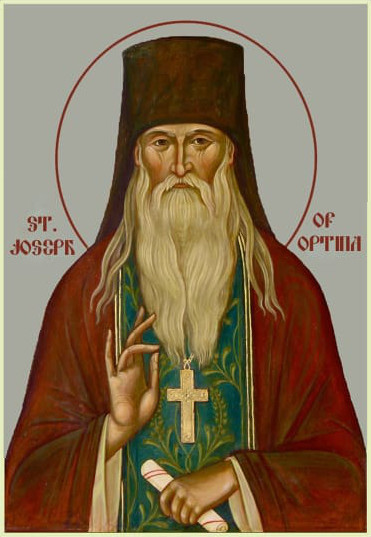
\includegraphics[width=\textwidth]{Images/StJosephOfOptina.jpg}
    
    \vspace*{\fill}

	\color{white}\LARGE \textbf{THE ELDER JOSEPH OF OPTINA}
\end{center}
\clearpage
\pagecolor{white}

\begin{adjustwidth}{.5cm}{.5cm}\itshape
	
	Editorial Note: 

    The following is an amateur reproduction of "The Elder Joseph of Optina", created out of a love for St. Joseph
    in the hope that others who would like to learn about his life can do so more easily than I was able to as this book has been 
    out of print for many years. When I finally found a copy I photographed each page and ran the photos
    through OCR software to extract the text, manually fixing the copious associated errors.

	While the text is as true to the original as possible, the page numbers do not match due to typesetting
	differences. I also left out many of the decorative images, 
	but included the original photos of people and places discussed. Original copyright info below.
	
	Please forgive any shortcomings, flaws, and mistakes. May God accept this small effort, 
	provide the correction and perfection it needs as he sees fit, and forgive my many offenses.\\
    \\
    St. Joseph, pray for us.\hspace*{\fill}-- Irenei\hspace*{1cm}
	
\end{adjustwidth}
\vspace*{\fill}
\begin{center}
	
	ISBN: 0-913206-53-0\\
	Library of Congress Catalog Card Number: 82-81456\\
	Holy Transfiguration Monastery, Brookline MA 02146\\
	Translation \textcopyright 1984 by the Holy Transfiguration Monastery\\
	All rights reserved\\
	Printed in the United States of America
\end{center}
\clearpage

\begin{center}
	\setlength\fboxrule{2pt}
	\color{red}\fbox{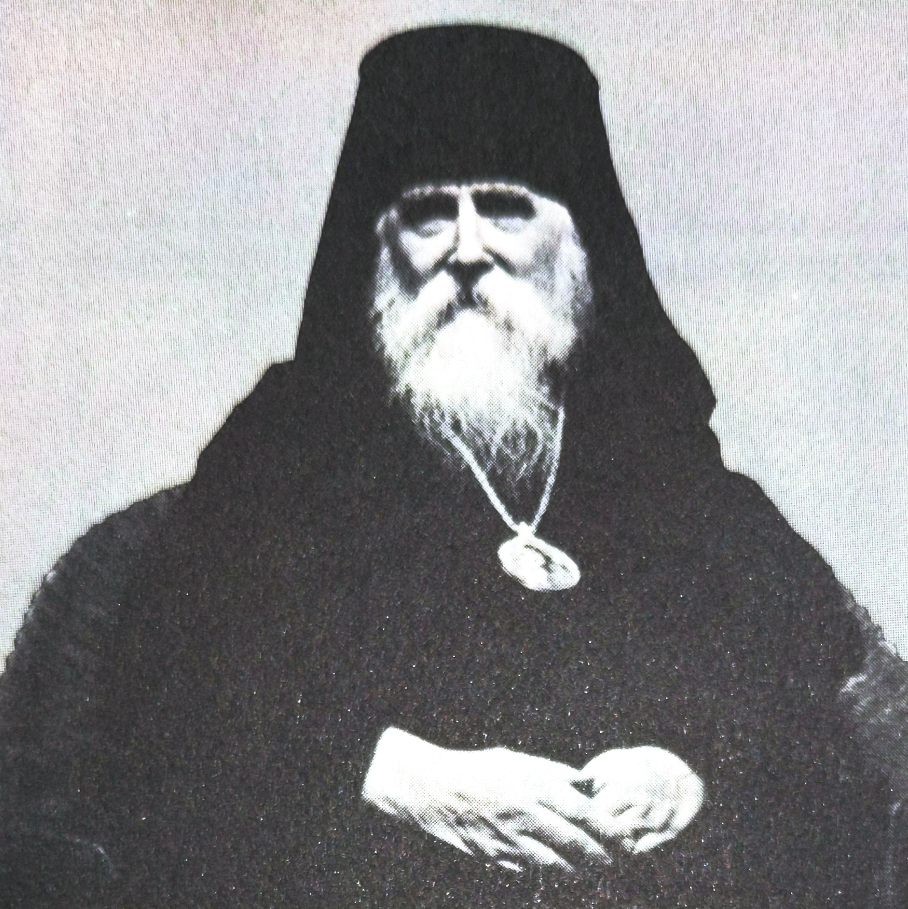
\includegraphics[width=2.5in]{./Images/Archbishop_Andrew.png}}\\
	\color{black}ARCHBISHOP ANDREW

	\vspace{1cm}
	\color{red}\fbox{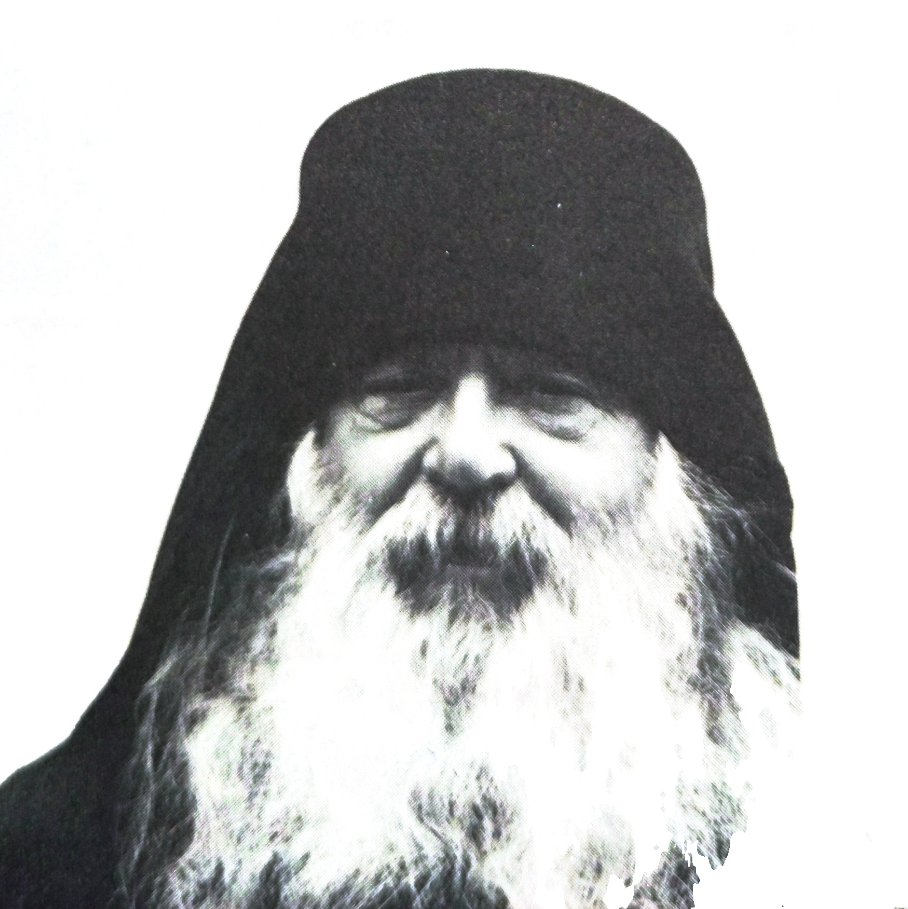
\includegraphics[width=2.5in]{./Images/Bishop_Nektary.png}}\\
	\color{black}BISHOP NEKTARY
\end{center}
\newpage
\vspace*{\fill}
\begin{center}
	\minicross
	\textbf{Dedicated to}
	
	\vspace{.5cm}
	\color{red}ARCHBISHOP ANDREW
	
	\color{black} of Spring Valley
	
	(1893-1978)
	
	\vspace{.5cm}
	and
	
	\vspace{.5cm}
	\color{red}BISHOP NEKTARY
	
	\color{black}of Seattle
	
	(1905-1983)
	
	\vspace{1cm}
	Devoted disciples
	
	of the last Optina Elders,
	
	faithful hierarchs
	
	of the Russian Church Abroad
	
	\minicross
\end{center}
\vspace*{\fill}
\newpage
\topskip0pt
\vspace*{\fill}
\minicross
\vspace{1cm}
\begin{adjustwidth}{1.25cm}{1.25cm}
``He was the closest disciple of the great Elder Hiero-schemamonk Amvrosy -- closest not in external things only, but in spirit, in strength of obedience, devotion, and love. He was in truth `the beloved child' of the Elder Amvrosy, who looked upon him with hope, who rejoiced in him seeing his spiritual progress, and whom he in every way preserved and guarded with his fatherly hand from all corrupting winds of conceit, vainglory, and pride.'' (P. \pageref{intro-excerpt})
\end{adjustwidth}
\vspace{1cm}
\minicross
\vspace*{\fill}
\newpage
\vspace*{\fill}
\begin{center}
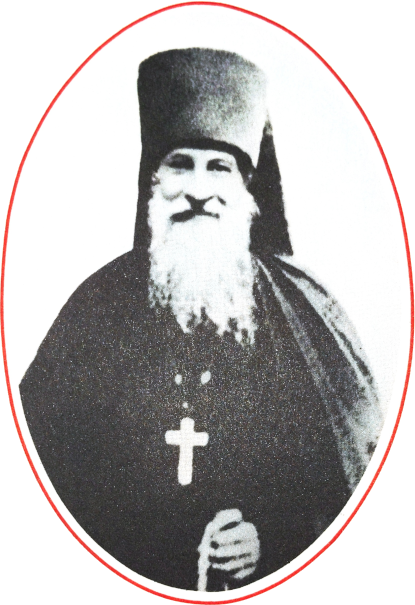
\includegraphics[height=17cm]{./Images/Elder_Joseph_Portrait.png}

\vspace*{\fill}
THE ELDER JOSEPH OF OPTINA\\
(1837-1911)
\end{center}
\vspace*{\fill}


\tableofcontents

%Chapters
\pagestyle{plain}
\addcontentsline{toc}{chapter}{FORWARD}
\chapter*{Forward\markboth{Forward}{}}

\begin{adjustwidth}{1.5cm}{1.5cm}
\centering
In the Name of the Father, and of the Son, and of the Holy Spirit. Amen.
\end{adjustwidth}
\vspace{.25cm}

\begin{adjustwidth}{4cm}{0cm}
	\color{red}
	\centering
	\textit{Upon whom shall I look, but upon him that is humble and quiet and trembleth at my words?}\\
	\hfill --Esaias 66:2
\end{adjustwidth}
\vspace{.25cm}
\hugered{F}OR MANY YEARS NOW, over a decade, we have had an English translation of the biography of the truly humble, meek, and quiet Elder of Optina, Hiero-schemamonk Joseph. The translation was made from the Russian by one of the senior fathers of our monastery, who had earlier translated Seraphim's Seraphim, the life of Pelagia Ivanovna. During these years, we have read the manuscript in the refectory during meals, and pilgrims and visitors to the monastery have read it in the guest quarters. Members of the community, pilgrims, visitors -- all have with one voice pleaded with us to print the biography. As in the instance of \textit{Seraphim's Seraphim}, once one begins to read this delightful and soul-profiting account, one is not able to put it down. So endearing is the image of the meek and joyful Elder that arises from the biography, that one is immediately drawn to him in one's heart.

Since a biography of the great Elder Amvrosy by John Dunlop has already appeared in English,\footnote{John B. Dunlop, \textit{Staretz Amurosy: Model for Dostoyevsky's Staretz Zossima} (Belmont, Mass.: Nordland Publishing Co., 1972).} with an extensive introduction concerning eldership and the founding and history of Optina, there is no reason that we should tire the pious reader with a repetition of names, dates, and details concerning Optina and her holy Elders. We certainly could never approach the work done by Dr. Dunlop, a work of love for which we are all indebted to him. Suffice it to say that the Elder Joseph was the spiritual son and disciple of the Elder Amvrosy and his successor as Elder of the Optina Hermitage.

The present publication, therefore, is a sequel to the book \textit{Staretz Amvrosy}, another chapter in the lives of the Optina Elders. It would be very edifying and spiritually profitable if others would undertake the translation and publication of the complete biographies of the other great Elders of Optina: Lev, Moses, Makary, and Anatoly. Then we would have in English a more complete series of these wondrous fathers. The biography of the Elder Joseph was the last of such biographies of the Optina Elders to be printed, since he reposed in 1911, only six years before that destructive Communist revolution which closed down Optina and its hermitage, as well as countless other monasteries, convents, and spiritual centers of the Russian land.

The biography of the Elder Joseph first appeared in Russian in 1911. It consisted of a brief account about the Elder Joseph written by a monk of the Optina Hermitage, and also of a much longer and more detailed account compiled soon after by the Shamordino Convent. The life compiled by the Shamordino Convent was reprinted by the Holy Trinity Monastery of Jordanville, New York, in 1962. In 1978, the Saint Herman of Alaska Brotherhood of Platina, California, issued a facsimile reprint of the 1911 edition, to which were added photographs from the collection of I. M. Kontsevich and an introduction by him.

In the present volume, we have placed first the two hundred page life by the Shamordino Convent, which covers the life span of the Elder from birth to repose; then we have appended the shorter account of some thirty pages written by an Optina monk whose name remains unknown to us. Although this anonymous account was the first to be printed, the author himself admits that he did not know the Elder Joseph for very long, and he narrates at greater length those incidents which he himself witnessed, giving detailed accounts especially of the last years, the repose, and the funeral of the holy Elder.

To these two lives we have appended the “Cell Rule of Five Hundred of the Optina Monastery,” since it is mentioned in the life and was nowhere to be found in English. We have also translated and added a letter by the Elder Joseph entitled, “May Orthodox Christians Pray For Non-Orthodox Christians, And If So, How May They Pray For Them?” since this is a very timely subject and of interest to many of the faithful, both native and converts, living in the midst of non-Orthodox. This is the only printed letter of the Elder which we have been able to find. It first appeared in the religious periodical \textit{Edifying Readings}, Moscow, No. 3, 1901, under the name of Hieromonk Joseph. For some time we were not able to ascertain if the letter was by the Elder Joseph of Optina or some other Hieromonk Joseph. However, upon locating the above-mentioned periodical in the St. Vladimir's Theological Seminary library, we verified that the letter indeed was by "the Superior of the Optina Skete, Father Joseph.” In the Life it is mentioned that at the time of the holy Elder's repose, there was every intention to print all his collected letters, but-alas-because of the great upheaval of the revolution, this never came to pass. Therefore, this one letter of the Elder, aside from its timely content, becomes even more precious, since until others are found, it must serve as representative of his other correspondence.

The lives and teachings of holy men and women are a great source of instruction to the faithful for they serve as a living example-something concrete, not abstract. In that they fulfilled the injunctions and commandments of the Lord, the saints are the incarnation of the beatitudes, the “living Bible,” “the perfection of the Gospel” as we chant in the hymns of the Church. Though being “subject to like passions as we are,''\footnote{James 5:17.} “out of weakness they were made strong''\footnote{Heb. 11:34.} because of their love for God and their struggles for righteousness' sake, and are therefore especially able to help us and instruct us. Their example and teaching, like that of Holy Scripture, are relevant for every generation and are always contemporary. So is it with the Elder Joseph. This present volume, like that of \textit{Papa-Nicholas Planas}\footnote{\textit{Papa-Nicholas Planas} (Boston, Mass.: Holy Transfiguration Monastery, 1981).} and \textit{Staretz Amvrosy}, are genuine treasure troves, inexhaustible mines filled with a wealth of Orthodox piety and teaching rarely to be met with elsewhere. Take for example chapter five entitled, “The Elder Joseph's Instructions.” It is filled with spiritual knowledge which comes from experience, knowledge which can be applied by all of us, each in his own context. How timely is the observation of the Elder concerning dreams and apparitions given on the occasion when a young woman had reposed and began appearing to a friend. He writes, “The blessed Diadochus advises us not to trust even true, grace-filled apparitions. The Lord will not rebuke one for not trusting, since he does so not out of disdain for God, but in order not to fall into demonic deception” (p. 178). This is but one of many such instructive and soul-benefiting passages one encounters in this small book.

The Monastery of Optina, with its skete and dependencies, was officially closed by the God-hating Communists in 1923. The Elder in his foreknowledge appears to have foreseen this, for on one occasion he warned, “... or else, because of our disobedience, the Lord will take away the Elders and He will leave no one” (p. \pageref{ch5obedience}). The main church of the monastery proper, dedicated to St. Mary of Egypt, was dynamited --its ruins can be seen to this day (see p. \pageref{saint-mary}). The fate of the other churches and chapels was similar. They were plundered and finally dismantled. Some of the buildings were put to other uses. The small cottages (cells) of the skete, where the Elders and fathers lived out their lives, were given to workers as residences and have thus survived to this day. We have heard from unofficial reports that native visitors (foreign visitors are prohibited from visiting the area) have been shown the cell of the Elders Amvrosy and Joseph by its present occupants as well as other places of interest connected with the Elders and monastics who lived there when it was still a monastery and skete. (It is to be understood that some of these visitors are believers who come as pilgrims to pray, and others are native tourists who come out of curiosity. Of late in the Soviet Union there has been a revival of interest in the cultural and national monuments of the past.) This has annoyed the local authorities and they have threatened the present occupants of the cottages with eviction if they continue this illegal work of serving as guides to visitors.

We have also heard from a visiting American professor, who stayed in the Soviet Union for some time, that he was shown a building in Moscow where, according to a Soviet professor, the archives and personal papers of the Optina Monastery and Hermitage have been stored for many years, having been transferred there at the time of the destruction of the monastery. If this is true, then there is hope, if the world does not end shortly, that in the future many documents and personal papers of the Optina fathers may see the light of day, possibly even the correspondence of the Elder Joseph, if it has been preserved. Let us hope and pray that God grant it.

Some years ago, we had the thought to dedicate this small book to Fr. Vladimir of the Holy Trinity Monastery in Jordanville. Fr. Vladimir has a special love for the Elder Joseph and has been encouraging us throughout the years to print the book. However, knowing his modesty, we are certain that if it were dedicated to Fr. Vladimir, it would be a cause of embarrassment to him. Therefore, we have decided that it would be appropriate to dedicate it to two of our hierarchs of blessed memory, Archbishop Andrew of Spring Valley and Bishop Nektary of Seattle, direct disciples of the last Elder of Optina, Nektary, who died in exile in 1928. We know that this will be pleasing to Fr. Vladimir also, since Vladyka Andrew was our common spiritual father for some years. We knew Vladyka Andrew well and on almost every occasion that we went to him --and they were countless-- he would inevitably tell us some story concerning Optina and his experiences there, especially concerning his beloved Elder Nektary, whom he continued to visit secretly, even after the Elder's exile. The Elder Nektary actually reposed in his arms, literally under the epitrachelion of Vladyka Andrew, who was then the young priest Fr. Adrian. Vladyka used to tell us that of all the clergy of the deanery to which he belonged he was the only one to survive the atheist persecutions. All the other clergy were either shot immediately or perished in the camps.

Bishop Nektary would also continuously reminisce concerning Optina and its Elders. On his one visit to our monastery, after our meal in the refectory he related to us concerning the last Elders Theodosy ( + 1920), Anatoly the Younger ( + 1922), and Nektary ( + 1928). Vladyka said that the Elder Theodosy was the embodiment of wisdom and theology, Anatoly of love, and Nektary of humility. He would also speak concerning his memories of Optina and its Elders to our abbot and one of our senior fathers who visited Seattle yearly. Vladyka's blessed mother, who in the tonsure later took the name Nektaria nun, used to take him to Optina from the time that he was a child. She was actually at Optina when the Soviets began closing the monastery, and was arrested with all the clergy, monastics, and visitors who were there. But seeing that she was a simple, pious pilgrim, the authorities released her after one day of custody. Notwithstanding, she continued to take her son Oleg (that was the name of Vladyka Nektary in the world) to see the Elder Nektary at the place of his exile right up to the end, even though this was quite dangerous. It is only appropriate then that this present volume should be dedicated to the blessed memory of these two hierarchs. We wish to thank Mrs. Irina Hay of Lexington, Massachusetts, for her inestimable help in rendering certain passages from Russian into English and her numerous suggestions concerning the whole manuscript. We wish to make acknowledgment also of the service rendered by Mr. John Bruk of Roslindale, Massachusetts, in reading the manuscript and offering his suggestions. We are also indebted to Mr. Anthony Pasquale of Providence, Rhode Island, for providing us with the photograph of the Elder Joseph on page \pageref{elder-joseph-bed}.

Remember us, dear readers, in your prayers unto the Lord.

{
	\vspace{.5cm}
	\hspace*{\fill} {\color{red}HOLY TRANSFIGURATION MONASTERY}
	\vspace{.5cm}
}\\
\textit{Feast of the Holy Apostles}\\
1984
\addcontentsline{toc}{chapter}{The Kozelsk Monastery of the Entry of the Mother of God into the Temple}
\chapter*{The Kozelsk Monastery of the Entry of the Mother of God into the Temple\\ (Kozelskaya-Vvedenskaya)\footnote{A. A. Pavlovskiy, comp., \textit{A Comprehensive Illustrated Guide to the Monasteries and Holy Places of the Russian Empire and Athos} (Nizhny Novgorod, 1907), pp. 246-8.}\markboth{The Kozelsk Monastery}{}}

\hugered{T}HE KOZELSK Optina Hermitage of the Entry of the Mother of God into the Temple is located 4 versts (2 \sfrac{2}{3} miles) from the city of Kozelsk which lies on the Ryazan-Ural rail line. It is situated on the picturesque right bank of the Zhizdra River. According to tradition, this hermitage was founded prior to the fifteenth century by a certain repentant ataman (head) of a den of thieves, Opta, who likewise founded the Optin-Troitsky Monastery in the Orlov province.

In the fifteenth century monks and nuns lived adjacently in the monastery, but in 1499 the latter were taken to the city where they founded their own Convent of the Ascension. In the beginning the hermitage did not have great means, and in 1724 it was closed and turned into a parish, while the monks were transferred to Belev, to the Monastery of the Transfiguration of the Saviour.

At the intercession of local citizens, the Shepelevs and Ardatov, within two years after its closure the monastery was again restored at the expense of those who had interceded. In 1764 the hermitage became self-supporting, but apparently it again began to fall into decline, until it was restored by Archimandrite Makary in 1795. From then on, better times began for the hermitage, and it began to acquire great renown.

Among the number of holy things to be found in the Kazan winter church is a wonderworking icon of the Mother of God of Kazan, donated in 1808 by the landowner Soburovaya. In addition, there is a specially venerated icon of the Beheading of Saint John the Forerunner, in whose honor there is at the hermitage the Skete of Saint John the Forerunner. The Great Prince Constantine Constantinovich has here also donated a perpetually-burning icon lamp. The monastery's vestry is not large. The church feast is on the day of the Entry of the Mother of God.

The monastery has land in various provinces amounting to two thousand \textit{dessiatinas} (5,400 acres) of forest and agricultural land. There are about three hundred brethren under the direction of Archimandrite Xenophont.

\clearpage
\subtitle{
	Optina Hermitage\footnote{\textit{The Complete Orthodox Theological Encyclopedic Dictionary}, s.v. ``Kozelskaya-Vvedenskaya Optina.'' No author, editor, or date given (approximately 1910).}
}

Men's hermitage (self-supporting from 1764) in Kaluga Province, 4 versts from the city of Kozelsk on the river Zhizdra. The exact time of its founding is not known. The hermitage was destroyed by the Lithuanians and left desolate. It now has 6 stone churches, a hospice, guest-house, house, hospital. Eldership -- preserved in few monasteries -- is observed in the hermitage. Governed by an abbot. Approximately 310 brethren.


% START PART I
\titleformat
	{\part} % command
	[display] % shape
	{\bfseries\Large} % format
	{
		\begin{center}
		\thepart
		\end{center}
	}
	{0.5cm}
	{
		\vspace{-1.5cm}
		\begin{center}
			\color{red}
	} % before-code
	[
			\color{black}
			\vspace{1cm}
			\bfseries\normalsize		
			A publication of the\\Kazan Ambrosiev Women's Hermitage\\
			\vspace{2cm}
			{
\includegraphics[height=5cm]{./Images/Part_Emblem.png}}
		\end{center}
	]
	
\part{A Sketch of St. Joseph's Life\\\hspace*{2em}\small{from the} \emph{\small{Kazan Ambrosiev Women's Hermitage}}}

% Shift Part 1 chapters over 1 CM in table of contents
\addtocontents{toc}{\protect\begin{adjustwidth}{1cm}{0cm}}
\addcontentsline{toc}{chapter}{Preface}
\chapter*{Preface}
\hugered{I}N PUBLISHING the present sketch of the life of the ever-memorable Elder of Optina Hermitage, Hieroschemamonk Joseph, the Saint Ambrose Women's Hermitage of Kazan\trans{This was the formal title of Shamordino Convent.} has had as its aim, on the one hand, to express thereby its deep appreciation and love toward their reposed spiritual guide, and on the other, to give at first at least a small consolation to all the spiritual children of the Elder Joseph and to all who revered him, inasmuch as it is well known that after the passing away of someone beloved, recollections of him serve as a great source of comfort.

Having quickly collected everything that is known about this wondrous Elder, the Ambrosiev Hermitage rests assured that Optina Hermitage will undertake the editing of all the material at hand, and will concern itself with the publication of a complete and detailed biography of this Elder, great in his humility, even as Optina has heretofore with such love labored in publishing the excellent descriptions of the lives and ascetic struggles of its earlier great Elders.

\hfill November 1911

\addcontentsline{toc}{chapter}{Introduction}
\chapter*{Introduction}

\hugered{O}N MAY 9, 1911, the Optina Elder, Hiero-schemamonk Joseph, fell asleep in the Lord. \label{intro-excerpt} He was the closest disciple of the great Elder, Hiero-schemamonk Amvrosy--closest not in external things only, but in spirit, in strength of obedience, devotion, and love. He was in truth “the beloved child” of the Elder Amvrosy, who looked upon him with hope, who rejoiced in him seeing his spiritual progress, and whom he in every way preserved and guarded with his fatherly hand from all corrupting winds of conceit, vainglory, and pride.

This child of obedience was reared within the walls of Elder Amvrosy's humble, lowly hut, which was permeated with the precepts of the great Elders Lev and Makary and with the prayers of their successor, the Elder Amvrosy. Here in this small cell, which became for him “the school of piety,” he undertook the study of what is in truth the highest of sciences, monasticism, and in time he also became a director of monastics. And how simple and unassuming all this was; by many it was not even noticed.

The character of Fr. Joseph was distinguished by exceptional modesty, sensitivity, and compliance; and with time, these qualities deeply penetrated his whole being and developed into the great virtues of humility, love, and angelic meekness.

Of those who knew Batiushka Joseph as a simple monk and cell-attendant of Elder Amvrosy, who does not remember his manner when he went at times to the women's side of the hut: his humble step, lowered eyes, short answer with a bow, his invariable modest smile of greeting, always inconspicuous, never obtrusive. Nonetheless, even then everyone almost instinctively turned to him with special reverence, for they perceived something in him which placed him above all others.

At that time, the Elder, Fr. Amvrosy, had a senior cell-attendant, Fr. Michael, who on entering the women's section of the hut, liked to speak a little and to say something instructive. Then the hut would become enlivened-they would ask various questions, and at times even soft, restrained laughter would be heard. However, when Fr. Joseph went, everything would become quiet, everyone would become serious, and many would trustingly communicate to him their griefs or a message for the Elder.
\chapter{Life In The World}
\hugered{E}LDER HIERO-SCHEMAMONK JOSEPH, in the world Ivan Evfimovich Litovkin, was born on November 2, 1837, in the village of Gorodishcha, in the Starobelsk District of the Kharkov Province. His parents Evfimy Emilyanovich and Marya Vasilyevna Litovkin were simple people, but very pious, kind, and intelligent. His father was the village-head for seventeen years and enjoyed great respect and love. Both he and his wife were very merciful to the poor; they gave from their possessions with a generous hand, and often without the other's knowledge. Evfimy Emilyanovich lended to whomever was in need of money, although it would sometimes happen that he did not get it back. He loved to receive into his home monks whose obedience it was to ask for alms, and without fail he would give to each of them five gold rubles for his monastery.

In accord with the ways of olden times, they loved very much to go to church and to read spiritual books, especially the lives of the saints. They had six children, three sons and three daughters. When the second son was born, his parents named him John in honor of Saint John the Almsgiver,\trans{In combination with the name of his patron saint, the writer uses the more formal Slavonic “Ioann” (John). “Ivan” is the popular form of the name.} for whom they had a special devotion. Truly loving their children, they tried to give them Heavenly treasure rather than earthly wealth; therefore they raised them in the fear of God, piety, and obedience. The father had a very lenient character, but the mother was more strict. The children feared her very much, but loved her just as she loved them. Of all the children, the father loved Ivan most, who even in his facial features resembled him. Once he took him for a ride on the droshky and punished him along the way for some prank. Afterward the gentle father felt remorse for a long time and would say, “Oh, he's just a boy, and I struck him!”

Ivan's older sister Alexandra, who especially loved him, began to teach him grammar, so by the time they put him in school, he was already able to read. In general, he was a good student. “In school,” Batiushka related, “they didn't punish me; but once the teacher ordered me to punish my younger brother Peter. This was very hard for me and pained my soul.”

The mother would take all the children with her to church, and at home would make them pray together with her. According to stories told by the Elder himself, from his early childhood he loved to be in church, where he even sang in the choir. “I remember how mother would wake me to go to Matins and the Liturgy. I didn't want to get up out of bed early, but there was nothing to be done: I had to get up. Because of that, in church and for the whole day afterward I used to feel so good and happy in spirit!”.

Then he would continue, “At home, mother would also make me read the Akathist to the Saviour or to the Mother of God. Sometimes it happened that we would be standing at prayer and suddenly through the window we would see a bear being led along the street; there would be a lot of noise and many people. It was so frightening! We would begin to pray even more zealously.”

The visitors hearing this would sometimes ask him, “Surely the children wanted to go closer to the window and have a look at these strange sights?”

“No, that was impossible; our mother was strict," he would say.

From childhood Ivan was sickly; because he was scrofulous, he became hard of hearing in one ear and near-sighted. In addition, he often met with various mishaps. When he was still small, his sister accidently set him on a very hot stove-couch. Another time, he scalded himself with water. At another time, a boy who was racing by knocked Ivan off his feet, and he bit off the tip of his tongue. Notwithstanding, he was a very lively and happy child by nature.

His sister, who afterward became a nun, related that little Vanya\trans{The affectionate and diminutive form of "Ivan.”} was a very affectionate child. With his tender and sensitive soul, he could somehow feel another's grief, although his inborn modesty and shyness did not allow him to speak out. When he noticed that someone at home was melancholy, he would quietly linger about him and then snuggle up and caress him fondly.

The father always said of him, “Something special will come of this boy.” It is worthy of note that if Evfimy Emilyanovich said something of his children, it later came to pass exactly so. Among other things, he expressed even then the desire that one of his children become a monastic. The first to respond was his daughter Alexandra (afterward the nun Leonida), and after her, in time, his son Ivan. Vanya's catechist, a protopresbyter of very good life, on his part said of the boy, “Wait and see, something unusual will come of him.” Thus from earliest childhood, all noticed in him the special seal of the favor of God.

When Vanya was four, he lost his good father, who died suddenly. Nevertheless, the little one fared well under the wings of his tenderly loving mother. When Vanya was eight years old and was playing with friends, his face suddenly changed; he raised his head and hands upward and fell unconscious on the spot. They carried him home and put him to bed; when he revived, they began asking him what had happened. The boy said that he had seen the Queen in the air.

“Now why do you think you saw the Queen?” they asked.

“Because she had a crown with a cross,” he answered.

“Well, why did you fall down?” they asked again.

In reply to this, he cast down his little eyes and quietly said, “Near her there was such a sun ... I don't know, I don't know how to say it!” he added quickly and began crying.

This wondrous vision left a deep impression on the soul of the eight-year-old child. From that time on, he completely changed; he became quiet and thoughtful, began to withdraw from children's play, and was constantly with his mother. The gaze of his gentle eyes became still deeper, and his child's heart became inflamed with faith and love for the Heavenly Queen.

Soon after this, and not long after they had moved into a newly built house, there was a great fire in their village. The child saw the fear of those at home and he too understood the danger. Not knowing where to turn for help, he stretched out his little hands toward the church near their home, named after the Protection of the Most Holy Mother of God, and cried, “Heavenly Queen! Leave us our home! After all, it's completely new!” The child's prayer was heard; everything around burned, but the home of the Litovkins remained unharmed.

By this time, Ivan's older brother Simeon was married, as was also his sister Anna. Before two years had passed, the mother took her daughter Alexandra to the Borisovsk Hermitage and left her there, having entrusted her to the Heavenly Queen. All at home were much saddened by the departure of the gentle and loving girl, but Vanya grieved most of all, and he wept over the separation from his beloved sister.

But soon a new, still more difficult separation awaited him. A year later, in 1848, when he was eleven years old, cholera appeared at their village; and the first victim to this terrible visitor was his mother. The boys Ivan and Peter now became orphans. At the funeral, little Ivan exclaimed with much grief, “Heavenly Queen, what are you doing? Sister went away to the convent, and now you've taken Mama away from us!” Everyone present involuntarily began to weep when they heard the outpouring of the child's grief; the priest, that same protopresbyter who had foreseen in the boy the future chosen one of God, wrote down these words and recorded the time. Later they found out that his sister Alexandra Evfimovna, who was living in the convent, had known nothing of the death of her mother; on that very day and hour she became very despondent, and falling into a light sleep she saw a coffin with her mother inside floating down a river and heard the very same words, "Heavenly Queen, what are you doing? ..." and the rest.

From that time on, the life of the orphans changed markedly. The older brother, Simeon Evfimovich, became the head of the household, and although he was a very capable person, he was subject to a great weakness--he drank wine.\footnote{The Elder always spoke well of him, as of an honorable and noble person, whom evil company had led to a dissolute life because of this weakness in his character. While in the military service he was deprived of his rank several times because of this weakness, but afterward he re-qualified. The Elder saved two of his letters which he even planned to have printed as an example of humble confession and sincere, deep repentance.} After the mother had reposed, he very soon left home, and all of the parents' estate deteriorated; after a year, when Alexandra Evfimovna came from the convent, she found nothing at home. Her relatives begged her to stay and take care of the orphans; Ivan especially wept inconsolably and begged his sister not to leave him. She related, “They would grab me by the belt with their little hands and weep bitterly, 'Sister, take us with you to the convent. There's no one for us to live with here!' My heart simply bled, looking at them. Vanya would even repeat these words in his sleep."

It was unbearably difficult for Alexandra Evfimovna to part from them, especially from her favorite; but she firmly decided to give up everything and go her own way for the sake of God, and to take care of her small brothers from the convent when possible. As a result of this grief and anxiety which was beyond her strength, she suffered ill health for the rest of her life. Although she was later healed by the Kozelshchansk icon of the Mother of God of an agonizing illness which befell her soon after returning to the convent, she always remained weak and sickly with overwrought nerves. She related afterward that she had almost decided to take Ivan with her and to place him in the monastery closest to Borisovka, but the above-mentioned protopresbyter convinced her not to do so. Apparently, it was pleasing to the Lord that His faithful servant be tested.

The older brother kept Ivan with him, while the married sister took the younger Peter. But soon Simeon Evfimovich was constrained to go and live with strangers, and therefore he sent his brother elsewhere. From that time on, the trying experiences of a bitter orphanhood began for him. The poor child who had been used to the tender kindness of his parents was forced to see and endure much. His lot was difficult and harsh; he was tried in everything: cold, hunger, beatings, and labor beyond his strength.

At first his brother placed him with a tavern keeper whom he knew. Here the poor boy was especially miserable. His brother came often to play cards and drink wine with the owner, and the boy was forced to do everything by himself since he and the tavern keeper were the only two living there. Unable to endure such a life, Ivan left his master and returned to his brother. Although his brother felt sorry for him, he soon placed him with an Armenian in Nakhichevan. He did not stay there long, however, and was placed in a grocery store in Taganrog. Here he had to go for food to the owner's apartment at the end of town. Once while he was going to the store with lunch pails, he became very tired, sat down to rest, and right on the spot fell into a deep sleep. While he slept, someone took off his boots and stole the lunch pails, and for that reason the police took him to the station. At home, of course, he received punishment from the master for both the boots and the dinner.

Ivan left this master also and went by foot to Novocherkassk, to his cousin who was a deacon there. He arrived there famished since he had had no more than a few biscuits with him. Concerning this trip he said, “For two days I ate absolutely nothing. I just didn't know how to beg, and people wouldn't give of themselves; so I humbled myself by not eating. When I came to Novocherkassk, I searched for the church where my cousin served. While waiting for the Liturgy to end, I sat on the church porch. Here two Cossack women with some rolls passed by me, and one of them said, 'This boy is probably an orphan and hasn't eaten anything,' and she gave me a roll. How happy she made me; it seemed so delicious to me, just like manna from Heaven!”

Although it was pleasant living with his cousin the deacon, it was impossible to stay for long. The latter sent him to his father-in-law, a priest. Here everyone came to love Ivan very much, and he lived well there. Fr. Joseph used to recall one episode from his life with this priest. Once at Christmas-tide, the priest's daughter proposed to tell fortunes in the mirror at midnight; she was frightened to sit alone and so she sat him down beside her. “I really wanted to go to sleep,” he said, “and in order not to fall asleep, I began to pray; so we saw nothing.”

Later, his sister Alexandra succeeded in placing her brother in an iron shop, but it was equally difficult for him everywhere. Once the master, a former church warden of the cathedral, sent him to give a message to the workers who were at the top of a structure. He climbed up quickly, but when he started to descend, his head started to spin and he fell down unconscious.

When he was completely without a job, he would apply for day labor. “He who wants to labor,” he said later, “always finds something.”

He would have to carry five sacks of flour weighing thirty-six pounds each and other such loads. Once while hauling boards from rafts, he stumbled, fell into the water, and began to drown, since he had fallen between two rafts and there was nowhere he could swim out. Suddenly, some invisible hand pulled him up to the surface of the water; the Lord had saved him from death.

On another occasion, he was taking leather goods somewhere with the proprietor. They stopped to spend the night at an inn. The owner went to sleep in the cottage, while Ivan stayed out in the cart. During the night there was a fire, and in the confusion everyone forgot about him. From fatigue he slept so soundly that he heard nothing, and when he awoke in the morning, he could not tell where he was, since everything around him had burned down.

Still another time, Ivan had to go from Stavropol to Rostov to find a position with some master. It happened that a certain Armenian had bought potatoes in Stavropol and was also heading for Rostov with two carts. Ivan made arrangements with him to be taken there, although both of them had to go by foot a good part of the way since the carts were loaded with potatoes. They came to the Don where there was a ferry and barracks built for the Cossacks. But the Don had begun to overflow, because a wind blowing from the sea made the water rise. The Cossacks refused to take them across. Not wishing to lose time, the Armenian proposed to Ivan that he travel with him along the shore. They went, but the water kept rising more and more. Then Ivan, not heeding the pleas of the Armenian, returned by foot to the barracks. He had to walk there in water up to his belt. On reaching the barracks, he spent the night there. The soldiers gave him dry shoes; but when he began taking his boots off, it turned out that they had frozen to his feet. By the next day the water had gone down, and they took him over to the other side of the Don, where he continued on his way to Rostov by foot.

Thus young Ivan constantly experienced dangers, but the Lord preserved the orphan everywhere. Despite the fact that his youth was spent in coarse and often corrupt surroundings, no evil injured his pure soul. He never drank wine or played cards. Once, he was served some weak grape wine called \textit{chikhir} when he was in great grief, but having drunk a small glass, he immediately felt tipsy, and his head began to spin. Thereafter he vowed to himself never again to take into his mouth any kind of wine. “If a person becomes tipsy from such weak wine, drunk in such a small amount, then what would happen to him if he should drink much?” thought the judicious youth,

He was completely indifferent to the female sex. He was once asked, “Did you like someone in the world?” Whereupon he answered with a naive simplicity which best of all proved his honesty and innocence, “Well, since I was nearsighted, I couldn't make out anyone from afar, and I was ashamed to approach anyone closely--I was shy. It used to be very difficult for me when the master sent me to call someone when we had guests. There was no way I could make out whom I was supposed to approach."

In the world, he generally experienced melancholy, and the unfailing companion of his sorrowful life was prayer--the only inheritance left him by his pious parents. His only place of comfort was the church to which his piety always drew him.

Finally he succeeded in finding a good position in Taganrog with the merchant Rafailov, who being a pious person, went with him to the church services. His job was to take the rye which the \textit{chumaks}\trans{Ukrainian ox-cart drivers.} brought in from various places, and then to distribute it in the city to various shops, both Russian and Greek. During the summer there was a lot of work, in the autumn less, and in the winter there was absolutely nothing to do. So after the coming of autumn, the master suggested to Ivan that he go to the village mill which was leased to a certain Ukrainian man. Not liking the noise of many people, Ivan was glad to live in the quiet of the village. During that winter, there was almost nothing for Ivan to do, since the mill was being repaired by the man who was leasing it.

The old miller turned out to be a pious man; he always went to the church services on feast days. Both of them became close friends with the parish deacon, and together they would read the holy books which were found there at the church. On feast days, the three of them would have heartfelt conversations. Ivan Evfimovich lived this way until spring. He still had no thought of monasticism, but about this time he received a letter from his sister, the nun Leonida, in which she suggested that he take up the monastic life in the skete of Optina Hermitage, long renowned for its spiritually experienced Elders. Then there began to burn in Ivan Evfimovich a strong desire to leave the world and to enter a monastery.

The master had come to love this well-behaved youth on account of his modesty, honesty, and love for work, and he had become so well-disposed toward him that he had begun to consider giving him his daughter in marriage. Once after Liturgy, the eldest son of this merchant said to his parents, “Today in church I didn't pray so much as I watched Ivan Evfimovich and was moved by him; how well he stands in church, how diligently he prays, looking not once to the side, but entirely rapt in God. We couldn't find a better man for our sister; we shouldn't let him get away.” Thus, the good qualities of his soul were manifest and attracted love and respect.

But the young Ivan was far removed in thought and heart from worldly attachments. His pure soul was now attracted to live with the hermit monks. His favorite pastime from childhood had been reading the lives of the saints. Now these wonderful examples, illumined by the splendor of Heavenly glory, rose before him and outshone all the beauties of this world. His soul did not find full liberty for itself in the workaday, bustling world, and within him there appeared an unquenchable desire to tear himself from the commotion of life, at least for a while, and to go on a pilgrimage to worship the holy places. His cherished dream was to go to Kiev and with trembling heart and lips to venerate the holy relics of the living temples of the grace of God which accomplishes all things. This dream moved him to pray fervently, “Cause me to know, O Lord, the way wherein I should walk."\footnote{Psalm 142:10.}

When he learned of Ivan Evfimovich's desire to go on a pilgrimage to Kiev, Rafailov zealously set about to persuade him to remain in Taganrog, and revealed his desire to give him his daughter in marriage.

“It's always like that,” said the Elder years later, as he recalled this circumstance. “As soon as a person starts thinking of going on the path of salvation, right away there appears an obstacle and temptation.” Truly, when he lived among sorrows, adversities, and trials, people passed him by without noticing him; but as soon as his soul began to separate itself from earthly concerns, the world was now at his bidding. For the poor orphan, his entire future stretched before him as one of endless need and constant dependence; then of a sudden, an offer of marriage to a rich merchant's daughter and the possibility of becoming an independent and wealthy person. Surely, is this not a temptation? Is it not a snare for the inexperienced fledgling? But he who was already ensnared by the love of Christ quickly and easily escaped by immediately coming to a decision, whereas another would likely have wavered. Not hesitating for a moment, he again asked his master's permission to go on a pilgrimage, and the rest he entrusted to God's will and direction.

His good master Rafailov, on seeing the sincere and fervent yearning that the youth had for God, dared not hold him back any longer. He dismissed him with peace and love, and only requested that by all means he return and stay forever in Taganrog.

With a knapsack on his shoulders, the young traveller set off for the goal of his cherished thoughts. Sacred Kiev was already standing before his mind. Along the way he stopped at his deserted birthplace, and after venerating his parents' graves, he cast a farewell glance at the place where his happy childhood had flashed by so quickly, and he continued on. Stopping by the Holy Mountains of the Kharkov Province, he spent several joyful days there and came to compunction in his soul, observing the peaceful life of the monks of that quiet monastery.\trans{This refers to the Monastery of the Dormition located in the Holy Mountains.} Nevertheless, he did not want to remain there; he was attracted to where the broad Dnieper casts its quiet waves.

From the Holy Mountains he set out for the last stop on his journey, the Borisovsk Women's Hermitage, where as was mentioned before, his sister the nun Leonida lived.

Mother Leonida was a frail, tender soul, loving and gentle. Left without any means, she was constrained to live as a cell-attendant, and besides her monastic obediences, to fulfill all the heavy chores for the nuns with whom she lived. But having lost her health, she couldn't work at all, and another nun took her into her care and subsequently became her spiritual friend. At that time the Borisovsk Hermitage was noted for its strict monastic life and for its being under the spiritual guidance of the Elders of Optina. In the Hermitage also, there were experienced and wise Eldresses guiding the young sisters. Mother Leonida and her friend the nun Anatolia were under the immediate supervision of the wise Eldress Schema-nun Alypia, who in turn was a disciple of the Optina Elders Leonid and Makary. Once when she was at the Optina Hermitage with her Eldress, Mother Leonida with tears told the Elder Makary of her grief over her orphan brothers and expressed her fervent desire that her beloved Vanya go to a monastery. “Don't worry," the Elder said to her affectionately, “he'll be a monk.”

At the time when Ivan Evfimovich came to Borisovsk Hermitage, the Superior was the Abbess Makaria, who led an exalted spiritual life. Discipline under her was very strict; for example, nuns were not allowed to receive men in their cells, even though they be their own fathers. Only men doing necessary work for the cells were allowed in the court or in the entrance hall. The sisters would prepare food for them and carry it out to the porch; in the wintertime, the workers carried the small pots to the reception room and ate there.

Learning about these strict rules of the convent, and that there would be no other chance of seeing the one person who was close and dear to him, the loving brother did not falter at the obstacle which had arisen. He took a shovel and axe in hand and went to the indicated cell in the capacity of a worker in order to chop firewood and clear the snow. Mother Leonida, half dead from sickness, shed bitter tears as she gazed through the window at her "little brother,” and she couldn't get enough of looking at him. With what love, with what tenderness would she have embraced her little orphan, but the vow of obedience is holy, and she submitted and prayed. The wise Eldress Alypia, knowing the spiritual condition of her disciple and the pain and distress of her tender and loving heart which had already suffered so much agony, decided to allow the modest and God-fearing boy into the cell, and took upon herself full responsibility before the strict abbess.

O happy hours! How many tears of joy and sorrow were poured forth here, how many memories were brought before them, how much was said that was heartfelt, intimate, profound! The Eldress Alypia more than once listened to their conversation, and noticing in the youth a true yearning for God and readiness for struggles, said to him, “Forget your Kiev and go to Optina, to the Elders.” Ivan glanced questioningly at his sister and in her eyes read the answer, “Obey.” It was enough; Kiev was forgotten.

The next day, with the same knapsack on his shoulders and with a last blessing from the Eldress and his sister, who had taken the place of his mother, Ivan set out on his way anew, but now not to where his heart had attracted him, but whither the hand of obedience had directed him. Reaching Belev, he stopped at the convent to get directions for Optina Hermitage. The nuns of this convent, like those of Borisovsk, were under the Elders. The Elder Makary was no longer living, but in Optina a new lamp had been kindled, the immediate disciple of the Elders Lev and Makary, the Elder Amvrosy.

It happened that on this day two Belev nuns were driving to Optina; upon learning that the young traveller had come from afar seeking the Elder, they took him along on the driver's seat. Having arrived at Optina, the nuns went to the Elder Amvrosy, and in the course of the conversation they said to him, “Batiushka, we have also brought Brother Ivan along with us.” They called him “brother” in jest, because of his monastic inclinations.

The Elder looked at them seriously and said, “This Brother Ivan will prove useful to us and to you.” Thus the great Elder Amvrosy, not yet knowing of whom they spoke nor yet having seen him, already foresaw his high calling and he prophetically foretold what benefit Ivan would subsequently bring to Optina itself and to all the women's convents under the Elders.

The new arrival stood trembling before the Elder Amvrosy; simply and unpretentiously, Ivan told him of his life and asked for a blessing to go to Kiev, whither his soul had been long yearning, and where, perhaps, he could stay permanently. The clairvoyant Elder struck him lightly on the head and said, “Why do you want to go to Kiev? Remain here.” Again longed-for Kiev eluded him, but Ivan believed deeply that the words of the Elder contained the indication of God's will for which he had so ardently prayed. Therefore, with the word “Bless,” he bowed to the Elder and entrusted himself to him. This was on March 1, 1861.
\chapter{Entrance Into The Monastery}
\hugered{A}CCORDING TO the Optina tradition, every new novice was given an obedience in the kitchen. The new ``Brother Ivan'' was likewise assigned as cook's helper in the skete. From the first days of his new life, the good qualities of his soul were revealed; obedience without contradiction, silence, and modesty began to strengthen and develop under the influence of spiritual nurture. The quiet monastery life was in accord with his heart's desire. Here he rested in spirit and rejoiced that the world was left behind, and that its noise and bustle did not intrude. Having seen and suffered everything in the world, he could fully appreciate the tranquility of the monastery.

Great Lent and Pascha went by; the Fast of the Apostles was approaching. On the day before the Fast, the brotherhood ate supper and went to the evening prayer rule. They were cleaning up in the refectory. Brother Ivan was picking up the dishes, and having scraped some of the remaining sour cream out of the cups with his finger, he simple-heartedly licked it off. Suddenly, he felt someone lay a hand on his shoulder from behind. Looking around, he saw before him the head of the skete, Fr. Pafnuty. Blushing, Brother Ivan stood as one guilty, but the superior, smiling affectionately, said to him, ``Brother Ivan, do you want to move in with the Elder?''

``I lost my head,'' related Fr. Joseph later, ``and instead of answering, `As you bless,' I said, `I do.''' Then excusing himself before the Superior, Brother Ivan added, ``Forgive me, Batiushka, I'm always eating.''

Fr. Pafnuty said, ``Eat and drink, but just understand the matter.''

The next day he moved to the Elder Amvrosy's hut where he lived an even fifty years. On the one hand, the proximity of the Elder comforted and made him happy, but on the other, it often disturbed his inexperienced mind. The constant reception of visitors, the constant bustle and talk quickly began to burden him. Because of his inexperience in the spiritual life, he did not tell the Elder of his feelings and confusion, and thought after thought worked upon his confused soul. Once he sat at the table, leaned on his arm, and gave himself over to the thoughts which had captivated him: longed-for Kiev with its sacred treasures loomed again before him in his imagination, and holy Athos with its hermits, anchorites, and skete-dwellers. ``The real monastic life is there. Holiness is there. The wondrous elder-ascetics are there . . . And here --none of that; here it's all people; here one isn't even always able to go to church. Never is there time to pray and read. Here, the Great Russians don't even chant right. It's better to leave and go to Athos.''

Caught up in a wave of ``doubting thoughts,'' the young novice did not notice that the Elder had come into the cell where he was sitting. Suddenly he heard behind him the voice of Fr. Amvrosy, who struck him lightly on the shoulder and said, ``Brother Ivan, it's better with us than on Athos. Stay with us!''

These words so struck the young novice, that right on the spot he fell at the Elder's feet in repentance and compunction. From that moment, he clearly understood that all his disturbing thoughts were simply a ``temptation.'' Why seek for another place or other elders since here he was the immediate disciple of an Elder who read his innermost thoughts? He gave himself over to him completely, forever. Right up until the Elder moved to Shamordino Convent, he was his inseparable cell-attendant and helper. His love and devotion to the Elder were boundless; his obedience was edifying to all. Not only the will, but every word of the Elder was law for him.

After he had settled for good in the Elder's cell, Brother Ivan had much to endure, of course, from inadvertent clashes, as well as trials deliberately brought upon him by people. But the aim of the spiritually experienced Elder Amvrosy in this regard was to teach the young novice humility little by little. From his very entrance into the group of the Elder's cell attendants, he was placed under the immediate direction of the head cell-attendant, Fr. N., a man of most severe character. Stern and morose, he never gave instructions and did not show the new novice what to do or how to do it; but if Ivan from his inexperience did something wrong, he would receive a harsh scolding from his strict teacher. This first school of patience, in all probability, served as a beginning of the cultivation of that blessed self-condemnation which the Elder Joseph so often extolled later to his spiritual children, and which made him so peaceful, meek, and joyous for the rest of his life. Injustice and a multitude of trifling things annoy the ordinary person, but when he learns to find fault with himself through attention to his own conscience, then he first of all judges and condemns only himself, and therefore accepts the judgment of his neighbor as a deserved chastisement from God for his sins. Not only is he not annoyed, but he even thanks his neighbor. With strict attention to his conscience and with the help of enlightening grace, conceit gradually gives way to self-condemnation and a correct view and knowledge of himself. Then all former stumblings burden his soul, and later ones are noted in the most minute detail, and they trouble the sensitive conscience; as a result, he comes to continual, sincere condemnation of himself for everything which he experiences which is in opposition to the law of God.\footnote{The extant notes of the Elder Joseph, written in his own hand, in which, with deep humility, he brings to mind all his previous, most common, human transgressions and repents of them as being a great sinner, may be used as an example.}

Soon, another cell-attendant, the elderly Fr. Maxim (in the mantia\footnote{See Glossary, p. \pageref{mantia}.} Fr. Michael), came to the Elder and replaced Fr. N. He also was of a stern disposition, but had a good heart. Brother Ivan succeeded in subduing him by his meekness, and they became friends. Despite this, Fr. Michael, by reason of his character, quite often shouted at him, but Ivan endured everything patiently and always tried to please and calm him in all things. As a result, Fr. Michael chose Fr. Joseph as his own confessor after the death of Fr. Amvrosy, even though he himself was both older and a priest.

As is generally known, there lived in the Optina Skete the Hieromonk\footnote{See Glossary, p. \pageref{hieromonk}.} Clement Sederholm, who was the son of a German pastor, a convert to Orthodoxy and a monastic, and Fr. Amvrosy's most dedicated disciple and secretary. He was a man of rare sincerity and high, noble spirit, an ascetic, an exact fulfiller of the monastic rules. But he also possessed an extremely short temper, as well as a purely German compulsion for order. As the Elder's secretary, Fr. Clement had frequent dealings with his cell-attendants, who partly because of their simplicity and partly because of their unintellectual approach, frequently irritated him beyond description. He did not get along with a single one of the cell-attendants. Fr. Clement was tormented by it; he repented, confessed to the Elder, and humbly bowed and asked forgiveness of the cell-attendants for his lack of restraint, yet he could not control himself. But here too, Fr. Joseph came out the victor. Fr. Clement himself said, ``Fr. Joseph is the only person with whom I just can't get irritated.''

In this manner did his invariably kind and humble disposition influence everyone. He was peaceful with all and could pacify and humble anyone by his own humility, meekness, and compliance. After three years, on April 15, 1872, he was tonsured rassophor\footnote{See Glossary, p. \pageref{rassophor}.} and became Fr. John.

Blessed is he who enters a monastery with a clear understanding and full readiness to walk the path of obedience steadfastly. Such a one will daily ascend the ladder of perfection.

Ivan Evfimovich entered upon the monastic way with just such a readiness. He recognized profoundly that the principal basis of the monastic life is renunciation of oneself; therefore, from his very first steps, having taken up the cross of obedience, he followed after his Abba who was leading him to Christ.

On June 16, 1872, he was tonsured a monk with the name, Joseph.\footnote{After St. Joseph the Hymnographer, who is commemorated on April 4.} It goes without saying that his generally serious disposition became especially concentrated and deep from that time on.

He kept full obedience to his Elder, neither contradicting him nor doing anything without his blessing or knowledge.

Once the Superior (at that time still an hegumen\footnote{See Glossary, p. \pageref{hegumen}.}), Fr. Isaaky, came to Fr. Amvrosy. While sitting and waiting in the reception room until the Elder could receive him, the Abbot took a book from the table. Just then the cell-attendant, Fr. Michael, came in. The wise and spiritually experienced Superior, wishing to edify him, asked, ``Fr. Michael, will you bless me to read this book?''

Fr. Michael answered good-naturedly and said with a low bow, ``As you wish, Fr. Abbot; whatever book you please.''

Fr. Isaaky quietly began to read. After a short time, Fr. Joseph walked in for some reason. The Abbot turned to him with the same question. ``Fr. Joseph, may I read this book?''

The Elder's true disciple answered modestly, ``I'll ask the Elder right now.''

This answer very much pleased the Superior; it showed how Fr. Joseph had learned to live by the will of the Elder.

In 1877, Monk Joseph was ordained hierodeacon.\footnote{See Glossary, p. \pageref{hierodeacon}.} It happened completely unexpectedly and in a manner which clearly manifested that the hand of God was directing his way.

On December 7, the nameday of Fr. Amvrosy, Hegumen Isaaky served the Liturgy in the skete church, and afterward came to congratulate Fr. Amvrosy and remained with him to drink tea. The cell-attendants, Frs. Michael and Joseph, served them. At tea, the Superior started a conversation with the Elder about a certain monk whom he proposed for the diaconate. The Elder, for reasons known to himself, found this untimely, and as a spiritual physician, asked the Abbot to set aside his intention, and he suggested instead another more worthy monk whose name he mentioned. All this time, Fr. Joseph was standing near the Abbot with the tray; the latter, having glanced at him intently, said to the Elder with a smile, ``Well, Father, you don't want mine and I don't want yours. Instead of them, let's ordain Fr. Joseph!'' The Elder was extremely pleased by this suggestion, and Fr. Joseph, having suspected nothing, and being unprepared for ordination, left his cups and food and soon found himself on the road to Kaluga. The Most Reverend Bishop Gregory\footnote{Especially honored even to this day by all the people of Kaluga for the holiness of his life.} received and treated him kindly, but he was not satisfied with his knowledge of the catechism; however, having ordained him deacon on December 9, he dismissed him with his archpastoral blessing and admonitions. The reason for Fr. Joseph's lack of learning was that his difficult obedience as cell-attendant did not give him an opportunity to diligently study the necessary subjects.

According to the custom of Optina Hermitage, every newly-ordained hierodeacon or hieromonk was required to serve the Divine Liturgy daily for six weeks. But because of his poor health, Fr. Joseph did not serve out his forty days. An inflammation appeared in his right side and he almost died; but by the prayers of the Elder, the Lord had mercy on him.

The life of Hierodeacon Joseph did not change greatly. Only more work and more worries were added. As before, he helped the cell-attendant, Fr. Michael, and as before, the latter shouted at him, but humble Fr. Joseph quietly endured all undeserved wrongs and every rough treatment. As before, he did not have a separate cell and he slept in the reception room, which was occupied by the Elder all day until eleven o'clock at night. When it was Fr. Joseph's turn to serve in the skete, he had to attend Matins at one o'clock, but only around midnight could he lie down to rest a little on his humble cot. Once, while waiting in the dark corridor until the Elder had finished his reception, and being exhausted from the labors of the entire day, he fell asleep sitting on the threshold. Elder Amvrosy, on the way to his room, stumbled over the sleeping figure. Thus awakened, Fr. Joseph only smiled meekly, while doubtlessly his great Abba prayed that the Lord strengthen his true disciple in the struggle of patience and humility.

According to the teachings of the holy Fathers, obedience gives birth to humility. This proved completely true in Fr. Joseph. Through his uncontradicting obedience, he attained to that humility which subsequently raised him to the spiritual heights.

Beholding the spiritual progress of his disciple, the Elder, as a wise director, guarded and cultivated Fr. Joseph's pure and receptive soul since he foresaw what gifts he would be deemed worthy of in time. Knowing how Saint John of the Ladder reproaches those teachers who do not test the brothers possessing a strong soul and who thus deprive them of crowns for patience and humility,\trans{\textit{The Ladder of Divine Ascent}, Step 4, pars. 27, 28.} Fr. Amvrosy more than once put his ever-faithful and stout-hearted spiritual child through tests in which he would be proven an example of monastic freedom from anger.

Thus on one occasion, when the Elder was busy with a monk, he had to search for some verse in the Sacred Scriptures. The Elder rang for Fr. Joseph and ordered him to look up the verse that he needed. Fr. Joseph, being well acquainted with the Sacred Scriptures, quickly looked up the indicated words and silently showed the Elder. Then the Elder, seeing that he was versed in the Scriptures and wishing to protect him from fatal high-mindedness, humbled him, saying, ``Stupid, you don't understand anything; that's not it at all,'' and lightly striking him on the cheek, ordered him to leave. In a little while the bell sounded again, whereupon Fr. Joseph appeared again, just as quiet and good-natured, as if nothing had happened to him. The Elder repeated the order to look up the same verse, and Fr. Joseph, making not the slightest retort nor showing any kind of impatience, again took the Scriptures silently, looked up the very same place, and gave it to the Elder. The visiting monk was amazed by the inner disposition of this true worker of obedience and of Christ-like humility; the Elder, glancing at him with a vigilant eye, made the sign of the Cross over him.

The aforementioned episode was not exceptional in his life; this was his constant and invariable disposition. This did not at all mean that he was indifferent or without feeling by nature; no, he had gained a victory of the spirit over the passions. Batiushka himself used to tell his spiritual children how in the beginning he could not conduct himself as a monastic ought, and how the Elder would teach and scold him because of it.

``Once a well-known ascetic, Hiero-schemamonk\footnote{See Glossary, p. \pageref{hiero-schemamonk}.} Alexander, came to Fr. Amvrosy from the St. Sergius Lavra,'' recounted Fr. Joseph. ``I served tea and heard him telling about a monk who had formerly lived with us at Optina, and he didn't speak of him especially well; I said aloud, 'Yes, he was like that here, too.' Then Fr. Alexander turned to me and said sharply, 'And how do you know? You yourself are worse than everyone!' I was so ashamed that I quickly went out of the cell; afterward Fr. Amvrosy scolded me sternly. 'You deserve what the schemamonk\footnote{See Glossary, p. \pageref{schemamonk}.} taught you,' he said. 'How many times have I told you not to intrude?' Well, from that time on I feared as it were fire to intrude upon conversations of older people,'' Fr. Joseph added humbly.

The solemn opening of the Shamordino Convent, built by Elder Amvrosy eight miles from the Optina Hermitage, took place on October 1, 1884. Bishop Vladimir of Kaluga came to the new community for this solemn occasion. At the Liturgy, there were several ordinations. Fr. Joseph, who was the future guardian and director of this convent after the repose of the founder, Elder Amvrosy, was ordained to the rank of priest. It was as if he received the grace of ordination there in order to pour it out doubly on the convent's inhabitants afterward. From that time on, the Shamordino sisters began to consider Fr. Joseph as ``their own,'' and little by little, a spiritual bond between them was established.

From the very first day of his priestly ministry, he began serving earnestly, distinctly, without mistakes and confusion. His serving was always unhurried and pious; he became especially joyful on days when he served. As is known, because of his sickly condition, the Elder Amvrosy did not go out to church, and on Sundays and feast days the all-night Vigils were held in his cell. The new Hieromonk Joseph now bore this duty, and also, with the blessing of the Elder, brought him the Holy Mysteries every fortnight.

Not long before his being ordained presbyter, Fr. Joseph, not having had his own separate corner for more than twenty years, was given Fr. Michael's cell, for the latter, already a hieromonk, had settled in the skete. Now Fr. Joseph became the senior cell-attendant. He considered it his chief duty to take care of the Elder and to be concerned for his peace. It was observed that he very much loved order and accuracy. Knowing how many dissatisfied and grumbling visitors blamed both the Elder and his cell-attendants for being forced to wait for a long time to see the Elder, Fr. Joseph tried to placate everyone. To do so, he often came out to those waiting, listened to the needs of each, and at a convenient time related them to the Elder.

Everyone, monks as well as visitors, came to love the quiet and serious Fr. Joseph very much, and everyone turned to him with confidence. It seemed as though not even one person could be displeased with him. There was not a shadow of partiality in him--he treated everyone equally and in a friendly manner. Once an old monk was asked, ``Why do you all love Fr. Joseph so much?''

He answered, ``Because he is a true monk. He does not waste one word, and one just wants to listen to him.''

Both the novices and cell-attendants also loved and respected and willingly obeyed him, and esteemed him for his fair-minded strictures,

When Fr. Joseph went out to the visitors, he attentively listened to them, but nothing was ever said from himself. He would bow and say, ``I'll ask,'' or ``I'll pass it on to the Elder.'' When he brought out Fr. Amvrosy's answer, he related it with exactness, neither adding nor changing anything. As word about him began to spread, those coming to Fr. Amvrosy who had not spoken with him before would first call upon Fr. Joseph, his close and faithful disciple.

One young person came to Elder Amvrosy for confession and, while waiting to be summoned from the reception room, was in great agitation and confusion as to how he ought to confess his sins. At that moment Fr. Joseph walked into the reception room, gave him a book of essays by Bishop Peter and said to him, ``Here, this is a good book to read before confession.'' The young man began reading this book and he immediately found just what he needed to clear up his confusion. Just as he had finished reading this helpful page, he was called in to see the Elder. He marveled at this incident.

While satisfying all the petitioners as far as was possible, Fr. Joseph was also able to protect the Elder. When he saw that the Elder was already overly tired, he would draw the conversation to a close, and with humility would firmly remind his beloved father that it was now time to rest. The Elder, because of his love for his neighbor, often forgot about himself and the reception sometimes lasted until eleven o'clock in the evening; then Fr. Joseph would go in as if for some other reason--to wind the clock, for example--and would look at his Elder lovingly. Having understood his beloved and humble disciple, the Elder would say to the visitor, ``Well, good-bye now; Fr. Joseph has started winding up the clock, which means it's time to break up.''

Fr. Joseph, despite his troublesome obedience and his constant presence among people, occupied himself very much with reading the works of the holy Fathers, the teachers of monasticism. He drew from them those inexhaustible stores of spiritual wisdom with which he was enriched and by which he brought profit to those who came to him for advice and comfort. His favorite, and we might even say, inseparable book was the \textit{Philokalia}.\footnote{See Glossary, p. \pageref{Philokalia}.} He preferred to read books in Slavonic, and when one said to him that they are difficult to understand, he used to answer, ``That which is profitable is gained by labor.'' In general he read only the works of the holy Fathers and did not like the newer writers; he would say, ``New writings, although spiritual, nourish only the mind, but leave in the heart a cold emptiness.''

``When did you find time to read books at your obedience?''\trans{The word ``obedience'' as used here signifies an assigned task or duty in the monastery.} he would be asked.

``As soon as I had a free minute, I would take up a book right away,'' he answered.

``And when would you see the Elder? Surely there were always people with him late into the night, and then you had to read your evening prayer rule.''

``Sometimes I had to see him at tea-time; but moreso when I came to receive a blessing for the night, then I would say what was necessary, and truly, is much time needed to say what bothers the conscience?'' added the Father humbly, showing by this that he had learned from the Elder's way of life.

One cannot speak about his inner life, for it was hidden and known only to God and the Elder. In general, he was a person of profound, inner activity, and always maintained stillness of heart and unceasing prayer. That he practiced the ``Jesus Prayer'' is witnessed by his many directions on this subject, which were written down word for word by his spiritual children. Just as a vessel full of fragrance cannot be concealed, so the inner virtues of this pure soul could not but be revealed. Great humility and the grace-filled light of inner prayer illuminated and attracted people's hearts to him. The Elder Amvrosy, seeing in him his future successor, did not prohibit him from conversation with the visitors; he even directly blessed a few to refer their spiritual needs to Fr. Joseph. It often happened that the Elder Amvrosy would answer a question by replying, ``Ask Fr. Joseph.'' The amazing thing about this was that Fr. Joseph's answers were always identical with those of the Elder on the same subject. Many began to notice this and at first, in order to be convinced of it more assuredly, they tried to verify it. They would ask Fr. Joseph something; when he had answered, they would go and ask the same of the Elder Amvrosy, and he would answer with the very same words and thereupon, without fail, he would smile and wink, as if hinting that he knew what was going on. The Elder obviously did this to strengthen their faith in his disciple; but later, when Fr. Joseph's spiritual gifts had already been demonstrated sufficiently, the Elder said sternly to one woman, ``Don't test him any further.''

A nun who was devoted with her whole soul to the Elder Amvrosy and who did nothing, even in her everyday life, without his blessing, once asked if she might visit a certain lady living in the Optina guest house who had invited her. The Elder said, ``No, it's not necessary. Don't go.'' A long time passed; another woman living there also invited her over. Remembering that the Elder had not blessed her the first time, she made up her mind not to go to this one either, but being in the habit of asking about everything, she called Fr. Joseph out and asked him to tell the Elder that so-and-so had invited her over. Fr. Joseph, without hearing her out to the end, said, ``Well, why not, go on, go on, go see her.'' The nun was greatly troubled by this answer. First of all, she had not asked Fr. Joseph, but had only requested that he refer the question to the Elder, and secondly, his answer was completely opposed to the Elder Amvrosy's opinion. Fr. Joseph went down to the lower hut.

While the nun was in confusion awaiting his return, the Elder suddenly came out for a general blessing. Seeing the nun's troubled face, the Elder asked, ``Why are you standing like that?''

Not wishing to explain the reason for her confusion in front of everyone, the nun said, ``N. invited me to come over.''

``Well, why not, go on, go on, go see her,'' answered the Elder, laughing. Word for word the same answer! Then the nun noticed that the Elder, with a smile on his face, was intently looking at someone. It turned out that Fr. Joseph was standing behind her and was also smiling ... The nun was startled by this occurrence, and from that time on she believed that in Fr. Joseph there lived the same spirit of grace that was in his teacher.

Thus the Elder gradually prepared him for eldership, teaching him both by word and by his own example. He loved him and trusted him in everything, calling him his right hand; and in the course of thirty years, right until the time when he moved to Shamordino,\footnote{He reposed there on October 10, 1891.} he never parted from him. One should have seen with what joy and what love the emaciated Elder's face lit up when one of his spiritual children told him about Fr. Joseph--how well he spoke, how he had calmed someone, how humble and how good he was. Once, in order to avoid untimely renown, the Elder said, ``Wait a bit, be quiet about this matter for the time being,'' although on another occasion he reminded someone, ``Remember? Fr. Joseph told you the truth,'' for his loving, fatherly heart found such comfort and delight, for in this he saw the dawn of a new luminary. Although Fr. Joseph did not perceive it himself, the Elder endeavored to reveal him little by little and to show the spiritual treasures of this chosen one of God.

Once, two nuns brought an icon of the Mother of God, which one of them had painted, to show the Elder. Afterward, they confessed that they had agreed together to tempt the Elder and, having shown him the icon, asked, ``What do you think, Batiushka, does this look like the Heavenly Queen?''

The Elder answered in a serious tone, ``We should ask Fr. Joseph,'' and he called him in. Fr. Joseph came in and the Elder said to him, ``Now tell them whether this face looks like the Heavenly Queen’s.'' Fr. Joseph smiled with his angelic smile and humbly lowered his eyes. The Elder dismissed him.

Another time, a nun, while speaking with the Elder, asked what the Mother of God was like in the last years of her life. The Elder said to her,``You go to Fr. Joseph and ask him what the Mother of God was like when she was sixty years old.'' Of course, Fr. Joseph, in his humility, said that he knew nothing. With these actions, the Elder undoubtedly wanted to show that Fr. Joseph had been deemed worthy of Heavenly visions.

Once, one of those who used to go to Fr. Joseph with the Elder's blessing and who saw his weak health anxiously said to Fr. Amvrosy, ``If Fr. Joseph becomes an elder, very likely he will be one like you, sickly and weak.''

``Well, so what if he is. It's nothing. He'll be humble because of it,'' the Elder answered and then added, ``All my infirmities have passed over to Fr. Joseph.''

These words, on the one hand, displayed the profound humility of the Elder Amvrosy, who considered himself only an infirm vessel, and on the other, they served to confirm that Fr. Joseph would be the future bearer of the grace of eldership.

There lived at the Optina Hermitage an aged, clairvoyant Elder, Fr. Pachomy, a fool for Christ's sake. He loved Fr. Joseph very much. Even when he was still a simple monk, without fail every time he met him, Fr. Pachomy would ask him for a blessing. ``Fr. Pachomy, I'm not a hieromonk,'' Fr. Joseph would say, smiling at him.

``I'm surprised,'' Fr. Pachomy would answer, ``Fr. Joseph is the same as Fr. Amvrosy.''

\label{lady-before}A certain handmaid of God, a fool for Christ's sake, came to visit Fr. Amvrosy, and seeing Fr. Joseph, she said to him, ``A certain Elder had two cell-mates, and one of them remained in his place.''

Thus almost from the very beginning, Divine Providence foretold the eldership to which he was destined by God. It may be that in his private conversations the Elder Amvrosy spoke about this more clearly and more explicitly, but Fr. Joseph, in his humility, never revealed it. In general, even after the repose of the Elder, he astounded and attracted everyone with his utter humility; he never attributed any significance to himself. Thus he once wrote to someone, ``What am I without the Elder? Zero and nothing more.'' And with this he drew on the letter a huge zero as an illustration.

As was mentioned above, Fr. Joseph was very poor in health, and because he lived constantly with the Elder who, on account of his own illness, never went anywhere in the winter or even in cold weather out of fear that he would catch a cold, Fr. Joseph also became unaccustomed to the fresh air and was often a prey to colds. One should have seen with what patience he put on warm clothing every time he went out to the porch or the backyard, as happened often in his obedience as cell-attendant.

He ate very little food. Once, someone who was amazed by such abstinence asked him if this had been difficult for him to accomplish or if it had been given to him by nature. He answered with the following words, ``If a person does not force himself, then even though he eat up all the food in Egypt and drink up all the water of the Nile, his stomach will still say: I'm hungry.''\trans{Cf. \textit{The Ladder of Divine Ascent}, Step 15, par. 27.}

Fr. Joseph conducted himself as an equal of the brethren; he did not become familiar with anyone and he never went to any of the brethren, but only to church, unless the Elder sent him somewhere. When he travelled with the Elder to the cottage, the only recreation he would allow himself was fishing in the pond, but even in this innocent pleasure it was more his love for seclusion that was in evidence. His chief occupation was the observation of inner quiet--the desert was in his own heart, where the quiet light of prayer shone, where blessed humility dwelled, and whither he withdrew, ``fleeing from faintheartedness and from tempest.''\footnote{Cf. Ps. 54:7-8.}

Consequently, in his directions later in life, he also cautioned those who came to him, especially the impatient ones, against an outer seclusion which lacked an inner seclusion; for instead of benefit, it often brings harm. Thereupon, he would often call to mind the monk who out of impatience left the community and settled in the desert without having first overcome his passions. Despite the fact that no one tempted him, even there he could not withhold himself from anger and he would get annoyed even with inanimate objects. In the end, he returned to the monastery after having, in his vexation, smashed a pitcher which was repeatedly tipping over.\trans{\textit{Apophthegmata Patrum}, Life of Saint Pachomius, 69.}

Nevertheless, he would encourage those who were disposed to the inner life and who avoided idle talk, and he would speak to such people primarily about patience, self-condemnation, humility, magnanimity, and meekness--in a word, of those virtues in which he himself abounded.

He never made himself conspicuous in anything; he went about his affairs quietly and humbly. He was the Elder's true assistant, but conducted himself as though he were not in such a high position. His manner was natural and spiritually simple. Possessing profound, inner humility, he had no need for humbleness of speech, which often displays only inner emptiness and has a disagreeable effect on others. On the contrary, inner humility is impossible to describe in words, but it makes itself felt and can even influence a sinful person.

Fr. Joseph's love for the Elder Amvrosy was just as quiet and reverent as his whole life; he did not like to and could not put into words his own feelings, but his affection was so profound that he was ready to give his life for him.

Once the skete brotherhood was frightened by the arrival of an unknown man who waved a pistol and shouted, ``I'm going to Fr. Amvrosy!'' Since no one dared approach him out of fear that he would shoot, the man headed for the hut. Someone had warned Fr. Joseph. He was not in the least disturbed, but with a peaceful countenance, and probably with a secret prayer, he went out to this stranger and meekly asked him what he wanted.

``I need to see Fr. Amvrosy,'' he answered, brandishing his pistol.

Fr. Joseph, gazing cooly into his eyes, made the sign of the Cross over him; the stranger immediately dropped his hand, and one of those present succeeded in grabbing the pistol. The person turned out to be insane, but the incident showed what selfless love the Elder Amvrosy's disciple had for him.

Another time, when a woman wanted to involve Fr. Joseph in a matter concerning money, which would have been unpleasant for Fr. Amvrosy, she threatened Fr. Joseph. In reply he quietly said to her, ``What of it! I'm even ready to go to prison for the Elder.''

The first Abbess of Shamordino, Mother Sofia, was renowned for her intelligence and devotion to the Elder, and he, in turn, entrusted much to her and told her many things. She often said, ``Batiushka really loves his Fr. Joseph; and there's good reason for it.''

Indeed there was--he was a true disciple who never in act, word, or thought contradicted the Elder in any matter whatsoever, be it important or insignificant. His obedience, or better yet, his whole monastic life, confirmed before the eyes of everyone the justice of the answer which one Athonite Elder gave to those who questioned why there are no Elders now. ``Because,'' he answered, ``there aren't any true disciples left.''

All the great Elders, ancient as well as contemporary, were in their own time true disciples. By completely cutting off their will and reason, by being obedient with their whole soul, by sincere and constant self-condemnation, they attained that blessed humility which both enlightened their hearts with grace and illumined their mind with the light of the mind of Christ,\trans{See Phil. 2:5.} whereby they were enabled to become directors and teachers of others and could understand every temptation and spiritual disorder. They became experienced in everything and possessed the gift of discernment. The holy Father John of the Ladder said, ``Do not search for a clairvoyant elder, but rather for a humble and experienced one.''\trans{Cf. \textit{The Ladder of Divine Ascent}, Step 4, par. 120.} Clairvoyance, though characteristic of almost all those enlightened by the Spirit of God, does not alone serve as a distinctive sign of holiness and spiritual attainment. On the contrary, clairvoyance alone without the other virtues, and especially without humility and pure love, is not only unworthy of praise, but even harmful and fatal; it is not a sign of enlightenment of the soul, but rather of self-delusion, or what is otherwise called deception.\trans{\textit{Prelest} in Slavonic.} Not everyone who foretells the future is a saint. In the times of the apostles, there was a maiden who prophesied; nonetheless, the apostles thought it necessary to drive the spirit of prophecy out of her.\footnote{Acts 16:16-18.} The holy Apostle Paul clearly says in his Epistle to the Corinthians that it is possible to be a righteous man outwardly, and to prophesy and to know all mysteries and to work wonders; but if such a one does not have the requisite spirit of the love of Christ as well, then everything else loses all strength and meaning.\footnote{I Cor. 13:2.} In the history of monasticism, are there not many examples of great strugglers and wonderworkers who, not having been guarded by humility, deluded themselves with their own righteousness and therefore perished?

Someone asked the Elder Amvrosy about this subject: ``Does it ever happen that one meets a person who correctly relates the past, foretells the future and it comes true, and yet, at the same time, it is difficult to consider him a saint, because of the other aspects of his life?'' The Elder gave this explanation: ``One ought not believe all blessed 'fools' and the like, even though their words come true, since not everything foretold comes from God. The enemy, being a spirit, knows the past and therefore can point out diverse instances, and sometimes, in order to mislead, even certain sins. Although the future is not revealed to him, yet since he is a spirit, he also can find out something of the future by certain of our expressions, conversations, and in general by certain signs, and he can make suggestions to the foreteller. In other respects,'' added Batiushka, ``the distinctive property of demonic prophecies is that they are always gloomy, repulsive, and they always promise misfortunes and always bring only confusion to the soul. If one of the servants of God prophecies by inspiration of the Holy Spirit, then, although they sometimes presage grief, this prophecy is accompanied by a peaceful state of the soul, full of repentance and contrition.''\trans{See \emph{Life of Saint Anthony the Great}, § 22-36, Nicene and Post-Nicene Fathers, Vol. IV, pp. 202-6.}

Almost that same question was subsequently put to the Elder Joseph. ``If one meets a person, obviously clairvoyant, yet at the same time one feels that in him something is not right, how can one ascertain if his clairvoyance is from God?''

``One can recognize such people by their humility,'' answered the Elder, ``because the enemy can give clairvoyance to a person, but he never gives humility--that burns him.''

\chapter{Preparation For The Struggle of Eldership}
\hugered{I}N THE LAST YEARS of the Elder Amvrosy's life, such a multitude came to him that the whole area of the hut was often packed tight with people. Many wished to speak with Fr. Joseph and many were sent to him by the Elder himself. For these conversations, a small reception cell was set up in the women's section, where the icon of the Mother of God, \textit{It Is Truly Meet}, was located. But since, for the most part, it was either people of high standing or those who were particularly respected who used to sit in this cell--and they were not easily sent about their business--Fr. Joseph, tactful and modest as he was, would go out into the anteroom to do his work. Here it was quite cold during the winter, and though he dressed warmly, still he would often catch a cold because of his poor health.

Thus, in February 1888, he fell seriously ill, but because of his long-suffering, he did not give way for a long time and forced himself to carry on. Finally the illness overcame him and he took to his bed. The Service of Holy Unction was solemnly performed for him in the cell of the Elder, who was very saddened by his illness. The doctor advised him to transfer the patient to the infirmary, but Fr. Joseph did not wish to part from his Abba in this time of trial, for who would alleviate his suffering there? Who would comfort and hearten him if the fear of death should come upon him?\footnote{Cf, Ps. 54:4-5.} Moreover, the Elder would not come there to bless his disciple for the night's rest. The Elder himself did not desire the transfer, but the skete Superior came and persistently demanded that the patient be taken to the monastery. This transfer, effected in the cold weather and in an open sleigh, made his illness all the worse, and they brought him to the infirmary barely alive, almost unconscious.

With every passing day he became worse--there was no hope. Fr. Amvrosy was grieved, but of course in spirit and prayer he was inseparable from his beloved child. On Sunday, February 14, during the late Liturgy, with the blessing of the Elder and the permission of the Superior, they tonsured him into the schema.\footnote{See Glossary, p. \pageref{schema}.} On Monday, toward evening, he became so sick that the Prayers at the Departing of the Soul were read over him. In place of sickly groans, the patient loudly emitted prayerful sighs, so that those present became uneasy, and felt that he was near his end.

The Elder, who did not expect him to recover, permitted his spiritual children to bid him farewell.

The Superior also came to call upon him. ``Well, is it bad with you?'' asked the Archimandrite.

``The pangs of death have surrounded me,''\footnote{Cf. Ps. 17:4.} Fr. Joseph answered.

``Maybe you'll be getting up yet,'' added the Superior, who sincerely grieved over him.

After the Prayers at the Departing of the Soul had been read, Fr. Joseph asked the brother who looked after him to go to the Elder and tell him that he wished to be allowed to depart in peace. When the brother relayed this request to the Elder Amvrosy, he ordered him to return and, after going in to the patient, to say to himself, ``Holy, Holy, Holy, Lord of Sabaoth.'' The brother fulfilled the Elder's orders exactly as instructed; he had just pronounced these words when the patient asked for some tea, and from that moment on he began to feel better.

Afterward, this same novice, while sitting behind a screen, heard Fr. Joseph say in a loud voice, ``Lord, I did not want this; Thou seest, Lord!'' The novice shuddered and, on glancing through a slit in the screen behind which the patient was lying, saw that Fr. Joseph was looking intently at the icon of the Saviour and was raising his hands to Him.

That same brother later said to Fr. Joseph's spiritual children, ``Oh, if only you knew what kind of person your spiritual father is!'' This same novice told the Elder Amvrosy the following: ``I went into the infirmary ward and heard someone speaking behind the screen: `Be patient, my beloved one, only a little remains'. Thinking that someone was there, I glanced behind the screen and was astounded. No one was there but Fr. Joseph, lying on his back with his eyes closed. Such fear came over me that my hair stood on end.'' Afterward, Elder Amvrosy told several people that Fr. Joseph had been deemed worthy of seeing the Heavenly Queen during his illness.

In the evening, a soft whisper was heard throughout the hut that Batiushka Joseph was better. Soon the Elder came out joyously and said, ``Fr. Joseph was all set to die, but he didn't die; now he's better.''

After Fr. Joseph's recovery, Archimandrite Isaaky officially assigned him as the Elder's helper, and from that time on he began to hear confessions regularly, since it was becoming difficult for the Elder. Batiushka Amvrosy was very satisfied and joyously said to many, ``Now we have a new spiritual father!'' A person close to the Elder asked a blessing of him to go once to Fr. Joseph for confession. ``Fortunate woman!'' the Elder told her, ``And not once only, but always.'' At this time, the Elder made arrangements for an extension to be built downstairs, in which Fr. Joseph began to receive visitors.

During the summer of the same year, 1888, Batiushka Amvrosy blessed Fr. Joseph to go to Kiev to worship at the holy places. And thus, after almost thirty years, his cherished desire was fulfilled. One cannot help but imagine how much trembling piety, how many sighs of compunction, how many prayers poured out of this pure, humble soul there.

At that time, the Superior of the Kiev Caves Lavra was Archimandrite Juvenaly (Polovtsev) who had formerly lived in retirement in the Optina Hermitage. After his arrival at the Lavra, Fr. Joseph went to him to give him greetings from the Elder Amvrosy. The Superior did not happen to be there, and the cell-attendants, accustomed to their director's important, distinguished guests, suggested that the unfamiliar monk wait in the foyer. He had to wait for a long time; the cell-attendants paid no attention to him whatsoever. At last, it was time for dinner and, having remembered their guest, the attendants called him inside to eat. There before dinner, according to an established custom, they offered him something to drink. But Fr. Joseph, never having taken any kind of wine into his mouth, absolutely refused. The cell-attendants taunted him and laughed at him, but finally left him in peace. They then began eating and conversing freely, being not in the least reserved in the stranger's presence. In the meantime, the Superior came and a cell-attendant reported that some Optina monk was awaiting him. Seeing Fr. Joseph, the Superior exclaimed, ``Whom do I see? Why, this is the future Elder!'' and hurried to embrace him, showing him such respect that the cell-attendants -- dumb-struck -- did not know what to think. Then he took him to his cell and ordered the cell-attendant to transfer his things from the guest house and to prepare a room for him in his quarters. He conversed with his guest, and right up until evening he reminisced about Optina which was so dear to him. When Fr. Joseph came to the room set aside for him, the two cell-attendants were waiting for him there. Throwing themselves at his feet, they asked forgiveness for their rudeness and begged him not to relate their intemperance to the Archimandrite. The meek Fr. Joseph embraced them and reassured them with a smile of love.

One of these cell-attendants, who later became a hieromonk in one of the monasteries in the Kursk Province, related this story and added, ``It was as if boiling water had been poured on us. We thought, `Now we're done for; he'll complain to the Superior.' But then he amazed us with his humility and meekness and he spoke so kindly to us that we were truly ashamed of our conduct.''

In Kursk, he visited the protopresbyter whom he had known in his childhood. The protopresbyter was so happy to see his friend's son that he did not know how to show his affection for Fr. Joseph and he called him at one moment Ivan Evfimovich and at another time Evfimy Emilyanovich (his father's name), thereby showing that in him he revered the father whom he had so loved and respected.

While passing by, Fr. Joseph also visited the Borisovsk Convent where his sister, Mother Leonida, was living. The sickly old woman nearly fell ill from joy. She was lost in admiration of her ``little brother.'' It seemed to her that she could not speak enough with him and could not gaze at him enough. They both remembered how he came with the knapsack and cleared the snow near her cell; how much anxiety there was in her soul for him then. Now, it had all passed and she saw before her the hieromonk respected by all, the assistant to the great Elder. To complete her joy, she wanted to see him serving, and the Abbess and sisters also pleaded with him to do so. But Fr. Joseph refused, for he still had not completely regained his strength after the illness he had endured, and had been very fatigued by the long and unaccustomed journey, and was not feeling very well. Mother Leonida was so distressed, however, and begged him with so many tears, that he finally acceded to her request.

The Liturgy began. Just before the Gospel, there befell an unexpected silence. It turned out that Fr. Joseph had begun to feel faint and the priest who was concelebrating with him finished the Liturgy in his stead. Mother Leonida, who was in the church and heard the silence and commotion in the altar, surmised that something had surely happened to her brother; she fainted and was barely revived. When he recovered, Fr. Joseph came to her, and with his usual smile, said, ``Well now, you've had your consolation!'' Then Mother Leonida began requesting that he leave soon for Optina. ``Leave soon'' she said, ``because if you die here, I'll never be able to bear it.''

The Elder Amvrosy was immensely gladdened at the return of his helper, since without him it had been very difficult with the visitors. The life of both strugglers took up its usual course again; the Elder went every summer for about three weeks to stay at Shamordino, and his faithful friend, Fr. Joseph, was his constant companion.

The summer of 1890 came. In June the usual preparations for going to Shamordino began, but the Elder said to Fr. Joseph, ``I'm not taking you this time; you have to stay here; you’re needed here.'' It was the first time in the thirty years that they had been living together that Fr. Amvrosy had gone without him. Moreover, Fr. Amvrosy ordered Fr. Joseph to move into his cell and to transfer the large icon \textit{Surety of Sinners} into the reception room. Fr. Joseph was saddened over all these arrangements; his heart was painfully tortured. ``The Elder will never return!'' flashed through his mind.

The Elder departed. Summer passed by. Several times Fr. Amvrosy planned to return to Optina, but an invisible hand restrained him every time; then the oncoming autumn put an end to his further attempts to leave Shamordino. Fr. Joseph's foreboding came true: The Elder returned no more to his skete hut.

In the beginning, Fr. Joseph became very lonely without the Elder; he was just like a complete orphan, now all alone. But through his unfailing submission to the will of God and that of the Elder, he reconciled himself to the situation. He went to the Elder once a month, and Fr. Amvrosy in his fatherly way always made sure that there was a closed sleigh sent for him. The Elder's quarters were adjacent to the building of the Superior. When Fr. Joseph came to the Elder, he never considered himself at home and never went in to the Elder until the cell-attendant had announced him. He would often have to wait for a long time since, in his humility, he gave place to everyone else. Even other monks coming to Shamordino to see the Elder were freer and bolder than Fr. Joseph, and they spent much more time with the Elder; however, the Elder saw and valued the deep, limitless, selfless love of Fr. Joseph.

In the last days of his life, the Elder Amvrosy was often worried and exhausted by all the affairs and concerns of the unfinished convent; often the continual conversations about these affairs completely exhausted him. After these conversations, he refused all food and could not sleep. Often those around him heard the Elder's words: ``Only after seeing Fr. Joseph can I eat and sleep on schedule.'' By this the Elder wished to say that only Fr. Joseph did not vex him. He never even spoke to the Elder concerning his grief over their separation, so as not to upset him. This was discovered accidentally. One of Fr. Joseph's spiritual daughters, seeing him very sad and sorrowful, said to the Elder, ``Batiushka, how hard it is to look at Batiushka Joseph! How grieved he is without you.''

To this the Elder answered her, sighing heavily, ``He says nothing about this to me.''

Meanwhile at Optina, in the Elder Amvrosy's absence, the monks accustomed to the Elder's guidance began to go to Fr. Joseph, and many began confessing to him. The Superior, because of his extreme old age, found it laborious in winter to travel each time to Shamordino to see the Elder; therefore he chose Fr. Joseph for his confessor and treated him with great respect. He went to the skete every Saturday himself, and after confession, stayed for a long time and conversed with him. It was moving to see how the venerable white-haired Superior went to the monk whom he had tonsured to repent before him of his voluntary and involuntary sins, humbly kneeling before the holy icons.

When the Christmas fast came, Fr. Amvrosy, who had become extremely weak, began sending his spiritual children at Shamordino to Optina to confess to Fr. Joseph. At first, this was difficult for the sisters who were used to entrusting their spiritual secrets only to the Elder, and they went reluctantly to their new spiritual father. Sometimes the Elder would confess a sister himself and then send her to Optina to Fr. Joseph for the prayers of absolution to be read. In these actions of the Elder, there was hidden a deeper intention. By sending his own spiritual children to Fr. Joseph,\footnote{The majority of the sisters had the head of the skete, Fr. Anatoly, as their spiritual father, but a small number had confessed to Elder Amvrosy since their entrance into the convent.} the Elder showed that he was giving them over to no one but Fr. Joseph. This action had an important significance later after the repose of the Elder and when the question of his successor arose.
One nun related, \\

\begin{adjustwidth}{2em}{2em}

A year before his death, Fr. Amvrosy blessed me to confess to Fr. Joseph, but I did not want to go to him. Fr. Amvrosy said to me, `And if I die to whom will you go?'

I began to weep and said, `I don't know; besides you, there is no one else I can go to.'

To this he answered, `Well, I entrust you to Fr. Joseph; conduct yourself with him and write down everything for him, as you do with me. So now, go and confess.'

I went unwillingly. Fr. Joseph was in the lower hut; I received a blessing and said that Fr. Amvrosy had sent me to confess to him, but that I didn't want to. He looked at me and said, `As you wish; if Batiushka sent you ...' and with these words he left me. A little later Batiushka Joseph came and began confession. How light, how joyful my soul became! Having finished confession, I went again to Fr. Amvrosy. He received me soon after my arrival; there was no end to my joy and Batiushka, himself joyful, met me with the words, `Well, did you confess?'

I said, `Yes.'

He said, `You told everything to Fr. Joseph, you repented of everything?'

I answered, `Everything,' and Batiushka said, `Well now, tell me, confess.'

I again began to confess while Batiushka, listening attentively, was looking somewhere beyond my head and smiling. I could not understand what this meant. Then I looked around -- and what did I see? Batiushka Joseph standing behind me and smiling. Then Fr. Amvrosy, smiling, said to me, `Well, go now. May the Lord help you.' I went, and what delight there was in my soul! To describe it is impossible, for only he who has experienced it himself can understand. Fr. Joseph received me the sinner, and he was for me a father and guide, the comfort and joy of my life.

\end{adjustwidth}

Not long before the Elder's repose, it was rumored that they wanted to move Batiushka Joseph out of the hut and place him in a cell among the brethren of the skete. This report greatly upset many and they began to say to Fr. Joseph, ``Why don't you go to Batiushka? If you wait, they'll move you out.''

But Fr. Joseph, with his customary tranquillity, plied, ``When they order me to go out, then I'll go to Batiushka. You see, without his blessing I can't leave here anyway; but with his prayers it will be all right for me to live even in the skete.''

Thus because of his humility he never feared any kind of oppression; things go well for the humble man everywhere and he is prepared to meet everything with joy. This rumor troubled the Elder Amvrosy, and he sent someone to find out about it; however, everything calmed down.

In September 1891, the Elder became ill. The illness at first was considered to be trivial, and no one became especially frightened. But Batiushka Joseph at Optina, while awake heard repeated three times the words, ``The Elder will die.'' With his usual humility, he said nothing of it to anyone and, fearing to give credence to such a revelation, he gave no significance to it and did not even go to Shamordino.

But on October 8, the Elder's condition became so critical that they sent for Fr. Joseph. When he came, the Elder could hardly speak on account of his weakness. He silently pointed to the book for confession, which Fr. Joseph read through with great sorrow. In the evening, the Service of Holy Unction was solemnly performed for the Elder; then in the morning, Fr. Joseph for the last time gave Communion to the Elder, as he had always done at Optina. One should have seen with what pious feeling he fulfilled this last service for his Abba!

On October 10, at 11:30 in the morning, the great Elder, Hiero-schemamonk Amvrosy reposed, leaving behind a great multitude of mourners. But the grief of his closest disciple, who had lived for thirty years by his will and had been nourished by his teachings, was undoubtedly greater than that of everyone else. His courageous and strong soul revealed all its greatness during these unbearably grievous moments. At a time when many very spiritual people were shocked by this apparently premature death, he alone did not for one moment become confused and did not lose heart, but he comforted and strengthened others. From the very beginning, many found him a haven and spiritual support for themselves; they felt that the spirit of the reposed Fr. Amvrosy dwelt in the new Elder.

When the question arose as to where the reposed Elder Amvrosy was to be buried, there was much agitation. The majority said that he should be buried at Shamordino, since this convent had been founded and built by his labors and care, and since the Elder had gone to live there for the sake of its welfare. Even the Superior of the Optina Hermitage agreed. Bishop Vitaly of Kaluga was also of the same opinion. Of course, Fr. Joseph, as a dedicated son of the Optina Monastery, could not but wish that this great teacher be laid to rest among the family of Optina elders; yet because of all his love and devotion for the reposed, he was filled with a special pity for the orphaned Shamordino Convent and therefore, immediately after the Elder's death, he expressed his agreement also to let them have the body of the Elder. Since the Optina Hermitage undoubtedly had lawful rights, Vladyka decided not to take the responsibility upon himself and he sent a telegram to the Holy Synod.

At this time, Elder Joseph ordered all the sisters to pray fervently that the Lord dispose the hearts of the authorities to lay the body of the Elder in their convent. But when a telegram was received from the Synod with the decision that the body be given burial in the Optina Hermitage, Fr. Joseph did not allow anyone to dispute the directions of the higher authority; he strictly charged the weak, the grumbling, and the indignant, saying, ``You see, you prayed and it didn't come out as you wanted it; it was not done without the will of God, so that means it must be thus.''

The funeral service was conducted in the Shamordino church by the Most Reverend Bishop Vitaly on the thirteenth, and on the next day the body of the Elder was solemnly taken to the Optina Hermitage. Despite the rain and wind, the candles did not go out throughout the journey. It was already getting dark when the procession approached Optina, and the bell began to toll, calling the brotherhood to meet their father and spiritual director, bereft now of breath. Some distance behind the bier, a lonely monk walked hastily. His face was sad, his lips whispered a prayer. It was the beloved disciple of the deceased Elder, his successor, the Elder Joseph. His Abba, who had given him rebirth and guided him spiritually, was returning after a long separation; but alas, he was not returning to the skete or the hut, he was not returning for life and new direction; he was returning to lie at rest beside the precious relics of his great teachers, the Elders Lev and Makary.

On the day of the burial, October 15, the Most Reverend Bishop Vitaly conferred upon the new Elder the \textit{nabedrennik}.\footnote{See Glossary, p. 298.} After dinner, Vladyka, walking by the fresh grave and seeing near it a crowd of nuns, turned to them with a question:

``Shamordino sisters, whom will you now choose for your Elder? Surely Fr. Joseph?''

``Bless, holy Master,'' they answered.

``May God bless,'' said Vladyka.

The night before, the Bishop had already visited the Elder in the skete hut. He treated Fr. Joseph very benevolently and when leaving said, ``We will see each other again.''

After the burial, Fr. Joseph was unexpectedly ordered to go to the Bishop. Seeing him, Vladyka greeted him very kindly. He invited him to take part in the council, and turning to everyone, added, ``Fr. Joseph does not hold an official position, but I would like him to take part in our council.'' By showing this high honor to that simple hieromonk of the skete, Vladyka wanted to emphasize Fr. Joseph's position as an Elder.

As was known, Bishop Vitaly, because of his sickly condition,\footnote{He reposed in Kiev a year later from cancer of the stomach, in the monastery of Archimandrite Jonah, for whom he had always had a special love.} was sometimes irritable and quick-tempered. And so it happened here. Archimandrite Isaaky brought upon himself the displeasure of the Bishop because of something he said for the benefit of the Shamordino Convent; the Bishop became flushed and stopped the Superior abruptly. The venerable Elder, Archimandrite Isaaky, was obviously taken aback; consternation ensued. Everyone became silent, not daring to contradict the irate Bishop. But behold, the humble Fr. Joseph stood up, and with the unfeigned simplicity characteristic of him, meekly but firmly spoke his just word whereby he fearlessly supported the Archimandrite. Everyone stood stock-still, expecting a storm. But Vladyka immediately mellowed and began speaking in a completely different tone; he recognized the justice of Fr. Joseph's case and consented to the opinion of the Archimandrite and the Elder. Behold the characteristics of evangelical selflessness: when it was necessary, he was ready to suffer for the truth; but if there were no special urgency or need, he never sought to distinguish himself among the brotherhood.

Upon leaving Optina, the Bishop, among other things, said the following significant words to the brotherhood, ``... Choose for yourselves an elder according to the spirit of your monastery ...'' Indeed, it was possible to find elders both according to years and according to life, but they were of a different spirit.

The grace of eldership is a special gift which not everyone desiring it is granted, even though he be of a good and spiritual life. Elders are specially chosen ones of God, prepared beforehand by the special ways of God's providence. Their main and essential qualities must be: spiritual experience (gained by an active life in obedience under the direction of an Elder), discretion (given only to pure hearts enlightened by the Spirit of God), patience, love, and humility. The last quality is an especially evident sign of a true Elder. Even if he be neither learned nor well-read, even if he cannot carry on a philosophical conversation or answer all theological questions, the Elder who is humble can be wiser with the grace inherited through humility than ``the disputers of this age,''\footnote{I Cor. 1:20.} and he can give a word of edification in such strength of the spirit that before it all theoretical knowledge proves to be insignificant. A man may lead a good life and speak persuasively and be experienced in writing, but that power of grace which often abides in the simple Elders marked by God is not in him. Let us take for an example any monastic establishment in which there are such Elders. Perhaps many monks leading a good and even ascetical life live there; perhaps there are monks who are well-read, and perhaps even some with a scientific education, who are developed intellectually and spiritually, and with whom it is pleasant to speak; yet if a visitor is sick in soul, if his conscience is tormenting him, if his heart is troubled and suffering from any cause, he will not find an answer to his burning questions by speaking with such monks. He will not open his soul to them, but he will go seeking for a monk of grace who, with his all-forgiving love, will embrace him like a sheep gone astray, and with his humility will conquer his haughty intelligence, and with his simple, unlearned, yet grace-filled words will dispel his perplexity and will open to him the word of life. The influence of such a person is boundless. One must remember, however, that only those who have received anointing from above possess this gift. Therefore, those who in the course of their life turn for instruction to anyone, without discernment, fall into great error. ``Can the blind lead the blind? Shall they not both fall into the ditch?''\footnote{Luke 6:39.}

Little by little, uncompelled by anyone, the Optina brotherhood began to come with their spiritual needs to the direct heir of the spiritual gifts of the Optina Elders, Fr. Joseph. The Shamordino Convent, with its Superior at the head,\footnote{To the question of the Superior as to whom the nuns should now go for spiritual direction, Archimandrite Isaaky answered, ``As for us in Optina, there is one common Elder, Fr. Joseph; so must he be for you also.''} also placed itself under his direction, and after them other monasteries and convents and laymen as well did likewise. Optina Hermitage once again shone forth its lamp of eldership upon all Russia, and as before, the door of the Elder's cell was open to all those desiring, seeking, and in need of spiritual guidance, support in temptations, and comfort in sorrows.

After the repose of the Elder Amvrosy, there remained many unfinished and involved matters which at first were very difficult for Fr. Joseph to untangle. To an expression of condolence expressed by one individual regarding this matter, Fr. Joseph firmly answered, ``Yes, Batiushka left me in an awkward position. But even if I should have to go to Siberia, yet I would never judge the Elder.'' Because of such selfless dedication and love, the Lord helped him to bring all matters into complete order, so that everyone was set at ease and began to trust him all the more.

A laywoman, who had been under the reposed Elder's guidance, after his repose was grieving greatly and was at a loss as to where she should now turn, to Fr. Joseph or to someone else? Sitting and pondering these thoughts, as though half-asleep, she yet clearly heard the voice of the Elder Amvrosy saying, ``Follow Fr. Joseph--he will be a great luminary.'' This put an end to her hesitation, and she went with full faith to Fr. Joseph and began referring her spiritual needs to him.

\chapter{The Eldership Of Father Joseph}
\hugered{W}E HAVE SEEN how the Elder Amvrosy himself instructed and helped his beloved son and disciple, the heir of his spiritual gifts. So too, after the repose of the great Elder Amvrosy, his cell, or, as it was called, his hut--the witness of so many prayers and struggles, where so many had received spiritual regeneration, where so many tears of grief, joy, and repentance had been shed--was not deserted; the flow of living water stopped a short time, only to gush forth anew as a strong spring. The spirit of the Elders Amvrosy and Makary arose in the person of Fr. Joseph. Although the latter, of course, had his own individual traits, he was so permeated with the spirit of his great teacher in all his views, acts, and decisions, that he became as it were his reflection. Especially at first, it was precisely this quality which was valued in him. Because of the love, faith, and devotion which everyone had for the Elder Amvrosy, it was difficult for them to surrender themselves to another guide. The awareness and assurance that Fr. Joseph would say exactly what Fr. Amvrosy would have said, that he would decide a question without fail just as his deceased Elder would have resolved it, that one would hear from him directions which he himself had previously received from the Elder--this spiritual unity, this, so to speak, visible succession of the great gift of eldership, attracted people and gradually drew them toward him. Even Fr. Joseph's external features began to resemble Fr. Amvrosy, and this purely external aspect moved the souls of the deceased Elder's spiritual children. His mystical, spiritual presence was felt by everyone; when the Elder Joseph went out for a general blessing, often one could hear such exclamations as, ``Yes, this is none other than Batiushka Amvrosy himself... how he resembles Batiushka!''

Fr. Joseph received guests in the same cell where the deceased Elder had; he confessed sitting in the same place, that is, on the bed where the deceased Batiushka, because of his ill health, had spent his time in a semi-reclining position. Now at the head of the bed there stood a large, very faithful portrait of the Elder Amvrosy. This whole setting spoke intimately to the soul. Aside from this, the Elder Joseph, on account of his humility and love for the Elder Amvrosy, never said anything of himself, but always referred to an example from the life of his guide. He himself was very lonely without the Elder and loved to recall memories of him; often these cherished reminiscences would suddenly stop short, half way through a word ``... all is passed, all is passing,'' concluded Fr. Joseph with a deep sigh and a quiet sorrow shone in his meek eyes. Very characteristic is his reply to the question of one spiritual daughter about how many sorrows had fallen to his lot. ``I didn't feel the sorrows I had to bear during the Elder's lifetime, but now...'' and from emotion he could not finish.

The foremost and heaviest burden that lay on the Elder Joseph was, of course, the orphaned Shamordino Convent. Unfinished and unprovided for, it experienced hard times. Since there was much agitation and confusion at that time, Fr. Joseph saw and experienced much grief. But by his patience and humility, he always came through victorious. The enemy of the human race did his work, and many spiritual people demonstrated their human frailty, but Fr. Joseph alone remained invulnerable and imperturbable. With the help of God he was able to maintain good, sincere relations with everyone who directly or indirectly was unfriendly to him, and never did he speak a bad word about anyone. In the end, these qualities caused everyone to recognize his spiritual superiority, and inspired great respect for him.

During the Elder Amvrosy's life, Fr. Joseph took no part in Shamordino's affairs; after the Elder's repose, however, as was said above, he felt such pity for the convent, more than he might ever have expected as he said subsequently. He took this offspring, as it were, of Fr. Amvrosy into his own hands. The Superior of the convent, a faithful and devoted disciple of Fr. Amvrosy, began now with deep faith to confer with the Elder Joseph in all matters concerning the convent, and as before, nothing was ever done in the convent contrary to his will or without his blessing. Deprived of her sight, the Abbess Evfrosynia found her only support and comfort in the Elder Joseph, and to him alone did she entrust everything that lay heavily upon her soul. This Superior demonstrated a surprising example of a good relationship with the Elder: being herself an experienced and wise spiritual Eldress, she greatly humbled herself before him, as before an Elder shown to her by God, even though she was the same age as he and had entered the monastic life eight years before Fr. Joseph. She went to him often, and wrote still more often,\footnote{Despite her blindness, she always wrote letters herself, following a ruler with a pencil.} and constantly called upon his prayerful help in every matter, even as she had called upon the precious name of Fr. Amvrosy.

Soon Fr. Joseph was officially confirmed as the spiritual father of the Shamordino sisters also, on a par with the head of the skete, the Elder Anatoly. He would go to Shamordino twice a year--during the Apostles' Fast and the Dormition Fast\footnote{During the winter, the sisters came to him.}--to hear the confessions of the Elder Amvrosy's spiritual children who had now come over to him.

For the grieving sisters, these arrivals were a great joy. They met him and accompanied him as they had done with Batiushka Amvrosy. They crowded around him and accompanied him during his inspection of the convent, and with the same gentleness and zeal did they show concern that he who with such love had taken upon himself all their burdensome worries should be free from anxiety. Batiushka Joseph became a second father to them; their needs, their griefs were painful for him, their spiritual salvation was precious.

He almost never stayed overnight at Shamordino, no matter how much they asked him. ``No,'' he said, ``although it's late, somehow it is pleasant to travel that road along which I travelled with Batiushka.'' How much love for the Elder and how much deep sorrow for him were concealed in those words!

But soon these trips stopped altogether; his weak constitution could not bear the prolonged fatigue. Having once fallen ill at Shamordino, the Elder stopped going there and did not even see the newly-built church.

His life at Optina was also toilsome; in the morning, he would go forth to his labor and, like a faithful servant of God, would remain at it until evening. From eight o'clock in the morning, he began seeing visitors. After refectory, where he went without fail when he was healthy, he would rest for a while. From two o'clock on, he again began receiving people until eight o'clock, and sometimes even later; afterward, he always listened to the evening rule read by the cell-attendants. In the summer on warm days, he walked in the forest after two o'clock, and those wishing to see him were permitted to accompany him. The people usually walked a little behind while the Elder was occupied with someone ahead. When he sat down for a rest, he would narrate something edifying. These spiritual walks with their guide in the wild forest brought to mind the ancient wilderness with its anchorites. The same cell-attendants who were with him from the beginning stayed on; soon, however, one was taken to the monastery. The Elder was left with only one for a long time until the Superior sent him another under obedience to stay there.

Generally, he was very strict with himself in his external life. Never, in spite of his weak health and the labors beyond his strength, did he allow himself any indulgence. Only in his last years did he stop going to refectory since, in general, he could not go out into the air; previously, however, he would not even light the fire in his cell in the evening. Later they used to prepare watery kissel or rice porridge for his supper. He never drank wine, not even in sickness when it was necessary for him and the doctors insistently demanded it. He would never agree to it, and those near him who begged him to fortify himself would be strictly silenced by him, who told them that it was unnecessary, and that they should say nothing more about it.

When he served in the main church of the monastery on feast days, while he still had his strength, he never allowed himself to ride, but would always go by foot, both in winter and in autumn, even in bad weather. He was also strict with himself about his clothing. For a long time he wore a shabby fur cassock which no longer kept him warm, but only burdened him. Although he was weak and sensitive to cold, in no way could he be persuaded to change it. Finally, several benefactors bought some fur and sewed a new cassock without asking him. Batiushka accepted it with love, not wishing to grieve their zeal with a refusal, but later he had the collar changed so that it would not differ from that of a simple monk.

He never refused to serve when asked. Even though some pleaded with him to refuse in bad weather or ill health, he would answer strictly by way of admonition, ``It is by this that we live; how then can I refuse?''

The Elder slept very little, and during the day he did not always lie down, but occupied himself with reading or prayer. Once, when it was brought to his attention that he was wearing himself out and depriving himself of even a little rest, Batiushka said, ``Does rest consist only of sleeping? The night is for sleeping, but it is enough during the day to be by oneself.'' When they were grieved on account of his exhaustion from labors, he usually brought up the example of Saint Theodore the Studite who, though worn out during his imprisonment, comforted and encouraged the grieving brothers and wrote directions to his flock, despite his sufferings from festering wounds. ``Such was his love,'' added the Elder humbly. He never lost time in idleness; everything was regulated. It is worthy of note that, when he had become an Elder and almost no time was left to him for rest, upon finding a free moment, he either took up a book or occupied himself with regluing old envelopes on the inside, which he then used for sending letters to neighboring monasteries. He was punctual and had moderation in everything; perhaps this is why everything went smoothly and why everyone was satisfied.

In his relations with others, he treated everyone the same to a remarkable degree. Always friendly and compassionate, he did not curry favor with anyone, did not purposely try to attract anyone, did not defer to anyone; even for high-ranking persons, he did not change his discipline. He would receive relatives who visited him the same way that he received the rest and in the same reception room; he would speak with them, but he did not offer any tea or special comforts to relatives. In general, he neither asked anyone to come to him nor did he refuse anyone.

A woman wrote to him requesting that he take her under his guidance, and she explained that much was troubling and worrying her. Not having received an answer to this letter, she came to Optina and became so well disposed toward the Elder that she opened her soul to him. When she asked why Batiushka had not answered her letter, he said, ``I was waiting for you to write me what was troubling you.''

``I had decided not to do this without your permission and thought that you would not accept me,'' objected the lady.

``Really, when do Elders ever refuse those who turn to them?'' he said to her.

Accepting everyone without distinction, Fr. Joseph always answered the questions asked him, but he would never carry the conversation. Once one woman thought, ``Why doesn't Batiushka himself ever say anything?''

The Elder suddenly answered her thoughts, ``The one questioned need speak only to answer the one who asks the question.''\trans{See \textit{Apophthegmata Patrum}, Poemen, no. 45.}

One of the monks close to the Elder related that, at first, he even used to grumble at the Elder because he was so sparing with words and never said anything without being questioned. When one went to see him, he would only say, ``Well, what?'' and one would have to ask the questions oneself.

``Why is it,'' thought the monk, ``that the Elder who is so well read in the teachings of the holy Fathers and so filled with spiritual wisdom that he could say much, always has to be plied with questions?'' Later, however, the Elder explained to him the words of Saint Peter of Damascus, who writes, ``One should not say anything profitable without the inquiry of the brethren, in order that the good be effected by free will, as the Apostle teaches, `Neither as being lords over God's heritage, but being examples to the flock.'\footnote{1 Peter 5:3} Without being asked, the ancient Fathers did not speak even of that which served for salvation, considering this to be idle talking.''

``Then,'' said the monk, ``I understood the deep wisdom of the Elder and stopped judging him. I received great profit from his short, but powerful answers; by experience, I became convinced that although another might say much, his words do not remain in the heart.''

The Elder said to another monk, probably because he also was troubled by the same thought, ``Many people are displeased with me because I say little. It is not necessary to say much in order to comfort the grieving soul; it is necessary only that the person himself be allowed to speak freely without interruptions, and when he has expressed all his sorrows, then his sorrow will be lightened by this very thing. All that is left is for one to add a few warm words with love and to make clear any perplexity; then the person becomes visibly strengthened in faith, renewed in soul, and is again ready to endure everything.''

Everyone that came to the Elder found that his short answers and concise directions were stronger and more effective than the most thorough and prolonged discussions. He knew in two or three words how to say so much, that immediately everything became clear and comprehensible. The most assured justifications of self-love and the proud excusing of one's actions were torn to shreds at one of his words, ``Well then, you have to be patient.'' By his humility, he humbled the most tempestuous hearts; such heavenly peace always wafted from him that in his presence the most obstinate, proud, and stubborn people were completely changed.

It will not be superfluous here to recall that the Elder Amvrosy would say at times, ``I give you wine mingled with water to drink, but Fr. Joseph will give you to drink undiluted wine.'' Of course, one should see in this, first of all, the great humility of that wondrous man among the elect, the Elder Amvrosy; and then it is clearly evident that Fr. Joseph, who was a reflection of Fr. Amvrosy both in life and in teaching, would differ from his teacher in the manner of his direction. Fr. Amvrosy was an educated person, and possessed a well-rounded intellectual development, he was sociable by nature, and his speech, aside from being strong in grace, was captivating by its brilliance of thought, picturesqueness of expression, lightness, liveliness, wit with joy, in which was hidden profound wisdom, both worldly and spiritual. Fr. Joseph, on the other hand, was all concentration, and his speech was restrained and breathed of the teachings of the holy Fathers alone.

He was never one for pampering and concessions. As a true monk, he was never outwardly affectionate, although he was condescending and tender. His only expression of attention and affection toward his spiritual children consisted in striking some of them lightly on the head on infrequent occasions. With those closer and more dedicated to him he was much more strict and unyielding, but by this he secured their complete, unshaken, and sincere devotion to him.

There were cases when several people who were not able to understand and appreciate him considered his response inattentive and cold. Being attracted by the external affection shown by other directors and considering this as an indispensable condition for calming the inner man, in their faintheartedness they left the Elder Joseph. Such fallings away never provoked any dissatisfaction in the humble Elder and aroused neither envy nor embitterment. If anyone who had left him returned after having understood his mistake and after having perceived his deprivation, he would again receive him with the same fatherly love, completely forgiving and forgetting all that had transpired.

During confession, Batiushka was always serious; his observations somehow penetrated especially deep and awoke a consciousness of one's sinfulness and irresponsibility in the sight of God. The very sight of him--his face illumined by some inner light, his angelic smile which reflected the purity of his soul, his half-lowered eyes through which meekness and humility gazed upon the penitent--all together irresistably acted on the soul. He was a living witness to the truth of the words, ``God resisteth the proud, but giveth grace unto the humble''\footnote{James 4:6.}; and, ``My strength is made perfect in weakness.''\footnote{II Cor. 12:9.}

One hopeless sinner, through his visits with the Elder Joseph, was renewed in spirit and changed for the better. This man was suffering from melancholy and was close to despair, for he could see no amendment in his life. On the advice of acquaintances, he started going to Optina and there, after speaking with the Elder, he received solace every time. The enemy tried in every way possible to divert him from these trips by suggesting that since he was not corrected, the trips were useless; nonetheless, he continued going to see the Elder. He finally was reconciled to his difficult situation and his inner cross; he bore his depression courageously, considering it a chastisement for his lack of correction.

One monk, sincerely well-disposed toward the Elder, always went to him to disclose his thoughts. But the enemy of our race, desiring no good thing, and hating even the voice of him who confirms one on the path to salvation, sought to bar this monk's way to the Elder by bringing upon him coldness and disbelief. The monk stopped going to the Elder. But, by the mercy of God and the prayers of his guide, he soon realized that he had been given over to a temptation of the enemy, and returning to the Elder, he said, ``Batiushka, forgive me for my frankness, but I have lost all faith in you.''

The Elder answered in a fatherly, soft, and pacifying tone, ``Well now, my son, what is so surprising about your temptation? The holy apostles also had doubts of faith in God and the Saviour, but after their disbelief they were strengthened still more in faith, so that nothing could separate them from the love of Christ.''

The monk who had been tempted immediately felt a change in his soul, and he completely subjected himself to the will of the Elder, who fulfilled the words of the apostle, ``Ye which are spiritual, restore such an one in the spirit of meekness.''\footnote{Gal. 6:1.} Batiushka used to say that someone who is under an elder, although he may lead his life poorly, nevertheless stands more firmly than one who lives without direction.

While still under the Elder Amvrosy, one of Fr. Joseph's first spiritual daughters, seeing how her guide was making spiritual progress and apparently being prepared by God for eldership, began grieving in her faintheartedness that a time would come in which she would not be able to spend so much time with him. She once told him of her fear, adding that she doubted whether she would be able to bear it. Then Fr. Joseph answered, ``Well now, one must be ready for everything; Mother Amvrosia Kliucharevaya\footnote{The foundress of Shamordino Convent.} used to spend as long as she wanted with Batiushka every day; later, however, she was happy if she came only once a week.'' Certainly, the time did come when Fr. Joseph could not speak for long with everyone. She found herself receiving spiritual benefit, peace, and comfort if she were present when he came out for a general blessing only, and she began to be more satisfied with one word from him, treasuring this more than the previously prolonged directions.

Soon after her entry into the convent, one novice was greatly troubled because of her weaknesses and lack of correction, and on this account she found no inner peace. When she revealed this to the Elder Joseph, he quickly reassured her by his firm directions, saying that so long as one is experiencing spiritual turbulence, there can be no repentance, but that only self-condemnation can bring peace.

Afterward, this same novice suffered from a difficult temptation, and she insistently asked the Elder to deliver her from it. The Elder said to her nothing more than a few short words, but with such strength and power that at that very moment she felt that she was healed and this did not again repeat itself with her.

Another of the Elder Joseph's spiritual daughters related to him that the thought that she would assuredly drown began to disturb her (inasmuch as earlier someone had foretold this to her), and she had given way to great fear and consternation. Finally, she decided to speak of this to Batiushka. The Elder struck her lightly on the head and said happily and quietly, ``Well now, if you drown, you drown. You yourself know that you won't drown, so what's there to worry about? It's all the same with God how you die.''

From that time on her fear of sudden death disappeared. ``Sometimes even one glance from him would tell me more than volumes of homilies,'' she concluded.

One novice had fallen into deep depression, and having gone to Optina, she said to the Elder, ```Life is difficult, Batiushka!' To this he answered me, `It will be even more difficult in old age, but indeed, by what can one better save oneself, if not by afflictions?' After some time I was again with the Elder and complained again saying, `I can't continue any longer. It's very difficult; I'm going to another convent.' Batiushka said, `No, don't go. They won't let you go from there to Optina, since the journey will be very expensive.' Batiushka removed my grief as though it had been a fur coat. Thus it became easy for me and I never again asked to go anywhere.''

There was not even a shadow of partiality or flattery in the Elder Joseph. Were he given a large sum of money for remembrance of the dead or were a country woman to bring him a simple towel, to the first just as to the last he would return the same thanks. ``May the Lord save you,'' a \textit{prosphora},\footnote{See Glossary, p. \pageref{prosphora}.} a leaflet, a small icon as a blessing, and a warm, fatherly word on parting. He strictly fulfilled the words of the Lord, ``Give to every man that asketh of thee,''\footnote{Luke 6:30.} and he gave to all whatever was possible.

Besides the mystical effect of his grace-filled words on the spiritual disposition of a person, Fr. Joseph had the undoubted gift of also healing bodily illnesses as well as the passions.

A Shamordino nun had been suffering from a severe illness in the stomach for a long time. Both the convent's medicinal supplies and the treatment of the Kozelsk doctors not only failed to help, but they did not even ease her sufferings. The nun decided to try the last resort, the Optina surgeon's assistant, a monk and a very experienced physician. Knowing of the nun's intention, the Abbess, who was preparing to go to Optina, suggested that she go with her. The nun unwillingly accepted the invitation, since she knew that her pains would increase because of the journey, and that she would only hamper and trouble Matushka. After they had arrived at Optina, first of all, of course, they went to the Elder. The sick nun told him she was suffering from her stomach. The Elder, smiling affectionately, remarked, ``Tell me, have you come to see our doctors?'' and going to a holy icon he began to pray; then he dismissed the nun and ordered her to go to the monastery hospital. She went and returned with a medicine vial, but then she noticed that she felt no pain. From that time her illness disappeared without leaving a trace, and the medicine vial remained untouched.

G. A. related that she had been suffering from severe headaches. Once, while sitting in the hut, she felt such a strong attack of migraine that she even became frightened. Soon the Elder came out for a blessing, and she could only utter, ``My head hurts so much, Batiushka.'' He smiled and struck her on the head. The pain was gone in a flash. When the Elder left, she told everyone there from joy, but by evening the headache had returned.

Having understood her mistake, she told the Elder the next day, and he, having admonished her, said, ``Well, be patient; it'll hurt a little. It'll hurt a little, and then it'll go away.'' Indeed, the headaches continued for a little while more and then they stopped once and for all.

Mrs. E. says of herself, ``In my youth I smoked, paying no heed to the doctors who forbade me to do so, and so it became a habit. Then, no matter how much I tried to stop smoking, I couldn't. Finally in confession I told this to Fr. Joseph and asked for his holy prayers. The Elder did not even begin to reproach me, but said gently, `Don't smoke; it's bad for you,' and then added, `Buy yourself some sage, use it instead of tobacco when you make cigarettes, and smoke it.' But this did not work for me. Since I couldn't smoke the sage, I continued smoking tobacco. When I was at Optina again, I asked the Elder to pray. `What, you couldn't smoke the sage?' he asked smiling, and at that he blessed me with the words, `May the Lord help you.' On my way out of the skete, I felt strong conscience pangs. I was so strongly affected by the fact that Batiushka treated my infirmity so gently and without the least reproach, that I stopped smoking immediately.''

The same person said, ``In the first week of Great Lent, I was fasting and was suffering greatly from pain in the small of my back. When I told the Elder, he ordered me to massage the sore spot with arnica. I did as he told me and the pain went away completely; at that time, as before, I had been trying every possible medication, and none helped. I firmly believe that I was saved from all my infirmities by the prayers of Batiushka Joseph, and I am certain that it was by his prayers alone that my whole life went well.''

A mother came with her family to Optina Hermitage to see Batiushka. Her son's foot was hurting and he could not walk. They carried him to Batiushka in their arms. After he had visited the Elder, her son walked by himself; not a trace of the illness remained.

A certain woman living at Optina became seriously ill; she requested that she be taken to Batiushka's hut. He received her, and having put a prayer-rope into her hand, he went through to the bedroom, saying, ``Wait a little.'' When he came out, she had completely forgotten about her illness.

A peasant woman A. was ill. Her thyroid glands were swollen very badly. She had been operated on twice, but the swelling had increased all the more, so that she could not even turn her neck. She resorted to Batiushka for advice as to whether she should have another operation or not. He said to her, ``There is no need for an operation, but rather have a \textit{moleben}\footnote{See Glossary, p. \pageref{moleben}.} served to the Great Martyr Panteleimon, and you will be restored to health.'' The peasant woman had a moleben served, and the swelling of her glands went away, leaving no trace.

\begin{longquote}{A novice related the following concerning herself:}
While Batiushka was still alive, I was in great grief. It was inexpressibly difficult for me, and of those around me there was not one person who was sympathetic. Finally, it came to the point where my chest became diseased, and blood came up through my throat. Nevertheless, I fulfilled my obedience with great difficulty, hiding my weakness from everyone. Hay-making time came, and I had to go out like the others, although I felt complete weakness. I lost all spirit, and in the evening fervently asked the Heavenly Queen to help me. Having fallen asleep, I saw that I was in the hut near the icon of the Mother of God \textit{It Is Truly Meet}. I was waiting, but Batiushka did not receive me. Finally, out came the reposed Abbess with whom I had been very close and I said to her, ``Matushka, people entreat Batiushka for their close ones. Why haven't you asked for me?''

``But I have entreated Batiushka for you'', she answered.

She had just said this when through the door came Batiushka himself in a pure white robe and said three times, `Christ is risen!' In my sleep I started saying `It is truly meet...' Having said it to the end, I ran toward Batiushka and told him of my grief and how my chest hurt. Then Batiushka rolled up the skirt of his cassock into a ball and pressed the sore spot on my chest with it and said, `God is merciful.' Then he embraced me, and I woke up completely well. To this day, my chest has never again hurt me. Later, having come to Batiushka in reality, I told him how he had healed me in my dream. When he had heard me out, he said, `Well, glory be to God! It went away completely? It doesn't hurt now? Well, give thanks to God!'
\end{longquote}

O.D. told of an instance where he received sudden help simply by remembering the Elder's name. Having been at the skete cottage, he travelled to the monastery under obedience to get fish for some feast day. When he had finished his business, he went to the Elder to get a blessing and then started back. On the way, his horse became frightened at something and dashed off, whereupon the swingletree fell under the trace and excited the frightened horse all the more. O.D. jumped out of the cart and said to himself, ``But Batiushka, I went with your blessing.'' The moment he called to mind the Elder's name, the horse stopped with a snort, its whole body trembling. He went up to it, set it in order, led it out onto the road, and safely travelled on.

By the Elder's prayers, the Lord often sent His wondrous help in instances where people could do nothing. 
\begin{longquote}{Mrs. M.P.T. relates one such noteworthy instance:}
My husband, a person who had little faith in God, came down with a serious nervous disorder. He went to all the famous doctors, and was treated by various advanced methods, but nowhere did he receive help.

I respected and loved the Elder Joseph very much and from the very beginning I went to him with all my spiritual afflictions. Now, of course, at such a distressing time for me, I often turned to him for both prayerful help and advice about what I should do with my sick husband.

Before I went with my husband to the doctors in Moscow, I received a letter from Batiushka ordering me to tell my husband to prepare and receive the Holy Mysteries there without fail. I thought that to relate such advice to my husband would be useless, but to my amazement he, though grudgingly, nevertheless agreed to partake of Holy Communion, and he did so in one of the small out-of-the-way churches of Moscow. After communicating, he seemed to become a little better, but not for long. At first there were severe attacks of depression, then recurring palpitations and weakness more than before. I began to fall in spirits, and my husband weakened to such an extent that he could not carry on his normal activities. Despair seized me and my mind was filled with gloomy thoughts.

But what do you think? In the month of January, in the cold weather, my husband said to me, `Let's go to Optina.' Knowing my husband's attitude toward religion in general, I could not believe the seriousness of his intention and paid no attention to his words. When he returned from work the next day, he asked me, `Well, have you prepared? We're going to Optina tomorrow.' For me it was so unexpected, so new, that in the depths of my soul I perceived in it the strength of the prayers of Batiushka Joseph.

On January 30, we left for Optina and on our arrival we immediately went to the Elder, who received my husband first, then me. What they spoke about, I do not know, but when I went in to the Elder, he said to me, `He'll be all right.' Then the Elder told us both to prepare for Communion, and on the day of the Meeting in the Temple\footnote{Celebrated on Feb. 2.} we communicated. By the prayers of the righteous Elder, my husband patiently stood through all the long Optina services and fulfilled all the prescribed rule. The Elder himself heard his confession.

After having some tea, we went to the hut and Batiushka received us separately again. He gave my husband a small icon of the Mother of God of Chernigov with Saint Theodosy on the reverse to put around his neck, and having blessed him, he said, `This is for you as a remembrance.' Then Batiushka called me and said that that day right after Vespers we were to leave for the Tikhonov Hermitage. There we were to serve a \textit{moleben} with the \textit{akathist}\footnote{See Glossary, p. \pageref{akathist}.} at the relics of Saint Tikhon;\trans{Saint Tikhon of Kaluga (or Medinsk), whose memory is celebrated on June 16.} immediately after this we were to go to the holy well where my husband should without fail bathe in the spring after a short \textit{moleben}. After having some tea, we were to depart for Orel without delay.

Hearing this, now that we were in the midst of the cold month of February, I thought that my husband would in no wise agree to do it, and I told Batiushka so. Thereupon he answered me, `Well then, ask a monk to pour some heated water from the spring over him; but it would be better to bathe. Those with tuberculosis bathe there and receive healing.' Having heard Batiushka's words, I asked for his holy prayers. In the evening, we left for the Tikhonov Hermitage.

At night there arose a heavy, cold snowstorm, and we travelled from the station to the monastery with difficulty. There we caught the end of the early Liturgy, and then we stood through the \textit{moleben} to Saint Tikhon with the \textit{akathist}. The time came to go to the spring. My husband's attitude changed, and he began to delay saying, ``Now how are we going to travel in such weather?'' In my mind I called upon the precious prayers of the Elder and, as well as I could, I persuaded and urged my husband to fulfill that which Batiushka had blessed. Suddenly, my husband decided to go immediately. The horses were ready, so I took a few more warm things, and we went to the well. The snowstorm was terrible and cold; along the way we did not meet a soul.

Having arrived and served a \textit{moleben}, my husband went with a monk to the men's bath house, I to the women's. There was no one there; the floor was covered with ice. Having immersed myself three times, I quickly dressed and went out to the court where I saw my husband already standing in a fur coat. The thought flashed through my mind, `He didn't bathe', but to my great joy, he declared that he had bathed nicely. Soon we went to the guest house where a samovar and dinner were awaiting us. My husband was happy and peaceful; he found everything very tasty, although during the whole time of his illness he had had no appetite for anything.

According to the Elder's blessing, we departed the same day for Orel. From that time on my husband visibly began to recover, so that now, by the prayers of the Elder, he is completely well and carries on his work as before.
\end{longquote}

In the case described above, the strength of the holy Elder's prayers is seen quite clearly; for who could bring about a change in the soul of a person of little faith and, without any external influence, make him submit willingly to the extremely difficult demands of a simple monk? On the other hand, in this incident we also see the deep humility of a true Elder. Fr. Joseph, like his teacher the Elder Amvrosy, never manifestly revealed his gifts, but always tried to conceal himself by sending the sick and suffering to some holy place.

There are so many cases which clearly revealed his gift of clairvoyance, the fruit of his humble soul which was illumined by grace, that it is impossible to relate them all. We will relate only the most noteworthy ones here.

A certain gentleman who served on a private railroad wanted to change his position for a more profitable one. Having referred earlier in such important cases to the Elder Amvrosy, he was very grieved that now there was no one from whom he could confidently ask advice. After some hesitation, he decided to take the suggested, profitable position, and he said to his wife, ``Now, if Batiushka Amvrosy were alive, I would ask him what I should do, and I would be at peace.''

His wife said to him, ``Let's go to his disciple, Batiushka Joseph; he's the Elder now. Ask him.''

``Why should I go to Fr. Joseph? I don't have any confidence in him, so I can't ask his advice.''

``Well, if you at least get a blessing for the new position it will be better,'' said his wife.

``Well, if it's just to get a blessing,'' he agreed, ``but ask him I will not; I've already completely made up my mind.''

They came to Optina and went to the grave of Elder Amvrosy where the man even began to weep from grief. His wife finally said to him, ``Let's go to Batiushka Joseph now.''

``Let's go,'' he said, ``I'll get a blessing and go, but you can stay on if you like.''

The Elder soon received the visitors, and the man began to speak first about the good position offered him. ``It's useless,'' the Elder said to him, ``I suggest that you do not change. Here, you can receive bonuses and earn a pension; therefore, it will be more advantageous than that job they are offering you.''

``But what kind of pension can there be?'' objected the gentleman, ``After all, I don't work for the Tsar.''

``No, wait a little bit anyway,'' concluded the Elder firmly.

The gentleman left the Elder in great agitation and confusion, and he said to his wife, ``What should I wait for? I'm just letting an advantageous position slip by.''

But his wife talked him into obeying the Elder and waiting a little. ``If you let this position go by, God will send another,'' she said. Finally he agreed to wait.

And what do you know? After a short time this railway started working under the Tsar, and the work became governmental; the man received bonuses and a right to a pension. The words of the Elder turned out exactly; this position became more advantageous than the one they had offered him. Afterward, the gentleman made a special trip to visit the Elder to give him his sincere thanks.

A rich lady of Kozlov, a landowner, had read with enthusiasm the life of the Elder Amvrosy. She suggested to her two daughters, who had just finished the Institute, that they go to the Optina Hermitage. The younger daughter willingly agreed, but the older one did not want to since they were expecting a large group of guests and young people to come to the estate, and she preferred to spend the time gaily. The mother tried to convince her, but the daughter begged to remain home with the governess.

The landowner went to Optina with her younger daughter where they both liked it so well that they wanted to stay a little longer. The guest-house keeper advised them to go to the Archimandrite and then to look at the unoccupied quarters. Upon coming to the Elder for a blessing, they told him that they liked it so much there that they wished to extend their stay. But Batiushka answered decisively and seriously, ``No, you should go home right away.'' This answer surprised them very much and they were puzzled why Batiushka should act so inhospitably toward them, even to drive them out. The next day they again went to the hut. The Elder, coming out for a blessing and seeing them, said sternly, ``What! Are you still here? Leave right away!'' and as he turned around quickly to go back up the steps, he added, ``-- or else you might not even find the coffin there!'' Many in the hut heard these words which made a profound impression on them all. The landowner finally became very alarmed and not paying any attention to the arguments of the guest-house keeper, immediately collected her things and left.

On approaching the house, they were surprised to see a large concourse of people on the porch; in the doorway, a coffin soon came into sight. It turned out that the older daughter, who had refused to go to Optina, had gone out riding, and was killed when she fell from her horse.

Mrs. E. I. T. related that, after the death of her sister, the wife of a priest, and his subsequent departure from European Russia, she had fostered their five children. In July, 1898, she took the eldest nephew to the Elder Joseph and asked him to pray for him and to make him listen to reason since he did not want to finish the seminary, but persistently strove to join the police in order to be independent of his aunt. The Elder, seeing his stubbornness, did not oppose him, but advised him to spend one more year in the seminary and then to try for police service. The nephew agreed to set aside his decision for a year. During that year he changed his mind about abandoning studies, and he satisfactorily finished the course.

A certain family was celebrating Pascha at Optina Hermitage. After Vespers, they went to the Elder to say farewell since a hired carrier was supposed to come for them. However, Batiushka said to them, ``No, stay, and tomorrow attend Matins and Liturgy; it will be a solemn service with Archimandrite Agapit serving.'' They answered that it was in no way possible for them to remain since the carrier had been hired, and he would not agree to wait for them until the next day. But the Elder again said, ``No, he won't come.'' Returning to their room, they waited for the carrier who, in fact, did not come, and so they stayed. It turned out that there had been a storm on the river, and the carrier could not get across.

Hieromonk Savva (now deceased), who was suffering from obesity and an ailment of the legs, found difficulty in going to the Elder for confession. Finally, he went to him with the intention of getting a blessing to confess to some other confessor in the monastery. At this time, Batiushka's confessor, Fr. Melchisedec, had died. When Fr. Savva went in, the Elder met him with the words, ``I wanted to send for you; Fr. Melchisedec has reposed, so be my confessor.'' Not having expected this, Fr. Savva could say nothing; later he told others that he had wanted to leave the Elder, but the Elder, as though seeing through to his thoughts, forestalled him by the request that he himself become his confessor.

A woman who desired to see Fr. Amvrosy decided to go to Optina, but those at home tried to talk her out of it, for they feared the distance and the difficulty of the journey. In October she read in the news paper about the repose of the Elder. Grief and regret took hold of her, for by her faintheartedness she had deprived herself forever of the blessing of such a great Elder. Then she saw in a dream that Fr. Amvrosy blessed both her and her sister with small enameled icons. She did not remember what they portrayed, but only that on one of them there were many faces and on the other a few. Afterward, she wrote to an acquaintance in Shamordino and asked her to somehow obtain from the Abbess some of Fr. Amvrosy's remaining icons for her as a blessing. By this time, however, all the small items had been given out, and there was nothing to send her. Then during a visit to Optina, her Shamordino acquaintance told Batiushka Joseph about this. The Elder said, ``Go to the shop and ask them to give you the box with the enameled icons previously purchased. While crossing yourself, put your hand into the box and take the first icon that comes to you as a blessing for the handmaid of God Sofia, and the second one for her sister.'' The acquaintance did as directed and was amazed when she saw that the first image was of the Kiev Saints (many faces) and the second, the Synaxis of the Archangel Michael (few faces). After having first placed these icons on the grave of Fr. Amvrosy, the Shamordino nun sent them to her acquaintance. She soon received an answer from her, full of gratitude and surprise, since the icons turned out to be exactly the ones she had seen in the dream. Moreover, her husband was transferred after a short time to work in Kiev, where at first they lived near the Lavra, then later in the vicinity of St. Michael's Monastery.

A person of independent means who was very devoted to the Elder settled in the vicinity of the Optina Hermitage in order to be nearer to Batiushka Joseph. Once she was troubled and overcome by the thought that she was bothering the Elder in vain, and that there was no reason for her to live there. Having decided in her soul that she was going to the hut for the last time, she came to the skete. The Elder received her for a blessing; just as she was about to tell why she had come, she was amazed by the sight of rays of light flowing from the Elder's eyes. She was dumbfounded, but the Elder smiled gently, struck her on the head, blessed her and said, ``Compose me better confession booklets.''\trans{These were small booklets with a listing of various transgressions and sins, and also a space provided for writing notes to aid in the confession of one's sins.} The Elder's face had an expression as though he were saying, ``Well, do you understand?'' Then he extended to her a booklet entitled Blind Faith and Dead Faith and said, ``Here, read.''

The same person related that when she had not received any letters from her son for a long time, she asked the Elder whether he had died and how she should commemorate him. The Elder answered, ``It makes no difference how you commemorate, just commemorate.'' From this answer she concluded that her son had died, and soon she did receive news of his death. She was stunned: she did not want to weep, or to pray, or even to go to the Elder, but considered her life finished. Going almost out of her mind in her grief, she somehow wrote to the Elder about her condition and sent her letter with the monastery purchaser to Optina (she lived in Kozelsk). At 4:00 in the afternoon, her despair suddenly passed, and she felt a lightness in her soul. At that very hour the Elder had gone out of the hut for a blessing and, seeing her cousin, he said, ``G. writes that her Lelya has died.'' Undoubtedly, the Elder, having received her grief-filled letter, prayed for her and the strength of his prayer saved her from despair.

The nun V. E. was subject to depression and despondency. Once she went to the Elder and, having told him that she could not rid herself of her oppressive anguish, she asked him for permission to go to her brother in America. He occupied a prominent position there, and she had not seen him in a long time. Batiushka said, ``No, it's better if we take Communion a little more often; what do we want in America? We could set off for someplace closer and even so not arrive! After all, there's only a little time left for us to live.'' This nun, although she had always feared death, heard these words from the Elder very calmly and began to prepare herself for her passing into the next world. It was August, 1910; then in November of that same year, she went to the neighboring men's monastery for Vespers, and there in church, she suddenly died.

Just before her death, she had dismissed her cell attendant, but later wanted to take her back again. The cell-attendant did not want to go back, but Batiushka said, ``Just go for the time being.'' It so happened that she only had to live with the nun for a few weeks.

In B. Convent there lived two sisters. One of them died. The remaining one asked to go to Optina to consult with the Elder, for she wanted to share her cell with someone else. The Elder did not give her a blessing, but said, ``Live for a while by yourself. When you become ill, go quickly and ask the Abbess to tonsure you into the \textit{mantia}.'' She was extremely surprised by the words of the Elder, since she felt completely healthy. Time passed and everyone had forgotten the incident. Suddenly she became seriously ill with a fever. Remembering the words of the Elder, she went to the Abbess and asked for the tonsure. The doctor considered her case to be hopeless. They tonsured her, and on the fourth day she quietly and peacefully passed away during Bright Week.

Three people came to Batiushka; to one of them, the healthiest, he brought out a bundle and said, ``Take it, it may prove useful for something.'' Upon coming to her room she unwrapped the bundle; in it there were various rags. They laughed over the gift and soon departed. In exactly one year, the one who had received the strange gift was afflicted with sores, and all the rags were used as bandages.

E.V. related that, owing to lack of funds, she wanted to return to Belev from Optina on a freight train. Batiushka said to her, ``You won't have to,'' and he gave her fifty kopecks. At the station she had to let three trains go by because they would not take her. If it had not been for Batiushka's fifty kopecks, she would have had to go by foot.

A novice of Belev staying at Shamordino was always asking the Elder to let her stay for good since it was difficult for her to live in that convent where everyone had to meet her own expenses. But Batiushka said, ``You have to get by at Belev somehow.'' Although a nun agreed to take her into her cell, she still did not have the wherewithal to live. The novice became grieved and again asked to go to Shamordino because, she said, there was no way and no place for her to live in the Belev Convent. The Elder again declined, saying, ``Wait a little, and you will be taking money to put in the bank yourself.'' Sure enough, by the prayers of the Elder, God sent her benefactors who began to send her money, and little by little she set money aside in a savings account.

M. E. M. relates that in 1899, a large building for living quarters was being built alongside her cell. Somehow a mistake was made in the measurements and the new framework went right up to her wall; therefore her cell was completely darkened. She went with her grief to Batiushka Joseph who calmed her saying, ``Well, don't grieve, the Lord will arrange a yet better one for you; you will have a large, bright cell.'' She thought that Batiushka was speaking of her death, but soon the Abbess gave her another cell, larger and brighter than the previous one. But here new sorrows arose, for the cell was dilapidated. After fixing it a little, the carpenters said that it would hold out for about five more years. Having gone to the Elder, she told him everything. Batiushka said, ``In vain have you repaired it. You've spent money to no purpose; it won't even hold out for a year. Underneath, all the beams have rotted; it's being held up by only one.'' Then he explained to her in detail how to fix the cell. ``Batiushka, where will I get the money to fix it?'' she said.

``Take this for now,'' answered the Elder, handing her ten rubles from the table and adding, ``Borrow some more from someone else. When you have enough money, return it.''

Not daring to contradict the Elder, she used the money to fix the cell whose beams, as the Elder had said, were so completely rotted that she could have knocked them down herself. After the repairs, since she had no money and no hope of receiving any, she became very grieved that she was not repaying her debt. While at Optina, she asked the Elder's forgiveness that she again had not brought the money. The Elder said, ``Soon you'll have some, then give it back.'' Soon after she received a notice that she had received one hundred rubles. She couldn't understand from whence the Lord was sending it to her. It turned out that her uncle had died; he had never helped her while he was alive, but now his wife had sent this money from him.

The family of a landowner came to Optina. The father did not acknowledge elders, and he would go to Batiushka Joseph for a blessing only, never conversing with him about anything. When his daughters, who respected the Elder very much, came to him, Batiushka began to tell them that the bricks prepared for the construction of a bell tower on their estate were worthless. The young ladies, who had just come from their home and had heard nothing about it there, were very surprised. They thought that their father had undoubtedly discovered it just before their departure and now, contrary to his usual custom, had told Batiushka of his misfortune. Upon coming to the guest house, they addressed their father, ``Papa, you didn't tell us anything about our bricks being ruined''.

``What bricks? I know nothing''.

``But surely you must have told Batiushka about it. We heard it from Batiushka.''

The landowner became angry and said, ``You know that I never talk about anything with your Batiushka. I got a blessing and left.''

When they returned home, they found out that their contractor had become drunk and had allowed the bricks to fall; thus they were all broken.

Another woman came asking for a blessing to renovate the home on her estate. The Elder inquired what she intended to change around and where. She began to explain, but Batiushka sketched a plan on the table with his finger saying, ``Here you have the entrance, and here the dining room, and here such-and-such.'' The woman was so engrossed with this sketch, that only upon leaving the Elder did she begin to wonder how Batiushka could know the arrangement of her house so well.

Before the coronation, a person said at the general blessing, ``Batiushka, what great celebrations they are preparing!''

And the Elder answered, ``Indeed, the celebrations are being prepared—if only there weren't going to be such misfortune!''\trans{Great multitudes of the common people had come to Moscow to witness the coronation and to share in the joy of the occasion. The day following the coronation, arrangements had been made at the Khodynka Meadow for 100,000 people to receive a commemorative mug, some sausage, sweetmeats, and sweetcake. This field, the only area large enough to accomodate the expected crowds, was used for training soldiers and was crisscrossed with a series of shallow trenches and ditches. Over twice the number expected had gathered during the night. Early in the morning, when as yet few police were on hand, a rumor swept through the multitudes that the arrangements were insufficient for the number of people who had come, and the crowds began to press forward in their eagerness to receive the presents. Many stumbled in the trenches, fell, and were then trampled as those behind them were pushed onto them by the masses of people who continued to press forward, not realizing the disaster which was taking place. S. Oldengburg relates that in all, 1,282 died and several hundred were wounded.

The emperor and empress were deeply moved at this tragedy and spent the day going from one hospital to another. They provided for the burial expenses of those who had died and gave 1,000 rubles to each of the families of the dead and wounded.}



\begin{longquote}{One highly respected priest relates of himself: }
In the course of more than ten years, I had the greatest comfort of enjoying the advice and direction of the late great elder, Batiushka Joseph. If sometimes in my personal, family, or pastoral life something happened which was difficult, confusing, or sorrowful, right away, as a child to a tenderly loving mother, I would quickly turn to my father and benefactor, Batiushka Joseph. By letter I would convey my spiritual difficulty and would ask for his holy prayers. Even before receiving an answer, I would become lighter in spirit. And when I received an answer, I would be completely at peace. Twice I visited Optina and saw the Elder personally; while there conversing with Batiushka, I enjoyed and experienced moments of my life which are unforgettable. I remember how it was the first time. The very sight and locality of Optina Hermitage was so beautiful, that I was involuntarily drawn to it and it made a delightful impression. I liked everything there, but most of all Batiushka Joseph. Belabored by years and by exertion, the comely Elder sat on his bed with a welcoming smile. I was not able to speak with him peacefully and at length, for just before coming to him, I had received a telegram demanding that I go home. Since I was travelling with my wife and son and had left my sick daughter at home, I thought that she was going to die. But Batiushka calmed me by saying, ``It's nothing, don't get excited; Lord willing, everything will be all right.'' Having received a blessing, we started home. In the train car, we received a second telegram urging us to hurry home. Again, we began to worry about our daughter. Having arrived, we indeed saw that there was no hope of her recovery. But by the prayers of Batiushka, there was a sudden change in our daughter's illness, after which she became well.

After two years, we were all at Optina again, and this time our daughter was with us. We prepared for Communion, received Holy Unction, and on several occasions were deemed worthy to visit the Elder who gave all of us small icons and various pamphlets and booklets as blessings. He blessed me with a beautiful icon of Saint Ambrose of Milan and said, 'May this hierarch be to you an example of faith and zeal for the salvation of the spiritual children entrusted to you.' This blessing was precious to me. When I look at it, I always recall the meek, much-loving Elder. Having blessed me with the icon, the Elder clarified my misunderstandings in pastoral practice. The trouble was that people would sometimes come to our convent with such spiritual burdens that I was put in a difficult position, not knowing how to act, since I did not know whether to let them take Holy Communion or not. But having referred all my perplexities to the Elder and having received directions, I was put completely at ease.

By the prayers and blessing of the Elder, I do as he blessed me to do. But I am grieved, for it is difficult to be deprived of such a benefactor, irreplaceable guide, father, and teacher, who comforted and helped me always and in all the circumstances of my life. But, the will of God be done! I believe and hope that he, standing before the throne of God, prays for us, his orphaned children.
\end{longquote}

\begin{longquote}{The nun L. relates of herself: }
On August 2, 1908, my cell-attendant and I went to Optina Hermitage. We especially wanted to visit Batiushka Amvrosy’s grave. We also wished to receive benefit and edification from the Elders, and were particularly attracted to Batiushka Joseph. After we arrived at the Hermitage, something incomprehensible happened to me. I felt slightly ill and simply could not go to the Elder. Finally, giving in to the arguments of my cell-attendant, I went. On the way I kept on thinking, ``Well, what am I going for, they say that there are crowds of visitors and the Elder sends them all to Shamordino or to the Tikhonov Hermitage. I can't do it; I have no money and bathing is bad for me. I can't confess to the Elder; I'd tire him. I'll receive Holy Unction without it.'' When we arrived at the Elder's, I stood silently looking at him. Suddenly he said quietly and affectionately, ``Well, what are you here for? Look at the portrait of Elder Amvrosy. Here is his bed, here is his whole cell; he also received visitors just as I do, sick and sitting on the bed.'' The icy shell simply fell from my heart; it became so easy for me. I was no longer silent; one thought after another slipped off my tongue. I would not succeed in saying a whole thought before the Elder would give me an answer. Then he again said, ``Why were you afraid to come? True, you have no money to travel to Shamordino and to Tikhonov, and you can't bathe. Do you want to see the Mother of God?'' The Elder answered my thought. ``She Herself will be in your cell today. I cannot confess you; I have not confessed anyone for a long time, but go to Father Sergei. He will confess you and give you Holy Unction.'' My cell-attendant was also comforted. We wept from joy. We went to the monastery and saw that a procession was taking place with the Kaluga icon of the Mother of God, which, as it turned out, had come from Kozelsk. They soon brought the icon of the Mother of God to our room also. The next day, having partaken of Holy Communion and received Holy Unction, we hurried to Batiushka Joseph. He met us with the words, ``Well, truly how good, how easy, how joyful it is! You took Communion and the Lord rejoiced. Indeed, now, the mercy of God has come upon you!'' And the mercy of God certainly did come upon us, although the Elder did not know of it; only our confessor knew. The Elder said briefly, but warm-heartedly that he did not want us to leave him, but we had to give place to others. The next day, having bought prayer ropes, and a portrait of the Elder, and several leaflets of spiritual content, we headed for Batiushka. Upon coming to him I had just thought, ``How nice it would be if Batiushka would give me a prayer rope from his own hands,'' when the Elder, having smiled, quickly took his prayer rope from his own hand and hung it on mine, and at the same time he took my prayer rope and put it on his hand. Tears gushed forth in streams, and I could only say, ``Dear Batiushka, I didn't expect this!'' The Elder suddenly took the cap off of his head, turned to my cell-attendant, straightened his hair, smiled, and put it back on again. My cell-attendant started sobbing, threw herself at the feet of the Elder, and thanked him for something. Batiushka also blessed her with a prayer rope. I was puzzled as to what it all meant. It turned out that my cell-attendant had been thinking, ``Our picture doesn't resemble him; if only Batiushka were without his cap.'' On the picture we had bought, Batiushka was not wearing his cap.

The next day we came to bid farewell to Batiushka. Not wishing to tire the Elder, we remained in the hall waiting for him to come out. Soon the door opened and Batiushka came out. But what a sight he was! His face was literally radiating light. He was so white and youthfully radiant that we were startled and lowered our eyes. Batiushka glanced at us and his was such a tender, grace-filled glance that it is impossible to describe. We will never forget it. He swiftly turned from us so that we did not succeed in bidding him farewell. We had to come the next day to bid farewell to the Elder. Afterward, we were told that on that day Batiushka had received Holy Communion.

We were with the Elder again in 1910. The whole conversation had the same character as the last one. Everything was examined in detail and foreseen by the Elder. Again he postponed my trip to Shamordino, saying that we would yet go at another time. And it certainly did turn out that we did go. When parting with Batiushka, we asked if he would bless us to visit him again. He meekly and happily smiled saying, ``Well, why not, come again. God knows, God knows.''

These lines are true; the Lord is my witness. But now, this luminary, this wonderful crystal-pure soul, is not among us, and my heart is painfully crushed.
\end{longquote}

\begin{longquote}{From the notes of E.: }
I found it very difficult in the cell in which I was living because I felt oppressed there. I went to Batiushka for a blessing to move to another cell but he said to me, ``Be patient. You will live in good cells but will not have peace of soul; you will be as though in hell.'' I did not obey and I left this nun. However, I did not find peace and I moved back to the first one. Despite her fatal illness (she had cancer of the breast) which filled the whole room with a stifling smell, I experienced neither sleepless nights, nor the burden of work beyond my strength. By the prayers of Batiushka, I endured everything with good spirits. I lived with this nun to the end of her life and buried her.

After the death of this nun, I was placed with another elderly nun, with whom it was also difficult. I went to Batiushka. He asked me with a smile, ``How are you getting along?'' I began to weep. Batiushka said ``And how did her sister put up with her?''

``Batiushka, her sister went on pilgrimages often, but I am always with her.''

``Well, may the Lord help you,'' said Batiushka ``Ask the abbess to take you out.'' Then I remembered the words of Batiushka, ``Be patient,'' and truly, I have much need of patience.

Once I was sitting in the hut; a long time had passed and still the Elder had not taken me so that I could speak with him. I ran out of patience and thought, ``Now I will go to Batiushka Anatoly (Zertsalov).'' Batiushka perceived my thought.

Right away he came out and came to the farthest hut where I was sitting and said, ``Here, take these ribbons and sew them to the \textit{paraman}\footnote{See Glossary, p. \pageref{paraman}.} or else you'll get bored.'' I was astonished by the Elder's clairvoyance. I recognized my sin, ``Forgive me, Batiushka. I wanted to go to another hut to Batiushka Anatoly.'' Batiushka said nothing, but only smiled. From that time I would always be patient with a good heart, whereas in other huts I could not even wait five minutes.

Once I was very sad and went to Batiushka. He received me tenderly like a father and I said to him, ``Batiushka, it seems that I won't see you again because my father died and my means are scanty.''

Batiushka said, ``And it's very likely that now you won't have to see me.'' My heart was breaking. I thought to myself, ``My God, surely Batiushka will get worse and leave us.'' He nodded his head in affirmation. Soon Batiushka did pass away; I had visited the Elder when he was scarcely alive, and close to death.
\end{longquote}

Still another instance of the Elder's clairvoyance: ``I had a brother who was insane. We were barely able to bring him to Optina. I went to Batiushka and told him of my woe and Batiushka said, `Don't worry, all will soon pass.' And to be sure, at the present time he is completely well.''

To the question of one nun, ``What can I do to help my relative who drinks vodka to excess?''

Batiushka answered, ``Be patient. He will soon stop drinking by himself.'' Six months did not go by before her relative passed away.


\begin{longquote}{The nun M. S. said of herself:}
I lived with a sister for a very long time. I went to the Elder, who asked, ``How are you two getting along?''

I answered, ``Sometimes it's all right, so something comes of it.''

Batiushka said in a low voice, ``Most likely you'll be sad when they separate you.''

Then I asked Batiushka, ``Pray, Batiushka, that we live together until we die.'' In an undertone he said, ``Not for long.'' And what do you know... they transferred her to a school in a short time.

I received a letter from an acquaintance in Sevastopol saying that she had taken to wine-drinking heavily. When I was at Optina, I explained to Batiushka about her, but he did not believe it. I showed him the letter. Then Batiushka said, ``Well, if she drinks, then we'll have to serve a \textit{moleben} to the Saviour, the Mother of God, and the martyr Boniface.'' He gave her a little print and said with assurance, ``She will not be sick with this malady much longer''. In a short time she actually did stop drinking and sent a letter of thanks.

A lady wrote to me to ask Batiushka which of the three suitors who were proposing to her she should marry. She did not care for the first and third, but she liked the second. Batiushka answered, ``Marry Nicholas, the third one, or else things won't go well.'' I was amazed, for she had not written the suitors' names to me, nor had I said anything to Batiushka. I wrote Batiushka's answer to the lady. She wrote a second time saying that she preferred the second suitor. Batiushka again said, ``In my opinion it would be better for her to marry Nicholas, but if she doesn't obey -- as she pleases.'' She obeyed and married Nicholas and to this day they live together very happily. The one she had liked had an accident and drowned while crossing a river.
\end{longquote}

A lady asked Batiushka at a general blessing, ``What should I do? I am very grieved for they say that my daughter has died in a foreign land.''

Batiushka said, ``Who told you? No, it's not true; she's alive. Pray for her health.''


\begin{longquote}{A novice of Belev relates:}
I was living peacefully with the nun A., but I wanted to live with the nun A. S.. I came to Batiushka and said, ``I can't live here. Bless me to leave this nun.''

``And with whom do you wish to live?'' asked Batiushka. I said that I wanted to live with A.S.

``Well, wait a little. The time will come when you'll live with her.'' Now I am living with the one I wanted to, and by the mercy of God, we live very happily together.
\end{longquote}

\begin{longquote}{The rassophor novice M. says of herself:}
I entered the convent with a sincere desire, but I was very poor. There was absolutely no way I could support myself. After thinking, I said to the nuns, ``I'll go into the world, get a job, earn some money and then come and put on black.'' I had lived almost a year in the convent and had gotten accustomed to the life, but I saw that without means it was impossible to continue there; nevertheless, I left this decision up to Batiushka. We went to Batiushka and all three of us went in to him.

He said, ``Here come to me two nuns and one laywoman. This laywoman has been living in the convent for a long time. The sisters say to her, `Put on the monastic habit.' But she can't afford to put it on, so she says, `Well, I'll go into the world, earn myself some money and then put it on.''' We were all amazed. It was as if the Elder had overheard our whole conversation.

The elder nun asked Batiushka, ``Well then, Batiushka, will you bless her to go or not?''

The Elder struck her with his prayer rope and said, ``No.'' There the conversation ended. When I was alone with Batiushka, I explained my situation to him. He said, ``Don't go. God will send you a job and you will live well in the convent.'' And thus it came to pass. I was taken in as a cell-attendant and I lived in a cell at the convent's expense. Then Batiushka foretold to me that I would live with Mother K. as a cell-attendant. After I had lived for three years in my first situation, I went home. When I came back, the Abbess blessed me to move in with Mother K., who received me like her own sister. Thus the words of Batiushka turned out to be true, and to this day I am living very well.

I will also tell about my sister. I came with her to Batiushka. My sister wanted a blessing to buy a house. Batiushka said, ``If you buy a house, who will live in it?'' And beyond all expectation a change came about. Her husband bought seven \textit{dessiatinas} of land\trans{This is 18.9 acres. A \textit{dessiatina} is 2.7 acres.} and started planning to build a home, although the sister did not want to. She went to Batiushka to ask about this matter. Batiushka said, ``You don't have to,'' and he turned to the window. His face became sorrowful and serious. He did not hide this from me. Suddenly, the Elder said abruptly, ``You don't need to; as long as you're receiving a salary, that is enough.'' Subsequently, my sister's husband became an alcoholic and he was dismissed from his job. My sister divorced him, went to Tashkent, and got a job.
\end{longquote}

A certain novice had a relative who feared for his own sick mother and sister, that in the event of his death, his brother-in-law with whom they lived might maltreat them. He went to Batiushka to get a blessing for his sister and her husband to separate. Batiushka answered, ``No, you don't have to. It sometimes happens that a healthy tree falls, while a rotten one creaks.''\trans{There is a Russian proverb, ``A creaking tree lives two centuries.'' It is often said of people who are chronically ill.} As it happened, the healthy brother-in-law died and the sick relatives survived.

 
\begin{longquote}{From the notes of O. M.:}
By the unfathomable judgments of God's providence, it was very difficult for me to live in the convent. I had to endure everything: persecution, slander, and poverty, although I was the daughter of rich parents. I was very grieved and despondent. Moreover, I had been there a long time and they had not yet tonsured me rassophor. Owing to this grief, I went to Batiushka for a blessing to move to another convent. I explained everything and Batiushka said, ``Don't worry. There will be a new abbess. She will tonsure you and comfort you.'' But since a terrible depression was tormenting me, I went home. I stayed there for a long time because I became ill; I was having heart attacks. Meanwhile, our abbess died. Expecting a change, I decided to return to the convent. The Elder's words came true exactly as he had said. The new abbess tonsured me rassophor and was like my own mother.

For ten years, my brother's whereabouts were not known. I worried about him very much. I was afraid that he might have become an unbeliever, and I thought, ``Is he alive or not?'' I did not know how to pray for him. I turned to Batiushka with this grief. He, in his deep humility, would say nothing directly, and he pretended that he knew nothing and said, ``Who knows. People go to places far away, get set up there, forget about everyone.'' He added resolutely, ``Pray for his health. Maybe you'll hear that he's alive.'' And so it happened. After my father's death, they started making inquiries for him to settle the inheritance. And what do you know? To the amazement of all, it turned out that my brother was alive and well.
\end{longquote}

One Belev nun was suffering from hemorrhages. She went to Batiushka. Batiushka said decisively, ``Go to Moscow and have an operation.'' She declared that she did not have enough money, and she was very surprised at the Elder's answer. After an hour, a nun from Moscow came to Batiushka. After leaving him, she gave the nun from Belev the address of a hospital she could go to. The sick one went; she was received free of charge and had the operation.

Another nun buried her aunt and grieved over her greatly. She went to Batiushka and told him of her sorrow, and Batiushka said, ``Well, what can one do? In the summer you'll go home; stop at Kiev and pray there.'' She said that there was no way that this could happen. But beyond all expectation, it did happen. There were some people who took her free of charge.

A Belev novice who was a chanter was dismissed from the choir for some misdemeanor. Being very grieved that she was without an obedience, she asked a blessing from Batiushka to request an obedience for herself. Batiushka answered, ``One does not ask for an obedience; wait until it is given to you. Better go a little more often to Matins. They will get a good look at you and give you an obedience.'' After a short while, she was given an obedience.

The same novice went to Batiushka for a blessing to fix up her cell at her own expense. The Elder did not give her a blessing but said, ``It's not necessary; you won't have to live there.'' Soon she was moved to another cell.

A lady, one of Batiushka's spiritual daughters, came down with stomach problems. She went to Batiushka and said that because she was being treated, she ate dairy products on fast-days. Batiushka said, ``You can be cured, but you have to eat lenten food. You'd better be concerned about your throat; have it treated.'' The lady never thought that her throat was diseased; she had noticed nothing special, except that once her voice dropped. She went to the physician and showed him her throat. He found that if it had not been caught in time, it could have developed into throat consumption. It was three years before her throat was completely healed.

A nun received a blessing from Batiushka to go to Saratov. When Batiushka gave her the blessing, he said, ``If you have some misfortune, you'll have to endure it patiently.'' She went and had a pleasant visit. On the way back she thought, ``Well, what now? Batiushka said I would have to endure something, yet how nice my visit was.'' She had not quite reached the convent when all her baggage was lost.

One poor nun bought an inexpensive cell. She fixed it up and went to Batiushka with her joy. The Elder said, ``Now why did you fix it up? All the beams in your cell are rotten; it will soon fall down.'' The nun began to assure him that it did not seem so, but Batiushka said, ``Nevertheless, look at it, or else it will fall.'' Having returned home, the nun summoned the carpenter. It turned out that the cell was being supported by little. The beams had all rotted.

Someone relates: ``The first time I came to Optina Hermitage was in 1906 with N. N.. Batiushka blessed her to stay at Optina for good. I asked to stay with her. Batiushka said, `No, this winter you will not live together.' But N. N. was not able to stay at Optina since they had not given her leave from Moscow. We decided to live together in a clinic. I had already doubted the certainty of Batiushka's words and I thought that we were going to spend the whole winter together. But suddenly N. N. became ill, and she was taken away from me to another clinic. Thus, Batiushka's words turned out to be true.''


\begin{longquote}{The nun A. G. relates: }
I had an uncle who was old and a bachelor. He was very religious and he always fasted and prayed, but he did not acknowledge elders. Once when he came to see me, I tried to persuade him to go to Optina with me. Uncle agreed and we went. I explained to Batiushka that I had come with my uncle. Batiushka took him right away, blessed him somewhat slowly, looked him over silently, and said, ``Well, old man, how old are you?''

``I've been living seventy-five years,'' Uncle answered.

Batiushka again looked at him intently and silently for a minute and said, ``Well, now it's time to die; arrange your affairs, you have to prepare for death. It's time.''

Uncle had always thought of death and spoken of it unfearingly, but this time he was obviously gripped with fear and could barely say, ``Yes, it is an inescapable road.'' Batiushka spoke of it with such certainty that I burst into tears. After all, Uncle had been my benefactor. He stayed and spoke with Batiushka but was in a very agitated state when he left. This was the third week of the Great Fast. In Saint Thomas week he reposed.

My sister, who was a pious and well-to-do woman, enjoyed good health and lived with her husband very happily. She loved Batiushka very much and had the custom of writing to him before the birth of her children to ask his blessing and holy prayers, which she did this time as well. When she received his answer, she became pensive and began to prepare for death, saying that she was certainly going to die. Everyone laughed at her. Her husband was even offended at the fact that she, a healthy young woman, full of strength, was suddenly getting ready to die. Nevertheless, she made her preparations and received the Holy Mysteries. Within ten hours after her daughter's birth, she calmly and peacefully passed away in full consciousness. They did not bury her for three days. Only after the doctor's examination on the fourth day would they bury her. The daughter is still alive. Obviously the Elder had warned her in the letter.
\end{longquote}

A. C. relates: ``The first time I came to Batiushka, I came with my husband. He gave me a book \textit{The Royal Way of the Lord's Cross}. I told Batiushka that my cross was heavy; my husband was sick, I myself was sick, and we had but small means. Batiushka fell silent. Soon after we left Optina, my husband was dismissed from his job. Four years later, I was going to take him to Moscow to be treated in the clinic. First we went to Batiushka to ask for a blessing. Batiushka let us stay at Optina until spring. At the end of this time, my husband began to think of going and did not know what kind of life to choose for himself. I went to Batiushka to ask how he would bless him. The Elder thought seriously and said, `God will bless him to stay here to finish his life.' With tears of sincere joy I prostrated myself before Batiushka and thanked him. My husband was also pleased and thanked Batiushka and made no more plans to go anywhere. In a year, he came down with dropsy, and his legs became seriously swollen. I became alarmed and turned to Batiushka and asked him to allow my husband to eat non-lenten food, though it was a fast. Batiushka did not permit it and said, `Don't worry, he won't die from this illness.' And truly, he did not die. However, in three years he came down with another illness. I went to Batiushka and he said, `Well, prepare him for death now.' In three days he died. I was very grieved and asked Batiushka for a blessing to go to Voronezh to my husband's family and also to pray at the relics of Saint Mitrofan. Batiushka blessed me, but just as I came to bid him farewell, he said, `No, don't go this year.' Two years went by. The third year, Batiushka blessed me and said, `Go, and while you're there have yourself treated.' After I arrived at Voronezh, I went to the doctor. They had a consultation after the examination and they found that I had a serious disease which would require an operation. I wrote to Batiushka, who blessed me to have the operation. I was terribly frightened. When I saw all the preparations for the operation, an especially tormenting fear took hold of me; but by calling on the name of the Elder and mentally asking for his holy prayers, the fear passed so that it became very easy for me. This fear twice again possessed me before the operation. Through Batiushka's prayers, the operation was performed satisfactorily. I was still unhealthy, but Batiushka did not bless me to go to the doctors any more. He said, `Such is your cross. Bear it cheerfully and patiently. The doctors won't help you now; but if you want to go, do so at your own risk. I won't bless you'.''


\begin{longquote}{A woman relates:}
In 1905, I went to Optina Hermitage for the first time, as if to a summer resort, to visit and rest. I did not acknowledge elders and had no desire to consult them. Once I went into the woods for a walk and met the nun M. whom I did not know at all and who was going to the skete. I spoke with her, and she invited me to go with her to Batiushka Joseph. I flatly refused, but finally, because of her persistent requests, I gave in to her and went. Upon coming to the skete and seeing so many nuns, I was again sorry. Why had I come? I did not even know what to say to the Elder. I had barely sat down when Batiushka's cell attendant came to me and said, ``Do you need to see the Elder?'' I do not know myself why I said, ``Yes, I do.'' I was immediately called in to the Elder, but I did not know where to begin. The Elder asked, ``Why have you come?'' I said that I was ill and had come to the summer house on a visit. Batiushka said, ``There are no summer homes here. You have no money and there is nothing for you to do here.'' True, I had no money. Although he did not know of my illness, he asked me straightway, ``Are you very irritable?'' I had a strong nervous disorder. I left Batiushka very dissatisfied that he did not bless me to stay here even for a little. I decided to disregard the Elder and to ask the Archimandrite. The Archimandrite gave me permission. When I sat down to write a letter to my sister, I had only written a few lines when someone struck me in the arm. I could not write anymore. Immediately the thought came that I had disobeyed the Elder. I went to the skete to ask forgiveness for my disobedience. Batiushka said, ``Here you don't obey; but I tell you: leave, or else it will be too late.'' In two days I left for Tikhonov and from there returned to T.. There I found my acquaintance V. E. seriously ill. She had ulcers in the intestines and the doctors refused to treat her. I gave her an icon of Saint Tikhon and water from the well. I do not know how the sick one prayed, but the next day she felt better. Her illness passed completely, and she asked me to take her to Tikhonov and Optina. Only then did I understand why Batiushka had said, ``... or else it will be too late.'' I had already decided to do nothing without the Elder's blessing. I wrote him, asking whether he would bless me to come with my acquaintance or not, and added saying that I did not have any money for travelling. Batiushka answered that I should accompany the sick one and that God would send money for the journey. In a short while, my family gave me some money and we went. With us there also came a hospital attendant who was getting along terribly with her husband. Her husband demanded that she turn over her salary to him, and he threatened to murder her. She refused and put her money away in a savings bank. She turned to Batiushka with this grief and he said to her, ``You don't have to give him your money. Be patient, soon all will come to an end.'' She did not understand the Elder's words and repeated her question. Batiushka replied again, ``Be patient, soon all will end.'' Soon the hospital attendant died.

In 1906, I again visited Optina. After I had returned to T., suddenly the thought came to me of visiting P. B. with whom I was only slightly acquainted. I found her terribly, helplessly ill. The physicians could not make a correct diagnosis; one said one thing and another something else, but finally they diagnosed a stone in the kidneys. The poor patient suffered both physically and spiritually. She had become an unbeliever and had not received Holy Communion for many years. She was very glad to see me. Having found out where I had spent my summer, she asked me to tell her what this Optina was like. The patient listened very willingly, especially about the Elder, and asked me to write to the Elder about her illness, if possible. I wrote, and a month went by with no answer. The patient decided to have an operation since the disease was getting worse. ``After all,'' she said, ``what can a simple monk understand about such things?'' A day before the operation, the patient drew up a will in case of her death. I advised her to take Communion, but she did not agree, saying, ``I don't want to spoil the comedy. It's all the same; I don't believe in anything.'' On the eve of the operation, the patient received a letter from Batiushka in which he advised her above all to take Communion and then to have the operation, for without Communion the operation would not help. The patient had not even finished reading Batiushka's letter when a change came about in her, and she at once called for the priest who had just given Unction to another patient. She spoke a little with the priest, but Communion was deferred until the next day since she had drunk milk on that day. On the day of the operation, the patient received Holy Communion. The operation was successful; a deep abscess had grown in the kidney. The patient was getting better when she received a letter from Batiushka with the message, ``If the patient gets weak, then I advise that she receive Holy Communion.'' This letter surprised us, since she was already preparing to be discharged. And what do you know? In a few days her healthy kidney became seriously inflamed, her whole system was poisoned with uremia, and she had strong uremic attacks. She was unconscious and her pulse was fluctuating; the physicians had given her up as dead. Another letter was received from Batiushka in which he advised that she be given Holy Unction. On that very day she felt better and slowly began to recover. Finally, she recovered completely.
\end{longquote}

A woman asked Batiushka, ``What can be the matter? Four years have passed and no one knows the whereabouts of my son.'' She already accounted him as dead.

Batiushka answered, ``Serve a \textit{moleben} to the Kazan Mother of God and pray for his health. Your son will be found.''

After a short time her son sent her ten rubles and his address. She wept from joy for the whole day.

A person who was leaving Optina said to Batiushka on parting, ``When I go back, what will I do without work? Where can I get work?''

Batiushka said to her, ``What kind of work is there for a sick person? After all, it's difficult for a sick person to work, isn't it?''

Within a week, her hands began to ache so much that not only could she not work, but she could not even hold a glass in her hands.


\begin{longquote}{The Optina novice D. says concerning himself:}
I came to Optina for the first time in 1891. The Elder at that time was the renowned guide of human souls, Batiushka Amvrosy, whom I met at the newly-built Shamordino Convent--his own offspring at the summerhouse Rudneva. I told Batiushka of my desire to become a monk. Batiushka said, ``A monk you will be, but wait until your brother grows up.'' I was afraid that my desire would go away since my brother was only seven years old, and I told Batiushka so. He firmly stated, however, that the desire would not leave and that I would become a monk. Then asking me what my profession was (I was a joiner), he told me to make a coffin in the Shamordino workshop, and showed me what size. In two days I brought the coffin. Batiushka commended me, gave me a \textit{prosphora}, and blessed me with an icon of the Saviour. I was deemed worthy of speaking for a little with Batiushka. There was much on my conscience, and Batiushka told me everything with amazing accuracy, just as though he had been present with me. I had not even intended to speak about much, although I had sins which were as yet unconfessed. From that time on, these sins were no longer repeated.

Soon after this, the Elder Amvrosy reposed. I visited his successor Batiushka Joseph; I told him everything about myself and what Batiushka Amvrosy had told me, and he said, ``It is the will of God that you live in the world until you are forty years old.'' (I was only twenty at the time.) ``Such is the will of God. You have to stay until the affairs of your home are settled.'' And that is how it happened. I stayed in the world until I was forty. During those twenty years, I went to Batiushka Joseph twice a year. What benefit I received for my soul! I would come to him with a dejected spirit, as though a stone were lying on my soul, and I would leave feeling easy and well with renewed hope. Even just coming into the skete, my soul would feel lighter. I would ask the cell-attendant how Batiushka's health was. ``Batiushka is weak,'' would be the usual answer in later times, ``but I'll announce you right away.'' I would go in to the Elder; smiling, he would ask, ``How are you getting along?'' I still would not know where to begin, but Batiushka, by the spirit of clairvoyance, would speak concerning all the things which had caused me to come. I would feel as if the whole burden had been lifted. I witnessed many cases of clairvoyance with Batiushka. I always confessed to him. Once when I was preparing to go to Optina, I imagined that Batiushka would not confess me, that he would chase me away. I went in to Batiushka, and he said, ``Come tomorrow; I'll hear your confession; I won't chase you away.''

My sister had been matched to a merchant's tradesman who was asking a dowry of five hundred rubles. Everyone liked him, and I wrote to Batiushka to ask his blessing. Batiushka answered, ``He is asking for the money because he needs it to pay his debts. You shouldn't give him your sister even without a dowry. Find out everything about him really well.'' It turned out that he really did owe much and, besides that, he was a great drunkard.

Also, we had to build a home. There was one for sale in the neighborhood, but we did not like it. Nevertheless, I asked Batiushka how he would bless us. Batiushka said, ``God will bless. Buy it. Only first serve a \textit{moleben} to Saint Nicholas.'' We served the \textit{moleben} and bought it at a good price. Together with the reconstruction, it came to six-hundred and ninety rubles. It was light, roomy, and a new house such as this could not have been built for a thousand rubles.

After having stayed at Optina on one occasion, I came to Batiushka before leaving for Shamordino. Batiushka said, ``May God bless, but there is nowhere for you to hire horses now. Go by foot, and when you return you'll see that someone will be glad to bring you for a five-kopeck coin.'' I was at Shamordino the whole day. In the morning when I came out, two carts came up. A peasant overtook me and said, ``Where are you going? Get in; I'll take you.'' I asked for how much. He said, ``I'd be grateful even for a five-kopeck coin.'' I came to Batiushka and told him everything. He only smiled and blessed me to go to the refectory to have dinner.

How many times I came to Batiushka and wanted to leave the world, but he always postponed it. Finally this year, I went to Batiushka at Christmas-tide. I went to him in great confusion of spirit, thinking that again he would not bless me. But Batiushka greeted me with a happy new year and said, ``Now it's time for you to stay in the monastery or else you will be grieved. Your home affairs will go better without you. Ask the Archimandrite to take you into the monastery, for there is no room in the skete.'' It is already the sixth month now that I have been living in the monastery. My home affairs are going quite well. But there is no more the dear Elder, no one to make decisions, to give comfort in all the sorrowful circumstances of life.

Eternal be your memory, our dear, never-to-be-forgotten Batiushka! How sad and difficult it is seeing the skete without you. You have left us orphans and departed for the habitation of all them that rejoice!\footnote{Cf. Psalm 86:7.} By the sight of your modest grave you call us, even as you directed us during your life, to take the road to the eternal and never-ending Kingdom.
\end{longquote}

One woman had two benefactresses who undertook to help her. Intending to write to them, she asked Batiushka for a blessing to do this. Batiushka, hearing the family name of the first said, ``God will bless. Write.'' But he kept silence concerning the second. To her repeated questioning he said, ``Write, but she will not read your letter.'' She wrote, but received an answer from others who informed her of this lady's death.

A sister relates: ``In 1902, I came to Batiushka during Compline. Going in, I asked if Mother N. had written of one of my concerns. Batiushka answered, `No, she hasn't written anything. But O. is writing \textit{there} and asks to come.' (Batiushka put such an emphasis on the word \textit{there} that my attention was irresistably drawn to it and it forced its way into my memory.) Batiushka continued, `I haven't had any time to write an answer, but by word of mouth say to her, ``God blesses, but only after the fast because there are many people here now.''' The following day I went back to the convent and very calmly related Batiushka's words to Mother O. whose face filled with amazement when she heard me. When I asked the reason, she answered that she had written nothing to Batiushka concerning her desire to go there. During Compline she had written me a note asking me to get a blessing from Batiushka for her to come, but she had not managed to send it. Then I understood why Batiushka had put an emphasis on the word \textit{there}; he spoke at the same time Mother O. was writing. In the same moment that her note was being written, he gave her an answer, which corresponded exactly to her note.''


\begin{longquote}{The monk D. of Optina Hermitage related the following concerning himself:}
In my early youth the desire to enter a monastery arose in me. With this purpose, I came to Optina Hermitage. The great Elder, Hiero-schemamonk Amvrosy was then alive. I explained my desire to him, but he told me to wait until the end of the term. I did not understand what term he meant; I only understood that it was not yet time for me to enter the monastery. So I went back to my home town V. where I soon got a job in a shop with a merchant. After having lived with him three years, I happened to be looking at an announcement in the magazine \textit{Niva} when I saw a notice that the Elder Amvrosy had passed away. This news surprised me very much. Despite the displeasure of my master, I decided to go to Optina immediately with hopes of being there for the burial of the venerable Elder. To my great sorrow, the body of the deceased Elder had already been given over to the earth. His immediate disciple Batiushka Joseph had taken his place, and to him I turned with my longstanding desire of entering the monastery. He answered me, ``Wait, a little. There will be a place for you.'' Not knowing what to do after hearing these words, I left the Elder. I had lost my previous job, and only one year remained until my departure for military service, so I decided to look for a job in the village K., near Optina. I soon found one with another merchant, with whom I had lived earlier while still a boy; I came to him without making any agreement as to a salary. After I had lived with him for a year, I informed him that I had to depart for military service. The good merchant gave me one hundred rubles for the year's salary and a ten ruble bonus. I was unspeakably happy. I, a penniless pauper, had received such a bountiful reward. I now had the opportunity, it would seem, to dress a bit better and to put something away for future needs. Having been conscripted into the military service, I spent less than a year in the service when I was appointed a surgeon's assistant, a duty which I fulfilled for more than four years. At a time when the other poor soldiers were enduring great need, I lacked nothing, through the prayers of the Elder. After the term of military service, I immediately joined the community of the Optina Hermitage brotherhood.

When I remember the past now, I am always amazed at how the merciful Lord, through the prayers and blessings of the Elders Amvrosy and Joseph, led me to favorable places and lightened the heaviness of the difficult military life. Wondrous are the works of God!
\end{longquote}


\begin{longquote}{Mrs. B. relates:}
I came to Optina for the first time in 1896. After visiting Batiushka Joseph, I received from him the life of the reposed Elder Amvrosy compiled by Archimandrite Agapit. While reading this wonderful life, I felt disturbed about a few details concerning the Elder's jokes and facetious sayings, for I felt that there was no reason to write about them. Having read the book, I returned it to Batiushka, but said nothing about my impression. I had not yet returned to the guest-house when a nun came to me and brought from Batiushka a supplement to the above-mentioned life. In this supplement, the author said that it had reached his ears that many lay people were dismayed by the details described by him concerning Elder Amvrosy, and he explained the reason which persuaded him to compile these details.

Before going to Optina, I had heard much about Fr. Clement Sederholm. When I went to Optina in 1898, I wanted to obtain a copy of his life; but every time I went by the Optina bookstore, something hindered me from fulfilling this desire. The day of my departure had come, and I went there expressly for this purpose, but it turned out that the store was closed. I went to the skete to Batiushka Joseph and had barely gone in to him when he said, ``I will give you a book you don't have.'' With these words he ordered the cell-attendant to bring the book, \textit{Fr. Clement Sederholm}.

In 1905 and 1906, I lived in Saratov and underwent there all the horrors of the disturbances which had seized Russia. Strikes on the railroad had cut off Saratov from the rest of Russia. Neither letters nor newspapers were received and there were bloody fights in the streets. Nevertheless, news had reached us that in Petersburg and Moscow the Russian people were uniting for the protection of the Faith and the Tsar. Saratov's Most Reverend Bishop Germogen gathered all those in whom the fire of love for God and the Fatherland had not yet burned out. These were simple working people, small scale merchants and several priests, and I alone from the higher society of the city. Vladyka Germogen entrusted one priest and myself with the compilation of regulations for the new Union which was being formed. Just then, however, the first train came after the strikes, and brought me a multitude of letters and newspapers, with a package and letter from the Optina Hermitage. A spiritual daughter of Batiushka Joseph, V. I., who was living at the monastery, wrote to me with his blessing and good wishes, and sent me the proclamation and regulations for the Union of the Russian People, along with Batiushka's blessing for the opening of such a Union in Saratov. It goes without saying that I immediately brought the letter and the package to Vladyka Germogen. In a few days, after numerous meetings in the room for spiritual reading at the archpastoral home, we opened the chapter of the Union of the Russian People, with which I sympathize and which I serve until now with all my strength. Let me add that I had not been to Optina for two years and had not corresponded with Batiushka, but had only sent him greetings at Pascha and Christmas.

In 1910, I was already living at Optina when K., the wife of a general, a wealthy widow who lived without relatives, came to visit me from M.. After having returned from visiting Batiushka, she told me with some surprise that Batiushka had first of all asked her if her servant was a good one and then added that it was necessary for one to be careful with servants. When she visited Batiushka before her departure, he again spoke to her only about the servant; so firmly did he speak that she became worried and hurried to depart for home. She had barely returned to M. when she discovered that the yard-keeper of her home had been arrested and that she was being summoned to court. A whole band of thieves that had committed several murders and robberies was arrested in M.. Upon the person of the chief of the band was found a list of people whom they were planning to rob, along with sketches of their apartments and information about them. Mrs. K. was also included on this list. The information about her had been given by the servant.
\end{longquote}

From all of the above it is obvious how great was the strength of the Elder Joseph's prayer and how well those who entrusted themselves to his advice with faith passed their earthly pilgrimage. The Elder, despite his gentleness and compliance, was always firm in his decisions, because he acted by the inspiration of the Holy Spirit which dwelt in his pure heart. He said to several people that they should always hold to his first word and decision; for he, under the influence of persistent requests, might change his mind, which then would be man's decision, forced upon him. However, the first is always inspired from above. There were many who asked the Elder's advice, but then took their own way contrary to it. They suffered bitterly and were tormented by regret, but it was too late.

We will set forth a few examples.

\vspace{1cm}

One woman related: ``My sister-in-law cunningly called me home in order for me to obtain my share of my father's estate. The Elder did not bless me to go, but I persisted and went. How much grief I saw there! My second-oldest brother took offense with me and the whole affair resulted in much unpleasantness''.

``My niece had many suitors; her parents wanted to marry her to a merchant, but the young woman liked another. They went to Batiushka who blessed them to marry her to a teacher. He said, `Marry her to the teacher. He will be a deacon.' But the mother did not obey and married her daughter to the merchant. Soon after the wedding, he left her amid great vexation and grief.''

A woman asked Batiushka what trade her relative should go into; he wanted to trade in wine. The Elder answered, ``No, he might be ruined in trade and go to jail.'' However, the relative did not obey the Elder's advice and deposited security. He soon lost his trade and had to sell his home in order to pay off his debt so as not to be imprisoned.

A peasant who was finishing his term of military service asked Batiushka what he should do in life, and he asked for a blessing to get married. The Elder said that he should wait a year before making any plans, and that he should not get married at all. In a year he was taken to war again. Having returned from war, he went to the Elder and again asked for a blessing to marry. The Elder did not give him a blessing, but said, ``Enter the Tikhonov Hermitage and pray that the saint will heal you of your bodily and spiritual illnesses.'' The soldier did not obey and got married. He had such misfortune that he was unable to find a job anywhere. The wife's family finally drove him out of the house. He went to the mines and to this day is filled with remorse, having neither bodily nor spiritual peace.

The nun M. S. relates: ``I had an unmarried sister who came from Warsaw to Moscow and had no job. She wrote a letter to me, requesting that I ask Batiushka how he would bless: to go to Efremov and there open her own shop or to stay in Moscow and wait for a job. Batiushka answered, `Let her stay in Moscow and look after children,' which appeared offensive to her, since she thought that Batiushka was sending her to be a housemaid. She rejected his advice and said, `Am I able to look after children?' But soon she got a job as supervisor at a nursery, a so-called `day nursery.' She wrote to Batiushka and asked his forgiveness, for she had not understood his words and wanted to disobey. When the nursery closed, she was again without a job. She wrote to Batiushka and asked what she should do: open a shop or wait for a job. She received the answer, `Wait for a job'. But she did not obey, for her patience ran out. After her business went to rags and ruin, she was sent for from Warsaw to return again to the place where she had lived for twenty-five years. Batiushka did not bless her to go to Warsaw and said, `Go to the Trinity Lavra of St. Sergius. You'll find a job there.' She did not obey, but left for Warsaw. Along the way she became ill and her 5\% coupons were stolen from her, so she had to come back.''

A nun whose father was ill asked him to turn his land over to her while he was yet alive. He answered, ``When I get well, everything will be yours.'' She asked Batiushka and he blessed her to ask her father again to turn the land over to her while he was yet alive. However, she was ashamed to. The father became well but did nothing. After his death, Batiushka blessed her to demand her portion, but her mother was against it and she was afraid to grieve her mother. Meanwhile, her brother sold everything, so she had to depend upon him for assistance. She went to Batiushka and related her grief to him, but he said to her, ``You see, I told you, but you didn't obey.''

The novice O. M. related: ``My brother, who was working in a factory, walked by a machine and stumbled on some scraps of iron. He injured his right hand, the thumb of which was torn off, and he collapsed, bleeding. The directors willingly offered him five hundred rubles in compensation and a position as an inspector, but he did not want to take it since he had been advised to go to court. I asked Batiushka who said, 'Yes, they'll try the case and then some, but they won't give him his hand; it's better to receive less and that willingly.' But my brother did not listen. He has been going to court for ten years now and still has not received anything.''

Left alone after the Elder Amvrosy reposed, the Elder Joseph toiled less over material than over spiritual matters. His firm and authoritative decisions benefitted and calmed those who came to him with faith. There were also astonishing instances of Batiushka Joseph's receiving direct orders from his deceased guide, the Elder Amvrosy.

Once, at her request, Fr. Joseph allowed a nun to visit her parents. Suddenly, during the period of rest after dinner, he clearly heard the voice of the deceased Elder, ``She shouldn't go. Tell her to stay.'' Fr. Joseph sent for the nun and explained to her the will of the Elder, which she accepted with tears of compunction.

The Elder Amvrosy did not give a blessing for the Shamordino sisters to build separate cells and to live alone. Some two years after his death, one nun, owing to her bad health and love for the solitary life, requested the Abbess and the Elder Joseph to allow her to live alone. The Elder, having given in to the insistent entreaty of the nun, as he himself related later, became disquieted in spirit. He suddenly saw before him the Elder Amvrosy sternly saying, ``You are acting contrary to my blessing.''

A machine for kneading bread was donated to the Shamordino Convent, but it was too heavy for the sisters to use. They told the Elder and explained that knowledgeable people advised them to make a horse-driven kneader out of the machine. Somewhat undecided, the Elder answered, ``I have to think about it.'' Later the sister managing the constructions in the convent came to the Elder with various other business questions, but the Elder, not listening to her, said with animation, ``Without fail you must make a horse-driven kneader out of the machine; this is what Batiushka Amvrosy desires.'' The sister gazed with surprise at the Elder, but he answered her perplexity by saying, ``I lay awake all night and thought about the kneader, not knowing what to decide. I suddenly heard Batiushka Amvrosy saying to me, `Without fail, a horse-driven kneader must be made.'''

They made the horse-driven kneader and the machine works very well.

Many turned to the Elder Joseph without going to see him in person, and received answers from him by letter. They would do nothing without his advice, since they knew from experience that with his blessing everything would go well. He received a great many letters from convents and monasteries. These letters, which are preserved as priceless treasures and which will be published in time in all likelihood by Optina Hermitage\trans{The collected letters of the Elder Joseph were never published. This was written in 1911, only a few years before Russia was engulfed by the Communist revolution.}, were just as simple, powerful, and wise as were his words.

\chapter {The Elder Joseph's Instructions}
\hugered{A}LL the Elder's instructions are permeated with the spirit of the teachings of the holy Fathers and the Elders. For monastics, he placed obedience and self-condemnation above everything, since both of these virtues give birth to humility, which causes God to dwell in the soul and brings to fulfillment the word of the Gospel, “The Kingdom of God is within you.''\footnote{Luke 17:21.}

The Elder never allowed anyone to refuse an obedience. He said that whoever bears a given obedience to the end is deemed worthy of a blessed repose. He often used the example of a certain hieromonk who never refused any obedience and, although unhealthy, never declined to celebrate the divine services when appointed to do so. During one Liturgy, having just taken Communion, he suddenly reposed in the altar wearing all his vestments.

When people complained of the difficulty of obedience and the grief entailed therein, the Elder's face would light up with joy and in his eyes there would shine a tender, fatherly love and he would say in an especially spirited manner, “Well, what of it? Because of it you will be martyrs.” He always stressed that one must have patience in everything, in every place, and endure to the end. “Whatever you take up,” he said, “keep to it, be patient with everything that comes up, don't move from your place, always blame yourself, and you will be saved.”

Once one person told the Elder about a conversation she had heard, that previous Elders, as it were, did not especially constrain their disciples to bodily struggles, but rather sought for the interior monk. Batiushka said, “You tell them: If you don't grow the tree, from whence do you expect fruit? The tree on which the interior monks grows is fasting, temperance in all things, attendance at church services, bodily toil. Then the fruit that is the interior monk will grow on it."

Once at a general blessing, someone called to mind a doctor's assistant who, after a fainting-spell in which he saw much that was instructive in the other world, entered the Optina Skete while Batiushka Amvrosy was yet alive. When he left for military service, however, he again kept company with unbelieving comrades, who after convincing him that he had had a simple hallucination, led him astray so that he remained in the world at a hospital. Batiushka said of this, “The words of the Gospel were fulfilled in him: 'If they hear not Moses and the prophets, neither will they be persuaded though one rose from the dead.'”\footnote{Luke 16:31.}

Once Batiushka was asked why the letters of a certain spiritual but uneducated man breathed such spiritual intelligence that they penetrated right into the soul. Batiushka answered, “As a ray of the sun cannot penetrate fog, thus the speech of a man who is educated but who has not yet conquered the passions cannot have an effect on the soul. However, he who has conquered the passions and has attained a spiritual understanding has access to every heart, even without a formal education."

A woman said to Batiushka, “Give me a rule of prayer; but I fear I'll find it difficult.” The Elder answered, “That which is imposed is always difficult.” Thereupon he told about Archimandrite Isaaky, who while living in the world was preparing for monasticism by ascetic feats; he did a thousand prostrations daily. After he entered the monastery, he told the Elder Lev about this and he had him do fifty prostrations instead of a thousand. In a short time he came to the Elder and said, “Forgive me, Batiushka, I'm ashamed to confess it, but for some reason I can't do fifty prostrations.” The Elder had him do twenty-five. A little time passed and he again appeared before the Elder and said that he could in no way understand why when he was living in the world he had been doing a thousand prostrations, whereas here he couldn't do even twenty-five.

Then the Elder Lev explained to him: “In the world the enemy was helping you. You did them and became proud of it; but here you are doing them not of your own will, but from obedience. Now you can recognize your feebleness and are being humbled; that is why it is difficult."

Someone said, “It would be better for me to eat a half pound of meat in the world during the fast, than to be here eating bread to excess."

The Elder said, “Even if you eat two pounds of bread, you still are not sinning against the rules of the Holy Church.”

Once he was asked at a general blessing, “Will we be with you in the next world? Will you help us, and in general answer for us?”

“Yes," answered the Elder, “but only they who were unquestioningly obedient to me in everything will be with me and only for them will I answer.”

One woman said, “I grieve that I have no means and have to work for everything. I'm always lacking one thing or another."

The Elder replied, “'Seek ye first the Kingdom of God and all these things shall be added unto you.'\footnote{Cf. Matt. 6:33.} In days past monks lived by this precept, and the Lord supplied them with everything, even more than was necessary. When I first arrived, no one had his own samovar in the skete, but there was one large samovar for the entire skete in the Superior's cell. After services, the brethren took turns drinking tea there, and all were happy and satisfied. So it was with all other necessities; they sought first of all to fulfill the church services and their obediences. Because of it, the Lord added everything unto them and they lacked nothing. Now they enter the monastery with a weak will and think only about clothes and food; for this reason the Lord does not send us sinners anything.”

The Elder gave this instruction to a certain nun: “If the deeds or sins of your neighbor disturb you and take away your peace of soul, then remember this:

\begin{enumerate}[label=\textit{\alph*}.]
\item If the sinfulness of your neighbor, which you want to correct, disturbs your spiritual peace and irritates you, you also sin. You cannot correct sinfulness by sinfulness; it is corrected by meekness. 
\item Zeal which wants to destroy every evil is itself a great evil.
\item Remember that there is a beam in your own eye, and you are pointing out the mote in your brother's eye.
\item There are imperfections which are inevitable as well as ones which are even beneficial. Good is tried by evil.
\item The example of God's long-suffering should bridle our impatience which robs us of peace.
\item The example of our Lord Jesus Christ shows us with what meekness and patience we must bear human sinfulness. If we are not in a position of command over others, then we must look at their evil-doing with dispassion.
\item Every man condemns those sins of his neighbor by which he himself is censured.
\item Nothing quiets and pacifies us about our neighbor's actions so much as silence, prayer, and love.”
\end{enumerate}

Someone speaking of a relative who had committed suicide tried to prove that God could forgive even him. To this the Elder replied, “It is not our place to pass judgment concerning this: the Lord is able to forgive even this, but it is our concern to fulfill what the law commands. Judges must pronounce punishment on the offender according to the law, although the Tsar is able to show mercy. Someone (Saint Basil the Great) was praying for the Emperor Trajan when he heard a voice saying, 'Do not dare to pray for such people.'”

On one occasion when he went out for a blessing, the Elder gave a discourse on confessing in which he advised, “If you can't say your sins, then it is better to write them down.” He then related how one woman wrote down her sins and gave the list to Saint Basil the Great and asked for absolution. He, however, sent her to Saint Ephraim the Syrian, who absolved all her sins except one, and sent her back to the bishop. On coming into the city, the woman discovered that the archbishop had passed away. With terrible grief and in tears, she fell at his coffin and laid upon it the paper on which her sins were written, and she herself fell down all in tears. When they questioned her, she told them of her grief. Then a priest took the paper off the coffin and opened it; it was completely blank. All her sins had been blotted out."

The Elder said, “Man's conscience is like an alarm clock. If the alarm goes off, and you get up right away, knowing that you've got to go to your obedience, then afterward you'll always hear it. But if for a few days in a row you don't get up right away, saying, 'I'll stay in bed a little longer,' then finally, you won't be awakened by the alarm at all.”

Another time he said, “Gainsaying is the strongest trait in man. If it is in accord with his own desire, a man will sometimes do an even more difficult task; but just tell him to do something easy, and immediately he'll get upset. Nevertheless, one has to obey, although the order may appear wrong. Five disciples came to an Elder and asked to be received into the monastery. He told them to go plant some cabbages with the roots at the top and the leaves in the earth. Two of them started to plant as he had ordered, but the three said, “That's no way to plant cabbage,' and began to plant them their own way. When the Elder came to see how they were doing, those who had planted as he had said, he received into the monastery, but not the others.”

Once while walking in the forest, the Elder was told that in N. Convent there were recluses. Batiushka answered, “This is a dangerous path, for in seclusion the passions grow. It is more profitable to be with others. Over there, on the road, where people walk, no grass grows, but where they do not walk, there it is thick. They go into seclusion from impatience, although it is to our benefit when we get buffeted. The more a tree is shaken by the wind, the more roots it puts out to strengthen it, but one which has been amid calm falls over right away.”

A nun from this convent said, “Batiushka, bless me to reserve in advance a permanent cottage for myself.”

''Reserve some patience for yourself! It is said, 'In your patience gain ye your souls.'\footnote{Luke 21:19.} Without patience not even a temporary home will be built, let alone a permanent one. Patience gives birth to consolation, and such consolation is genuine. But we always search for something a little easier. What is easy for the body is not beneficial for the soul, and what is beneficial for the soul is labor for the body. With labor must we enter the Heavenly Kingdom.\footnote{Cf. Acts 14:22.}”

Once, while walking in the forest, the Elder was told, “I hope you live on for a while, Batiushka.”

The Elder replied, “We will live on for a while; until the new instrument is prepared, the Lord will not take the old.” But then his face suddenly became serious, and having fallen silent for a bit, he added, “One must try to live as well as one can, \label{ch5obedience}or else, because of our disobedience, the Lord will take away the Elders and He will leave no one."

The Elder was told that there was a bad harvest again. “Yes,” he said, “there is a dearth of everything, except sin. The Lord sends us bad harvests because now even the simple folk have completely stopped observing the fasts. And so one is thus forced to fast, whether he wants to or not."

Again he said, “At the present time many suicides are taking place, not only from disbelief, but also from lack of patience. They do not want to endure anything. If the Lord had not given man the natural desire to live, then almost all would kill themselves. Saint Basil the Great wrote about a pagan philosopher who said, ‘Previously, I wanted everything to go my way, but seeing that nothing was done as I wanted, I began to wish that everything be done as it is done; so it was that everything started to be done as I wanted.' You see,” added the Elder, “even the pagan actually realized the truth that one inevitably must endure everything that happens. All the saints asked God for patience, which means they also had need of it.”

Once, someone asked that the Elder himself reveal to the penitent his hidden sins which he did not want to confess. The Elder answered, “No, this must not be done. Everyone must confess and repent on his own, or else he will receive no benefit. As for forgotten and undisclosed sins, one must endure everything that comes to pass.\trans{The Elder Joseph here verifies the Church's teaching that if we suffer here in this life, it is for the cleansing of hidden or forgotten sins, of which we, as mortals, have a multitude. He emphasizes that if we are patient in these afflictions permitted by God, if we “endure everything that comes to pass,” we shall receive forgiveness and healing from God. Here we have the clear teaching of the purging of sins before death, which confirms the Church's doctrine that there is no purgatory or purging of sin after death.} Batiushka Amvrosy never revealed hidden sins except in very rare and special cases, when he saw that the person might die without having repented.”

Someone complained that he was continually sick. The Elder said, “There's nothing to be done. Obviously the Lord wants to save us and cleanse us from the defilement of sin. Although it is not easy to endure the cauterization of our wounds, nonetheless one must endure everything for the sake of spiritual well-being. If we live an uncorrected life, then let us have a contrite and repentant heart over it. The Lord will regard this and not deprive us of His mercy.

“Our path is one of sorrows. We will travel thereon until we reach our appointed fatherland--eternity. In the world there are more sorrows. Although we have our share of them too, they are not like those of the world, for ours are for the sake of God. Only it is sad that we take little care for eternity and will not endure patiently the smallest reproach. We ourselves exaggerate our sorrows when we begin to complain. One must have patience and courage in all things. They will be for us like the anchor of a boat which keeps it from being smashed against a rock during a storm.”

“How is complete dispassion obtained?” the Elder was asked.

“With complete humility,” he answered.

The Elder was asked if the words of the Apostle, “He that regardeth the day, regardeth it for the Lord, and he that regardeth not the day, to the Lord he doth not regard it”\footnote{Rom. 14:6.} mean that to fulfill or not to fulfill is all the same.

“No,” answered the Elder, “the holy Apostle said this lest we judge anyone, because no one knows what is hidden within a man. For this reason the Apostle also says: “Let not him that eateth despise him that eateth not; and let not him which eateth not judge him that eateth.”\footnote{Rom. 14:3.} A person appears to be fulfilling everything, but perhaps he is doing it coldly or is exalting himself. Another fulfills nothing, yet he reproaches himself, repents, humbles himself, and gives thanks to God for everything.”

Batiushka was told of a lady who died without the Holy Mysteries because she did not want to receive Holy Communion from the priest in her parish about whom she knew many bad things. The Elder grieved over the deceased and said that one should not be disturbed by a priest's life, since his hand only performs the actions, but it is grace that perfects the Mystery. He then told of how one saint who became fatally ill desired to receive the Holy Mysteries. The nearest priest was very depraved and, it seemed, completely unworthy of the priesthood. The saint was troubled, but then, having overcome his thought, he summoned the priest. During Communion, the Lord deemed him worthy of a vision: he saw that angels were administering Communion to him.

A priest wrote to the Elder that a young woman who had reposed in his parish was appearing to a friend, who was still quite young, pure, and innocent. The Elder answered, “The blessed Diadochus advises us not to trust even true, grace-filled apparitions. The Lord will not rebuke one for not trusting, since he does so not out of disdain for God, but in order not to fall into demonic deception. One ascetic of the Kiev Caves Monastery saw an angel praying in his cell and thought that if he were from the evil one, he would not be praying. Then this imaginary angel gave him this advice: 'You do not have to pray anymore because from now on I am going to pray for you.' The ascetic hearkened and fell into deception, from which he was barely saved by the prayers of the holy Fathers.\trans{St. Nicetas of the Kiev Caves Lavra. The account concerning St. Nicetas may be read in \textit{The Arena} by Bishop Ignaty Brianchaninov, pp. 31-34.}

“Therefore Miss A. might say to this apparition, ‘Although you pray, I cannot believe in you and I ask you not to appear to me; for I am a great sinner and unworthy of grace-filled apparitions.' Let her pray more zealously to God that the Lord deliver her from these apparitions, for in them is hidden great danger. But let me ask, does not A. have the subtle thought that she is living correctly? If she does, then this is why the devil is tempting her. All the great saints considered themselves to be the most sinful and most wretched of all people. Only through such humility did they become pleasing to God. That the deceased appears in radiance and in Heavenly apparel means nothing.”

The Elder wrote to the same priest, “You write that you have several people who are treating others for snake bites through reading prayers. You should take a look at these prayers, for sometimes they are senseless or even mixed with blasphemy. Such prayers only make the demons rejoice, from whom, perhaps, there even comes a little help. One must pray with the prayers of the Holy Church; it is more proper that they be read by a priest of God at that, and not by lay people.

"You ask me to give you directions on deliverance from distraction in prayer. It is impossible for us sinful people not to be distracted in prayer. Nevertheless, one must try with all one's ability to collect one's thought and to enclose it in the words of the prayer, that is, to penetrate into every word of the prayer. Let no one be disturbed by coldness and hard-heartedness, but while acknowledging oneself as unworthy of consolation and compunction, one must force oneself to pray. If prayer is cold, it does not mean that it is unpleasing to God. Sometimes such prayer can take the place of struggle if a person humbles himself and condemns himself in everything before God.”
\chapter{The Spiritual Height Of The Humble Elder}
\hugered{W}HILE TEACHING others patience, humility, guilelessness, and everything necessary for a Christian disposition of soul, the Elder Joseph himself was the first to give example in fulfilling all these virtues. He bore every grief and unpleasantness with such good spirits and tranquility, that outsiders were not able to guess what trials he had.

Sometimes, certain actions of others which were obviously harmful or disturbing were pointed out to him in an agitated manner. In such cases, the Elder meekly said, ``What can we do? We have to be patient. It will not harm us, but the benefit will be great if we bear it humbly.'' He would often say, ```There is a zeal not according to knowledge'''\footnote{Cf. Rom. 10:2.} or ```Ye know not what manner of spirit ye are of.'''\footnote{Luke 9:55.} He never became angry with those who grieved him. It was as though he did not even notice any evil.

When one had to confess that one had judged persons who were ill-disposed to the Elder, he would usually say, ``You should not judge. After all, it is not they, but rather the enemy that is inciting them, so we should pray for them.'' He was so imbued with humility and so strong in spirit, that he calmly accepted both honor and dishonor equally, reacting to praise with the same profound humility. When people told him of the praise that others had accorded him or expressed their own satisfaction with honors given him, he would always answer, ```Let this mind be in you which was also in Christ Jesus.''' and the rest.\footnote{Phil. 2:5.}

Once he was told, ``Batiushka, you are avoiding honor and it follows right behind you.''

The Elder answered this seriously, deeply sighing, ``Of what use is it? What does one need it for? However,'' he added, ``as one must not seek honor, thus also one must not refuse it from those living in society, in order that others might benefit. Honor that is imposed on one is also from God.''

As was said above, the Elder's inner spiritual life was concealed from everyone. Only one thing is known for certain, that he occupied himself with inner prayer, or the so-called ``noetic activity.'' His closest cell-attendant, with whom he was most at ease, related that when he entered the Elder's cell for some reason or other, he often found him saying the Jesus Prayer. Batiushka would be lying on the bed and would be pronouncing with great piety and heartfelt contrition the words of the prayer in a half-whisper, putting special emphasis on the words, ``Lord Jesus Christ.'' In order to avoid self-deception, he kept track of the number of prayer ropes he had said with olive pits which were always in a small box on a little table near the bed. This prayer was especially moving and compunctionate after he received the Holy Mysteries, when the grace-filled Elder would be completely immersed in prayerful contemplation. Owing to the strong movement of the prayer, he could not even keep it within and loudly called upon the Name of God.

Once he was asked how he had received the gift of prayer and whether he had had it for long. Batiushka answered with his usual simplicity, ``Prayer itself teaches. It is said, `Give prayer unto him that prays, and he who is disposed to it will hear one word about it and keep it'; but I have read the \textit{Philokalia} and...'' The Elder did not finish since the rest was clear.

Since Batiushka himself was a man of unceasing prayer, he encouraged others in the use of the Jesus Prayer also. In his instructions, he spoke especially well about the prayer as being the most important activity for everyone. If he saw a special disposition toward it in someone, he tried to develop and maintain in him the spark of this inclination. This he did with his wise advice from experience which was in accordance with the writings of the holy Fathers as set forth in the \textit{Philokalia}.

The Elder resolutely and strictly prevented the impatient and inexperienced from concerning themselves with high levels of prayer. He taught them to travel upon their way gradually by beginning with the Jesus Prayer pronounced orally and with a set number of prayer ropes. ``This protects one against high-mindedness,'' said the Elder. ``Otherwise, by not keeping count, one might think that one has said many prayers, but the prayer rope might show that not even a hundred have been said. Even if you don't completely attain the fruits and perfection of prayer, it is good at least to die on the way toward this. Do not search for high things (i.e., consolation and spiritual illuminations); they come when God pleases.''

Having become tempered in patience, the Elder led others along this same path. ``In your patience gain ye your souls,\footnote{Luke 21:19.}'' and ``He that endureth to the end shall be saved''\footnote{Matt. 10:22.} were his favorite sayings, just as they had been with the Elder Amvrosy. ``For the inexperienced more harm than good can come from consolation, even that which is spiritual,'' he said. ``From it, the soul unnoticeably becomes lifted up; when the soul has become accustomed to consolation, it weakens, so that when griefs arise it loses spirit and falls. Patience is the mother of consolation, according to the holy Fathers.''

When asked, ``What aim must one have in praying?'' the Elder answered, ``Salvation, so that you are asking for mercy and not consolation. A person should not pray out of vainglory, but should bear with thankfulness everything grievous that comes his way. If we receive some kind of consolation in prayer, then all the more should we consider ourselves guilty and indebted, because we received it for nothing.

``Some say that it is impossible to listen attentively to what is being read and sung in church when praying according to a set number of prayer ropes,'' said the Elder. ``However, these people while listening find time for various other thoughts. Even in ancient times, the holy Fathers said the prayer according to a set number and for this purpose they developed the prayer rope.''

As an example of the profit gained from such a practice the Elder pointed out a certain skete novice L.\footnote{A rich, educated young man, who entered the skete and in two years passed away in blessed repose.} ``He complained to me,'' related Batiushka Joseph, ``that it was boring for him to stand for a long time in church, therefore he always wanted to quietly join in with the chanting of the choir. I told him that instead he should say the Jesus Prayer by prayer rope. He began to do so and found that it became easy for him in church and not boring, and the divine services did not seem so lengthy. During his illness, he said the Jesus Prayer and always wanted to be alone, and thus he died with the prayer.''

By his effectual words and living example he would awaken and raise the spirit and would clearly prove that not only is the practice of the prayer possible now just as in ancient times, but it is even necessary for all; and that all things, including prayer itself, are obtained through prayer. Therefore, one should never abandon it.

His great humility and unceasing prayer of the heart brought the Lord Himself to dwell in him, and the grace-filled Elder transcended all earthly things. That this schemamonk was truly like the fiery seraphim is witnessed by the following story of the venerable priest, Fr. P. Levashov, who was known by the people of Optina and Shamordino.

\begin{longquote}{Fr. P. Levashov said:}
In 1907, I happened to visit Optina Hermitage for the first time, although I hadn't planned to. Earlier, I had heard something about the Elders, but I had never seen them. When I came to the monastery, the first thing I did was to go to bed since I had spent a sleepless night in the rail-car. The bell for Vespers woke me. The pilgrims went to the church for the divine service, but I rushed to the skete in order that I might be able to speak while there were fewer visitors. Inquiring the way to the skete and to the Elder Joseph's cell there, I came at last to the reception room of the hut. This reception room was small with very modest furnishings. The walls were hung with portraits of pious ascetics and with sayings of the holy Fathers. There was only one visitor when I arrived, an official from Petersburg. Soon the Elder's cell-attendant summoned the official to Batiushka and said to me, `He has been waiting a long time'. The official was gone for about three minutes and then returned. Around his head I saw rays of a strange light. With tears in his eyes and emotion in his voice, he told me that he and others were present that morning when they had brought the wonderworking icon of the Kaluga Mother of God from the skete. Batiushka had come out of the hut to pray and they had seen rays of light radiating from him while he prayed. Within a few minutes, I was also called to the Elder. I entered his humble cell, which was dimly lit and had only poor furnishings of wood. At that time I saw the aged Elder, worn out by continual struggles and fasting, barely able to raise himself from his cot. He was sick at the time. We greeted each other; a moment later I saw a strange light around his head, a quarter by one-and-a-half in height,\trans{These dimensions are given according to the \textit{arshin}, which is twenty-seven English inches in length.} and also a broad ray of light falling upon him from above as though the ceiling of the cell had parted. The ray of light fell from Heaven and was exactly like the light around his head. The Elder's face became filled with grace and he smiled. I had expected nothing of the sort, and therefore was so amazed that I simply forgot all the questions which had been cluttering my head and for which I sought to receive answers from an Elder experienced in the spiritual life. With most profound Christian humility and meekness (the distinctive qualities of the Elder), he stood and patiently waited for me to speak. Stunned, I could not tear myself away from this sight which was to me totally incomprehensible. At last, vaguely remembering that I wanted to confess to him I began, “Batiushka, I am a great sinner.” I had barely succeeded in saying this much, when his face became serious and the light which was pouring upon him and surrounding his head disappeared. Before me again stood the familiar Elder, whom I had seen when I entered the room. But it did not remain thus for long. In a moment, again the light began to shine around his head and again the same ray of light appeared, only several times brighter and stronger. He refused to confess me because of his illness. I asked for his advice about the opening of a trusteeship\trans{Parish trusteeships were established in 1864 in order to provide for the upkeep and maintenance of the parish church and clergy, for the construction of elementary schools, and for charitable undertakings in the parish. Each trusteeship consisted of local clergymen and the church warden as permanent members, and parishioners chosen by the parish who served for a set number of years.} in my parish and I requested his holy prayers. I could scarcely tear myself away from such a wondrous vision, and I must have said goodbye to Batiushka at least ten times, and all the while I was gazing at his grace-filled countenance which was radiant with an angelic smile and this unearthly light, which continued as I left him. After three years I again went to Optina Hermitage and was with Batiushka Joseph many times, but I never saw him this way again.

The light which I saw above the Elder cannot be compared to any earthly light, such as light from the sun, from phosphorus, from electricity, from the moon, etc.; that is to say, I had never seen its like in visible nature.

I believe this vision resulted from the Elder's being in an intense state of prayer, with the grace of God manifestly coming down upon His chosen one. But why I was deemed worthy of seeing such a vision I cannot explain, knowing my sinfulness, and I can `only boast in mine infirmities.'\footnote{Cf. II Cor. 12:5.} Perhaps the Lord was calling me, a sinner, to the path of repentance and amendment by showing me in a visible manner what kind of grace God's chosen ones can attain while still in this earthly vale of tears and grief.

My story is true, for after this vision I felt unspeakably joyful with a strong religious zeal, although before I went to the Elder I had had no such feeling.

Four years have passed since then, and now, merely remembering it, I relive the compunction and rapture. My story will be `unto the Jews a stumbling-block, and unto the Greeks foolishness,'\footnote{I Cor. 1:23.} and to those of little belief, to those wavering in faith and doubting, an invention, a fantasy, or, at best, a hallucination. In our times of unbelief, faithlessness, and religious decay, such stories give rise to smiles and sometimes even to bitterness. What should we, the servants of truth, do? Be silent? Certainly not! The ever-memorable Elder Joseph is in truth a fiery and brilliant luminary, and one does not hide luminaries under a bushel, but rather puts them on a lamp-stand to shine upon everyone in the true Church of Christ. I ask all believing Christians to pray for him so that he will pray for us before the Throne of God.

All that I have related above is pure truth, and there is here not a shadow of exaggeration or invention, which I testify in the Name of God and by my conscience as a priest.
\end{longquote}

\chapter{Father Joseph's Appointment As The Brotherbood's Confessor And Skete Superior}

\hugered{A}T THE END OF 1893, the skete Superior and general confessor of the brotherhood, Elder Hieromonk Anatoly\footnote{There is a separate booklet on him published by the Kazan-Amvrosiev Hermitage.} came down with the illness from which he died. In accord with the common choice and desire of the whole brotherhood and in agreement with the proposal of the Superior, Archimandrite Isaaky, Hieromonk Joseph was appointed confessor by a decree of the spiritual consistory.\trans{Each diocesan bishop had a spiritual consistory, under the immediate governance of the diocesan hierarch, for the administration of the diocese and for the implementation of matters involving the spiritual court.}

Yes, he indeed was a luminary who had been well prepared, concealed until the time.\footnote{Fr. Joseph became Elder exactly thirty-three years after entering the skete.} He took upon himself this great and difficult pastoral service simply and humbly, just as he accepted everything, ``seeking not his own, but that of his neighbor.''\footnote{Cf. I Cor. 10:24.}

With full trust and with filial devotion and love, the brethren of Optina entrusted their souls to him. Many of the older hieromonks, together with the Superior, had already been confessing to him for a long time; now everyone was turning to this wondrous man and ``no one went away from him empty-handed and unhealed.''

\begin{longquote}{As a small example of the spiritual relationship of a true disciple with the Elder, we will take the following excerpt from the diary of one diligent monk:}
Lord, by the prayers of my Elder, Father Joseph, bless me to write down his words for the benefit of my soul.

Once Batiushka said to me, ``Tend to yourself and it is enough.'' He also said that one should reproach oneself more often, be patient in everything, and thank God for everything. Then the Elder told me the following for my edification:

``Once, one of the holy Fathers heard a beggar reproving himself. It was wintertime, and being half-naked, barely covered by a mat he lay on a heap of dung and was shivering because of the cold. Meanwhile, he was saying to himself, `You don't want to bear this, wretched one? The holy martyrs endured worse. They were naked in the winter and spent their time in prison, with their legs rammed into the stocks. Behold, you can stretch out your legs, and are even covered with a mat.'''

This story brought great benefit to my soul.

``Batiushka,'' I said, ``I am greatly overcome by laziness. I know it's not good, yet I'm still overcome.''

The Elder said, ``In the Gospel it is written that `the violent take the Kingdom by force,'\footnote{Cf. Matt. 11:12.} and therefore it is necessary to force oneself in everything. It pays to cut off passions in the beginning while they are young, for they are like small barking pups; frighten them and they run away. But let them build up strength and enter into you, and they will stand up against you like lions. You won't have the strength to fight them.''

I asked, ``In what should one force oneself most and what should one abstain from most, Batiushka?'' The Elder said, ``In sleep, in food, in drink, in conversation; and most of all one should not speak in church.''

``Batiushka, sometimes I have such zeal for everything good, but then such negligence and laziness comes that I have no desire to do anything. I sleep and eat without limit; I don't feel like praying; I abandon my cell rule -- what should one do on such occasions?''

``At such times one should force oneself in everything good and in prayer; it depends on you when you force yourself to pray in times of negligence and laziness; but when you have zeal for everything good, then it is from God.''

``Batiushka, where should I begin in order to have a little more attention within myself? Perhaps I shouldn't go out anywhere unless it's absolutely necessary.''

The Elder said, ``This is where you should start. Sit in your cell and your cell will teach you all things.\trans{\textit{Apophthegmata Patrum}, Moses, no. 6.} Be patient, for thoughts of leaving will trouble you, only don't give in. You see, all the saints went along this road. Read how Saint Theodore the Studite orders one not to stay and converse when one leaves church; it is also mentioned in the rules. But we have distorted the order of the monastic life and have turned everything upside down.''

Batiushka also quoted these words that the Elder Lev wrote to one spiritual daughter, ``Behold, you have three weapons for spiritual warfare: humility, patience, self-condemnation. With these conquer.''

When I asked whether I could give things to others, the Elder said, ``You may, if you have something unnecessary, but give nothing of the monastery's without a blessing.''

``And may I accept something from someone if they offer it?''

``You may accept things too, for it is a sign of humility, as Abba Dorotheus says. But if you do not need it, of course, it is better not to take it.''

``Batiushka, for a long time, a thought has been telling me not to possess anything, as the holy Fathers teach.''

The Elder answered, ``Keep what you need and what is necessary, but do not collect unnecessary things. If you do not possess anything and yet you grieve, then what's the use? It is better to hold to the middle way. You may possess, only do not become attached to anything, and be as though you had nothing; the saints had such a temperament.''

``Batiushka, the Jesus Prayer is going badly with me. It appears such a simple thing that I should be able to say it always and everywhere--but no, I forget.''

The Elder said, ``Yes, although it is a simple thing, it is hard to keep it. You say it a few times and forget. You remember, say it another ten times, and again, dispersion. In a day, you may do a hundred and imagine that you have learned prayer. Therefore, in the beginning, it is better to keep count until you obtain the habit.''

After confession once, I said to my dear spiritual Father and Elder, ``Batiushka, how much I would like to be always assiduous in my calling, in the fulfillment of the monastic vows, and in all my works and actions before the Lord. Sometimes my heart seems to burn with love for God and is ready to fulfill His will, but no sooner do I decide to take up an attentive life, than the enemy immediately gets the better of me. My soul grieves over such negligence. Time is flying; when will I begin to live assiduously?''

The Elder replied, ``Yes, what can one do? We are always careless before God, but then, it is a matter for prayer. You know that it is written by Saint Macarius the Great, `We must cry out shamelessly to God for Him to have mercy on us and help us, because we can do nothing good of our own strength or of ourselves. But if we pray often, importune God, cry out shamelessly in great humility, then the Lord will help us.'''

I had not been to see Batiushka for a long time. The dear Elder had been ill and had not received anyone for a month. Our dear Batiushka became very thin, yet more wrinkles were added, but his appearance became still more attractive, truly like that of one of the monastic saints. Having received a blessing and having expressed my sorrow over his illness, I asked about a question which had been tormenting me for a long time, and received a profound spiritual answer. I was very greatly comforted by Batiushka and asked him not to deprive me of his spiritual guidance.

Glory be to God! Batiushka received me again, and I, the sinner, received comfort and new strength for my despondent and ever-feeble soul. The grace-filled Elder strengthened me again concerning prayer. He also ordered me never to abandon the Rule of Five Hundred.\footnote{For the Rule of Five Hundred of the Optina Monastery see p. \pageref{cell-rule}.} ``If you are unable to fulfill it with prostrations, then you may do it without prostrations,'' said the Elder. ``If you are not well or tired, then you may do it sitting; but, of course, if you are well, you should do it standing and with prostrations.''

``Batiushka, by your holy prayers, glory be to God, I am becoming somewhat accustomed to prayer, even though it is only external.''

The Elder said, ``Good. It does not matter that it's only external. By an unfailing fulfillment of the cell rule, the desire will grow to occupy oneself with the Jesus Prayer even apart from the rule.'' Here Batiushka told me something very important and beneficial from the writings of a certain holy Father; but the enemy stole it from my memory, and I have forgotten what was said. It is surprising how Batiushka can find the right thing to say immediately. From this ability, it is evident that he is a true guide and himself a practicer of monasticism. I, the wretched one, am happy that I have a father so experienced in the spiritual life, an unerring true guide, whom I love with the true love of a son.

Again Batiushka said to me that the Jesus Prayer should be pronounced distinctly and with a pause between each prayer. Thoughts do come -- it's the devil's wont to cast thoughts at us to distract our attention from prayer. Then it is necessary to delve into the prayer more zealously, and the thoughts, that is, the devil himself, burned by the terrible Name of Jesus, will flee. Whereupon the Elder surprised me exceedingly. I was just ready to tell him something else when he, answering my thought, said, ``And sometimes the enemy, taking hold of the heart, annoys you with hatred and condemnation of someone.'' And this is just what I wanted to say, for I was grieved at someone, but Batiushka had anticipated me.

Lord, preserve me from deception and delusion and foolish zeal through the prayers of my Father!

How bad my memory is! I hear much from my dearly beloved Elder, but I do not remember everything unless I write it down. For to my soul all his words are spiritual bread, gold...!

Once Batiushka said to me, ``Many weep, but not over that which they should; many grieve, but not for sins; many are seemingly humble, but are not truly so. In order to be successful in the Jesus Prayer, one must conduct oneself humbly in everything: in the way one holds one's eyes, in gait, in clothing.''

The Elder said that the Jesus Prayer grants great benefit to the one who says it. One ought by all means to get accustomed to saying it, so that it will be a comfort, especially in times of illness. If someone is used to saying it all the time, then he will say it in times of illness also and he will not be so bored, for the prayer comforts him. But if a man, when he is healthy, does not occupy himself with the prayer, then, when he falls ill, he will not be in any condition to pray, since he has not acquired the habit; thus it will be difficult for him. It is necessary, therefore, to learn and to become accustomed to the prayer while one is healthy, and to say it often. And although it may not be pure, nevertheless, you will be pronouncing the prayer with humility: Lord, have mercy on me, a sinner! ``A heart that is broken and humbled God will not despise,''\footnote{Psalm 50:17.} as it is said.

And as before, I went away from the holy Elder comforted.

The Elder said that one should not move to another monastery without a special reason. You won't find peace in your soul. How much temptation, hatred, and spite there will be! One may seem to be your friend, but in his heart he has a knife prepared for you. You should not move of your own will; you will not be at peace and none of the comforts of life will console you. It is another matter, however, if you are moved because of obedience.

I always went away from the Elder comforted and at peace, for I accepted his words as from the mouth of God. Lord, help me to guard all the advice of my beloved Elder, and guide Thou my steps.
\end{longquote}

In January 1894, the Elder Hiero-schemamonk Anatoly, who was the head of the Optina Skete, reposed. Archimandrite Isaaky and the whole brotherhood had long before chosen the Elder Joseph as his successor. However, nine days had not passed after the death of the head of the skete when the Superior of the monastery received a decree from the spiritual consistory that Hieromonk *** might be appointed to the position of skete head, if the Superior of the monastery were to agree.

The venerable Archimandrite was not troubled in spirit, and firmly and openly withstood outside interference. He gathered the brotherhood and suggested that they choose a skete head. The brotherhood unanimously chose Fr. Joseph. Hieromonk Leonty (now reposed), the Keeper of the Vestments, who was distinguished by his exuberance and straightforwardness, exclaimed more loudly than all with the enthusiasm peculiar to him, ``Worthy! Worthy!'' Archimandrite Isaaky presented the diocesan administration with the report of the unanimous election of Hieromonk Joseph as successor to the reposed skete head, Fr. Anatoly. This choice was confirmed, and on the twenty-fifth of March a decree was received.\footnote{Fr. Joseph was made Superior exactly thirty-three years after he had entered the skete.}

Thus, true humility always declines from honor and never seeks it; but the Lord Himself will bring forth His chosen one and exalt him in the sight of all.

With the acceptance of the superiorship, cares and labors were added to the Elder Joseph. These, however, did not burden the humble soul of the obedient monk. He also bore this yoke of superiorship without complaint and with meekness, showing himself to be an instructive example of a true pastor. Under him, everything proceeded in good order. In administrative matters he was practical and cautious; he did not undertake to alter anything which had been introduced by previous Elders and Superiors. But where several changes were required, he made them so humbly that no one was offended, and everyone willingly submitted to him.

Because of his humility, he used to ascribe everything to the good disposition of the brotherhood itself. Thus he wrote to his sister, Mother Leonida, soon after his assignment as skete Superior, ``... I direct the skete with all my helpers, the brotherhood. All are obedient and humble. I only have to tend to myself and worry about my own soul, and all the brothers, glory be to God, are peaceful.''

In the skete, many flowers were being cultivated, which, on the one hand, demanded unnecessary expenditures, and on the other, drew the brotherhood from their monastic duties. The new Superior cut down the amount of flower-growing and permitted it only on the main walk and around the church.

Very characteristic, by its strength and simplicity, is the answer that the Elder-Superior gave to a lay visitor who asked why there were no greenhouse cucumbers in the skete now. ``The Archimandrite said that we can wait until they ripen in the beds,'' said Fr. Joseph with his meek smile. This humble answer, imbued with the strength of the monastic spirit, pleased the visitor so much that, despite his love for rearing greenhouse plants, he approved of and esteemed the order of the new head, with his whole soul.

He was able to a surprising degree to unite within himself the qualities demanded for the duties of a skete Superior and for the duty of Eldership. He was firm, strict, and exacting with the brotherhood. He taught them humility, patience, and unfeigned obedience, as well as monastic conduct in general. He did not so much teach them with the authority of a Superior as he inspired them with a father's love. At the same time, as Elder, he was able to calm all, to set everyone at peace, and to bring them to obedience and submissiveness. The brotherhood said of him, ``What our Batiushka doesn't accomplish by an order, he accomplishes by his humility. He speaks and looks in such a way that even if you don't want to humble yourself, yet you do.''

He demanded that they ask his blessing for every thing and was never burdened by any question. He required this in simplicity of spirit, as a monk who was used to sanctifying every step of his life with a blessing.

He knew the whole church \textit{typicon}\footnote{See Glossary, p. \pageref{typicon}.} extremely well, and also the melodies;\trans{From olden times, \textit{stolpovoye} chant has been chanted in the Optina Hermitage, and the \textit{stichera} are chanted to \textit{podobny}. The latter are used in the Shamordino Convent.\\
\-\hspace{2em}[\textit{Stolpovoye} chant, literally ``column'' or ``table'' chant, is the same as \textit{znammeny}, the ancient Slavonic ecclesiastical chant. It was so called because the notation was written vertically in columns and arranged in tables. The \textit{stichera} are hymns chanted according to special melodies whose titles are indicated at the beginning of every group of \textit{stichera}. A chanter must have memorized these special melodies, the \textit{podobny} (in Greek, \textit{prosomia}), which then serve as the pattern for chanting the \textit{stichera}.

Apart from such technicalities, this note indicates that at the Optina Hermitage, as also at the Shamordino Convent, the traditional Russian chant had been retained when elsewhere the harmonizations based on 19th cent. Western music had become the rule.]} when the chanters made a mistake, he would go up to the choir and point out what was to be sung or read. When he was preparing to serve, he read Compline in his cell and would come to church for the vigil service. Sometimes he served as a simple hieromonk alone with a hierodeacon.\trans{As Superior of the skete, he could have served only when the clergy concelebrated on the feast-days, delegating services at other times to other clergy in the skete.} In the altar, he stood with such piety and attention, immersed in prayer, that it seemed he beheld no one in the church except God and himself. He never engaged in any conversations, and having said the necessary exclamation, he would again stand in a prayerful attitude and say the Jesus Prayer to himself with a prayer rope. Occasionally a monk would come to ask concerning an obedience or for his own spiritual need, and the Elder would always satisfy him with a fatherly, compassionate answer; sometimes, however, he meekly let it be known that it disturbed his prayerful state of soul.

The monks relate that he was so immersed in prayer, he often did not notice when they came up to him, and only when questioned a second time would he come to himself.

While serving, he was always calm and concentrated. He did not like agitated hurriedness or dull sluggishness; he would say the exclamations distinctly. His serving, in general, would bring about a feeling of compunction in those praying.

In the inner direction of the brotherhood, he was very wise and kept a proper measure of strictness and of condescension and never took action in any matter simply on hearsay. He used to say that one learns patience sooner by staying in one obedience; therefore, he did not like to move monks from one obedience to another often. It would sometimes happen that the elder person on an obedience would come to the director to complain about a brother under his command and would ask that he be replaced. Batiushka would ask: ``What did he do?''

``He was rude to me.''

``And what did he say to you? And why?'' the Elder inquired. From the hot-headed monk's answers, it would be obvious that there was little well-grounded reason to replace the brother and that the older one was acting according to passion.\footnote{St. Abba Dorotheus teaches that he who does not resist an arising thought or feeling, but agrees and acts on sinful suggestion, is acting according to passion; but he who resists passions is he who fights and acts against a sinful feeling.} In such cases, the Superior would say to the complainer, ``Go, put yourself in his place. Then you'll find out whether it is easy or not.'' Of course, he did not always act thus, but when justice demanded it; in general, he demanded uncontradicting submission and humility from those in obedience.

In administrative matters he had good and experienced helpers who greatly lightened his burdens. These monks were faithful and devoted to him. He could depend on them completely, especially since they, like true Optina monks, did nothing without having asked for a blessing from their Superior and Elder. Nevertheless, he never laid cares aside but examined every matter thoroughly, for he remembered that he must give account to the Lord for those things entrusted to him. He considered it a superfluous expenditure if he built anything or made repairs without the utmost necessity. Once he was told that the floor of the refectory was in need of repair and that it would have to be changed. Batiushka did not give a blessing for this immediately, but ordered that it be carefully looked over. It was discovered that the floor, although old, was still able to hold out for a few more years.

His relationship with the skete brotherhood was most loving and fatherly; if someone fell ill or was nearing death, Batiushka would always hasten to his bedside.

Once Fr. Joseph was preparing to go to Shamordino, but he fell ill and did not go. Shortly thereafter, he was told that an elderly hieromonk in the skete was nearing death. The Elder visited him, arranged that he be tonsured into the schema and, on the day of his death, made an urgent request that he be given Holy Communion. ``See, it's good that I didn't go,'' Batiushka said later, ``otherwise I would have grieved if he had died without me.''

At the end of that same year, 1894, the venerable struggler Archimandrite Isaaky, Superior of Optina Hermitage, took rest from his great labors in the eighty-fifth year of his life. This lamp of monasticism was quietly extinguished; he prepared for departure peacefully and in full consciousness. The ship laden with the virtues entered the haven and finished its voyage of many years. For the struggler, the longed-for day arrived for which he had been preparing all his life, but for the Optina brotherhood, it was a day of sorrow and lamentation because they were deprived of an experienced helmsman and wise director. But this loss was hardest to bear for the skete Superior and Elder, Fr. Joseph. In the course of the last four years of Archimandrite Isaaky's life, when the Elder Joseph had become his spiritual father, they became so close to one another spiritually, and they so mutually supported one another, that with one heart they had directed the flock entrusted to them. Consequently, this separation brought about a great change in the inner order of the monastery.

Shortly before his death, the dying Superior blessed his beloved son, who was also his spiritual father and Elder, with the Kaluga icon of the Mother of God,\footnote{The Elder ordered this icon to be placed near him on a table a few days before his own death; and his body was accompanied by it to the tomb.} and said, ``The Most Reverend Bishop Gregory blessed me to be Superior with this icon.'' Then, as a keepsake, he gave him his favorite staff, a gift from his brother Archimandrite Melety,\footnote{He was an \textit{ecclesiarch} of the Kiev Caves Lavra.} whom he honored very much. The last word of comfort that the dying one said to the Elder was, ``One must always hope in God; `he that hopeth in God is like Mount Sion, and will not be shaken forever.'''\footnote{Cf. Psalm 124:1.} Thus unto the last minute of his life Archimandrite Isaaky expressed his good disposition toward Fr. Joseph especially, who suffered much at losing such a Superior. But his parting admonition corresponded to the Elder's own disposition to the greatest degree possible. Being strong in faith and hope, he bore the loss well.

The Most Reverend Alexander, Bishop of Kaluga,\footnote{The former suffragan bishop of Moscow.} came to the burial of the universally respected Superior. After the funeral services, Vladyka gave the brotherhood full freedom to choose for themselves a new Superior. When he took his leave of the Elder Joseph, he said to him, ``Help them with your good advice.''

The next day the elections took place. The brotherhood first turned to the Elder and asked him whom he would bless them to choose. The Elder pointed out that the Superior of the Meshchovsk Monastery, Archimandrite Dosifey, who had been tonsured in the Optina Hermitage, was a capable person, strict in his monastic life, and familiar with the Optina typicon. The brotherhood with one accord hearkened to the Elder's direction and elected Archimandrite Dosifey.

The new Superior did not govern the monastery for long, but during that period of time he directed all his attention toward supporting eldership, and in all matters he was the first to turn to the Elder for advice.

But then, after two years, there arose a misunderstanding and a certain disagreement between them. This circumstance gave occasion for the Elder Joseph's great love of peace and his amazing ability to remain firm and unbending in his monastic convictions to be revealed in all its fullness.

Whatever were the circumstances in which they would try to persuade the Elder to turn to those who honored him, among whom there were many influential people, he would customarily answer, ``Why should I write and arouse lay people against the monastery?'' What an edifying lesson for the many who are dissatisfied with the directions of their Superiors!

The Elder loved to repeat and always adhered to the wise saying, ``If this matter is not from God, then it will come to nought of its own accord.''\footnote{Cf. Acts 5:38.} Thus, in truth, it always came to pass.

All the Kaluga archpastors who visited the Optina Hermitage showed special respect for the Elder Joseph, but especially Bishop Makary, a man of prayer who understood him spiritually. This hierarch-elder pure in heart and full of grace, understood and valued the spiritual height of the Elder Joseph more deeply than anyone. When he first visited, he conversed with him for a long time and then at dinner, he told the Superior that he liked the Elder very much and that he had made a profound impression by his deep humility. ``He will be a great man,'' added Vladyka.

The Elder Joseph, despite his way of life which followed that of the ascetics of old and despite his love for inconspicuousness and simplicity, greatly appreciated science and social activity. He took an interest in everything that took place in the social activity of the community. Being in contact with many people active in both church and secular life, he always convinced them not to abandon their responsibilities, for he considered that having good and useful members of society is just as necessary and profitable as having good monks.

Once at a general blessing, someone expressed his regret that one of the novices of the skete had entered an academy. ``It is obvious, Batiushka, that it is hardest of all to be a simple monk!''

``No,'' answered the Elder, ``to be a good bishop is harder yet, and such bishops are needed now.\footnote{This novice, according to the prediction of the Elder, subsequently became a bishop, ``rightly dividing the word of truth.''} His life in the skete was not unprofitable; it will bring him much benefit.''

In 1896, by the intercession of Archimandrite Dosifey, the Elder was awarded a pectoral cross.

In the summer of 1899, Bishop Makary of Kaluga again came to Optina Hermitage and again conversed for a long time with the Elder. Batiushka, as Superior of the skete, told Vladyka of his desire and request to abolish the custom of allowing women into the skete on the seventh of September.\trans{This was the eve of the feast to which the skete was dedicated: the Nativity of the Theotokos.} Vladyka reacted favorably, and soon an ukase was sent. The brotherhood warmly thanked the Elder for this benefaction, but several women were very dissatisfied and were ready to accuse Batiushka Joseph of revoking that which the Elder Amvrosy had permitted. Batiushka, with the modesty characteristic of him, remained silent for a long time, but finally, he spoke out. ``And what if not only I, but the Queen of Heaven Herself does not desire women in the skete? Do you not know that it was always the desire of the reposed Batiushka Amvrosy? Only, he was not able to fulfill it since the head of the skete, Father Anatoly, was very much against it. Now I am bound to obey the will of the Heavenly Queen and the reposed Elder.''

Then he recalled how the wandering fool-for-Christ's-sake, the woman mentioned earlier,\footnote{See p. \pageref{lady-before}.} had said to him with reference to the skete, ``You should purify it.'' The Elder added that Batiushka Amvrosy also understood these words of the fool-for-Christ to apply to this situation.

After this explanation, everyone fell silent and understood that undoubtedly the Elder had received some kind of decree from above.

During his conversation with the Elder, the Most Reverend Makary said that he needed a Superior for the N. Monastery and that he wished to take from Optina the father treasurer. ``No,'' the Elder firmly objected, ``the treasurer is most necessary for us; our Archimandrite is ill.'' Sure enough, the health of Archimandrite Dosifey soon became so bad that he was forced to retire, and the father treasurer, at the advice and order of the Elder, was chosen as Superior by the brotherhood.

At the beginning of Archimandrite Dosifey's illness, from which he died, the Optina brotherhood expressed the unanimous desire to have Batiushka Joseph for their Superior. The Elder only smiled at this and jokingly said, ``Some good Superior I'll be. I won't even go to church. During the winter I won't go out of my cell at all.''

But the brotherhood did not accept this answer and maintained their position. ``We will do everything for you. You need only sit and give the orders and we will all be obedient to you.'' Of course, considering the weak health of the Elder, it was out of the question, but this incident bears witness to the love, trust, and respect which Fr. Joseph enjoyed among the brotherhood.

As a true monk of Optina, the new Superior\footnote{The highly-respected Father Archimandrite Xenophon, who governs the monastery at the present time. [This was written in 1911.\scriptsize -- TRANS.\footnotesize ]} treated the Elder with love and deep respect and gave the brotherhood an edifying example in his own person.

For twelve years, Fr. Joseph was head of the skete and spiritual father of the whole brotherhood. He was known to the Holy Synod and everyone turned to him, for he was a spiritually experienced Elder and the successor to the great Elder, Batiushka Amvrosy. He received many letters from everywhere, and he read all of them himself. Nor did he abandon his great work until his very end.

During the last five years, he obviously began to lose strength and he often said, ``I'm getting somewhat weak.'' Sometimes, feeling especially overstrained, he would not receive anyone for two days. As soon as he felt a little stronger, however, he would again take up his struggle. To requests that he take care of himself, Batiushka usually answered, ``It would always remain on my conscience if, feeling a little better, I did not receive anyone.'' Often, when his cell-attendants had not told him of those who had come, he himself would ask, ``Isn't there anyone there?''

This short sketch of the life and mutual relationships of the Optina monks clearly shows that Optina Hermitage is the bearer of the ideal of monasticism and eldership, according to the traditions of the great pillars of monasticism. There were, of course, isolated exceptions, as there were everywhere, even in the community of Saint Pachomius the Great himself. But the general spirit and external order of the monastery always served as a beacon for the world and for other monasteries as well.

One should not think, however, that in monasteries life always passes peacefully, and that nothing happens to interrupt the general harmony. On the one hand, one should remember that the wily enemy of the human race cannot remain at peace when he sees the spiritual progress of man, so he always tries to sow evil and discord. On the other hand, one ought not to forget that in the spiritual life such temptations are necessary, as the Apostle says, in order to reveal the ability of the true servants of God.

In the course of his half-century of monastic life, the meek and humble Fr. Joseph had to bear many and various unavoidable griefs and trials in the monastic life, by which the enemy essayed to shake his courageous soul, but he was not successful in ``stealing the treasure of the soul.''\footnote{Troparion to the Righteous Job.} Fr. Joseph's humility conquered all the devices of the evil one and all these temptations only manifested his sublimity in all its greatness. His gentleness was so great that not only did no one ever hear a single complaint proceed from his lips, but even when others expressed their just indignation, the Elder with a pure angelic meekness would say, ``It's nothing; I'm alright.'' When some had lost their patience and asked the Elder for permission to speak in their defense, the Elder categorically forbade this and said, ``Why? There is no need to. Remember how the Elder Leonid forbade it even when Batiushka Makary begged him.''

\chapter{The Illness And Repose Of The Elder}
\hugered{F}ROM 1905 ON, the Elder began to fall ill frequently, and he obviously became much weaker physically, but in spirit he was just as alert and lucid as ever. His strength failed so much that he could no longer fulfill his duty as head of the skete, and after a serious and dangerous illness during May of that year, he requested that he be allowed to retire. Then he was also compelled to cease being a spiritual father because this especially exhausted him. ``It is hardest for me to hear confessions,'' said the Elder, ``because they cannot be put off. Even though you are dying, you must hear confessions.'' Persons devoted to the Elder, of course, received this retirement with great sorrow, but since they loved the Elder and wished to keep him, they submitted to this necessity without complaint. However, the spiritual bond of the children with their father was not broken. As before, the brotherhood went to him with their griefs and perplexities; and likewise, the nuns of the convents also brought their ailing souls to this experienced spiritual physician and opened to him the secrets of their hearts, all their thoughts, temptations, their wounds of sin.

The loving Elder did not refuse anyone. He patiently listened to everything and meekly guided everyone to accept with patience all that came one's way. Often one of his angelic smiles was enough to dispel despondency and hardness of heart without leaving a trace.

In the face of all the griefs and unpleasantnesses of life, it is always easier to live near such grace-filled people who so generously communicate to others the abundance of their inner light and warmth. No matter how heavy or gloomy the soul, no matter in what difficult circumstances a man may find himself, no matter how one's proud heart storms and seethes, if one has an anchor of hope in the person of a grace-filled Elder, then all the waves of internal and external temptations will be broken against this rock. The soul becomes light and bright, and one is amazed at why one should have been so upset. The angry heart is humbled and the crushed soul is set at peace. What happens then to such a one is accurately described by Russian poetry:

\begin{adjustwidth}{1.5cm}{1.5cm}
\center
\vspace*{.5cm}
Then the trouble in my soul is scattered,\\Then the wrinkles on my brow dispelled,\\And in the heavens I behold the Lord,\\And on the earth again find joy untold.
\vspace*{.5cm}
\end{adjustwidth}

Yes, it is precisely thus when the light of grace which illuminates the soul of a righteous man touches the sinful man wrapped in gloom, and having torn asunder the veils of conceit and egoism, opens before him a true and correct vantage point from which he sees life, himself, and everything around him.

That is why all those monasteries where eldership blossoms forth are so valuable and enjoy special respect; but alas, to our great sorrow, they are growing scarce in present-day monasticism.

The year 1911 came; day followed day. Everywhere life continued on its course. The Elder was weak and felt ill, but did not abandon his struggle. In the month of February, an event in the Shamordino Convent strongly affected his health. Abbess Catherine,\footnote{She had been sick since May, but then began to get well; and when everyone considered her to be on the path to recovery, she suddenly reposed from hemorrhaging.} the Superior of this convent, suddenly reposed. Extraordinarily intelligent and cultured, possessing an exalted and noble character, she was distinguished by a true monastic spirit. A devoted and close disciple of the Elder Amvrosy, she had the same fullness of faith in his successor. The Elder Joseph had been completely at peace concerning the convent because he knew that it was in capable and good hands. Therefore, her death was a great sorrow for him. This loss, together with the immediate increase of questions, worries, and associated business affairs completely exhausted the Elder so that he took to his bed. In the middle of the Great Fast, he became strong enough to receive people again, and in Holy Week, he was especially joyous and happy. Noticing his unusually joyful condition, those around concluded that he had had some kind of grace-filled vision.

During the first two days of Pascha, when the Elder received the whole brotherhood and the visitors, he was lively, cheerful, and felt well. On the second day of the feast, there was always a festive service in the skete which the Superior of the monastery celebrated. After Liturgy, all that had served came to congratulate the Elder and sing to him ``Many Years.'' The Elder usually would request that ``Eternal Memory'' be sung for Elder Amvrosy. This time, by mistake, the hierodeacon commemorated ``Elder Joseph'' in place of ``Elder Amvrosy.''

On the third day, the eleventh of April, he came down with fever and nausea, and the reception of guests was stopped. The Elder often came down with such illnesses, so no one considered it of any special significance. But when on the following days the sickness did not abate and even became worse, all became alarmed.

``What if this illness were to be his death, and the hierodeacon's mistake turned out to be prophetic?'' many thought. His temperature rose and he became so weak and exhausted that his condition became critical. He lay almost without moving and with eyes closed; only his lips whispered the prayer unceasingly. The various questions which the cell-attendants asked him seemed to return him to earth from another world.

The monks, full of devotion and love for their Elder, continually came to visit and to look upon the departing Abba. With sorrow and heavy hearts, they went up to him, received a blessing, and expressed their grief. The meek Elder looked at them with his usual love and angelic smile, and with a quiet and hardly audible voice he answered their questions and tried to illumine their grieved souls with a last ray of greeting. Many of them could not bear it and went away weeping. In their minds arose the image of this humble, meek, and righteous Elder who for so many years had borne their infirmities and who had guided them, encouraged them, and warmed them with his love. Now they felt that they were spiritual orphans, since they were being deprived forever of a spiritually experienced and unerring guide. Before their eyes, that lamp which had been a bright beacon to them in the midst of the raging sea of life was being extinguished.

The illness did not abate, and in Thomas Week, Archimandrite Xenophon insisted that a doctor be sent for. According to the doctor's diagnosis, the Elder had acute malaria. In his opinion, owing to the weakness of the Elder's heart, there was no hope for recovery. This diagnosis cut the last threads of hope, and everywhere the sad news was spread that Batiushka Joseph was near death.

In every place where this news was spread, \textit{molebens} were chanted to the Heavenly Physician and to the Fervent Intercessor for his healing. Especially fervent, tearful prayers were sent up from the convents. As for the Shamordino Hermitage, there's nothing to be said--they had felt the approaching danger for a long time; now the sisters walked in the gloom of night.

On the twentieth of April, the skete's wonderworking icon of the Mother of God of the Sign was brought into the Elder's cell at the wish of the skete head and of the brotherhood, and a \textit{moleben} was served. On the same day, the icon of the Mother of God of Kazan and the rassa of Saint Seraphim were brought from the monastery. During the \textit{moleben}, the Elder prayed quietly; in spite of the length of the two \textit{molebens} served one after the other, he was not wearied, but rather he seemed to be enlived and joyful. As from earliest youth, so to the end of his toilsome life, prayer was for him the best strengthening and comfort. All those in the hut prayed as well, but in the depths of their souls all came to the realization that this life which was precious to all was to be extinguished.

Two days later, the Elder wished to bid farewell and to ask forgiveness for the last time from the skete brotherhood. After them, the brotherhood of the monastery came. The Superior, who deeply honored the Elder, visited him daily. ``Not well...'' said the dying one, looking at him.

``No, Batiushka, live a little more yet, we still need you,'' answered the worried Superior.

``May God's will be done,'' answered the humble Elder, but to those monks close to him in spirit he would say, ``I am dying.'' Thus he clearly foresaw his approaching departure from this life, and he prepared for this hour quietly and joyfully, by immersing himself completely in prayer and pious reflection.

When the whole brotherhood had asked forgiveness of the Elder, he blessed the Shamordino sisters to come and do likewise. From the break of dawn, they hurried to Optina in groups of fifty in order to prostrate themselves before their dear Batiushka, to receive his last blessing, and to ask forgiveness. Having waited their turn, they did not go to the guest house, but hurried back in order to give place to others. For several days between Shamordino and Optina, there stretched an unceasing line of weeping sisters. Now they were left complete orphans; at home they had no mother, and their loving guardian and father was leaving them forever. A completely new life was about to begin for the Shamordino Convent, for from its foundation it had rested untroubled like a small child in the mighty hands of the Optina Elders. Not one Superior, not one sister made any arrangement without an Elder. Grief, joy, confusion, and temptation--all were brought to him. In the convent, the word of the Elder was holy; if someone objected to anything, it was enough to say, ``Thus did the Elder bless,'' and all was accepted with faith, because everyone knew from experience that to infringe upon the blessing and decision of an Elder was very dangerous. Even the most restless elements in the convent submitted themselves without a word, since no one dared, indeed, could not, resist the strength of the humility of the Elder Joseph. But now, behold, complete orphanhood. That which was dear to the inhabitants of this convent, that by which they lived spiritually, that which enlivened them -- all this was departing from them. A new grave was already being prepared to cover their last treasure. ``Set your affection on things above, not on things on the earth''\footnote{Col. 3:2.} for ``your conversation is in the Heavens''\footnote{Cf. Phil. 3:20.} was all that one could say to comfort the sisters who were becoming orphans.

The love shown by the dying Elder for the Shamordino sisters was very moving. Although he was exhausted by illness and the unceasing reception of visitors, when those around him suggested that he forbid the ever-increasing number of sisters from coming to him, the Elder answered, ``Let everyone come; I will bless everyone. God will help. Otherwise many will be left weeping.'' The cell-attendants once held back some sisters for a few minutes in the reception room in order to give the invalid a little breathing space. The Elder opened his eyes and asked, ``Surely, this is not all from Shamordino. Isn't there anyone else? Call them in.'' For whole days the sisters came, barely able to hold back their weeping. The Elder looked with love upon his orphans, blessed each one with an exhausted hand, and gave them each a small icon. Sometimes his lips whispered, ``God bless,'' or ``God forgive.'' Wishing to comfort them before his departure, he allowed the Shamordino photographers to take pictures, and despite his extreme weakness, he tried to set himself up a little better so that his face could be seen more clearly.

When all the Shamordino sisters had come, the Elder then ordered them to write to the Belev Convent and to say that his condition was very bad. The abbess allowed all to go who wished to, and along the Belev road a similar line of sisters stretched out. For a long time, the Belev Convent of the Exaltation of the Cross had been devoted to the Optina Elders, from the time of the Elder Leonid. The Elders who followed in succession accepted into their fatherly care the Belev Convent which was distinguished by its unswerving devotion, love, and obedience to each Elder. Therefore, many tears were shed by these faithful disciples of the departing Elder, who bade them farewell with his gentle glance.

Visitors also began coming to Optina from other monasteries, and many of Fr. Joseph's spiritual children from the world came as well. The Elder himself made arrangements to telegraph A. Y. Perlovaya, the benefactress of Shamordino, that she might come. Within a few days, the Elder requested that she return home. She wanted to remain near the Elder, but, contrary to his rule of not sending anyone away when a feast-day was approaching, he insisted that she leave on Saturday. While returning to Moscow, Mrs. Perlovaya suddenly felt a pain in her eye. It turned out to be glaucoma, and it was necessary for her to have an operation immediately. If she had remained at Optina one more day, her sight would have been irrevocably lost.

Having spent a few days there, the Elder's nephew, who sincerely loved and honored him, decided to leave since his business demanded it. ``May I come to see you again, Batiushka?'' he asked.

``Yes, but only in May,'' answered the Elder.

Those who could not come themselves wrote to him their anxieties and for the last time asked forgiveness and absolution.

When all of his own people and the visitors had been satisfied, the Elder became peaceful. He obviously began to cut himself off from everything worldly and was constantly immersed in prayer. Once during the night, the Elder, who had been lying motionless, suddenly lifted himself up and repeated several times, ``Mother Sofia! We have to pray for Mother Sofia!'' The next day in Shamordino, by the grave of the first Superior, the schema-nun Sofia, a \textit{pannikhida}\footnote{See Glossary, p. \pageref{pannikhida}.} was served. After this, the Elder became a little better, but in a few days he had to undergo the last difficult trial. It was that drop which filled his cup of earthly griefs and served as the final cleansing of that sinfulness common to all human nature. Thus, his soul was completely prepared to stand before the face of the righteous Judge, Who is terrible to the evil, but longed-for by the pure and humble servants of God.

From the twenty-eighth on, the Elder Joseph completely stopped taking food,\trans{This was 12 days before his repose, on the 9th.} nourishing himself only with the Heavenly Bread of the Body and Blood of Christ. Right until his death, his mind was clear and he was in full consciousness; he surprised everyone with his memory and his attention to unfinished business and future arrangements. He gave the clearest answers to all business questions, dictated replies to the letters which he received, and two days before his death he even signed them with his own hand. Daily, all who had just arrived, as well as some persons near and devoted to the Elder, were allowed to go in for his blessing. For the most part, the Elder lay with closed eyes. Many, thinking that he was unconscious, expressed in a whisper their grief that they had not received his blessing. Then the Elder would open his failing eyes and would lift up his weakened hand for a blessing. This love, this sensitivity of soul, touched and moved one to tears. One of his spiritual daughters, gazing at the dying one, confessed all her sins mentally. When she finished, she said to herself, ``Beloved father! If you hear, then look at me.'' At that moment the Elder suddenly opened his eyes, lifted them upward, and then lowered them.

Several days before his death, the Elder began to moan greatly. When asked what was hurting, he answered, ``It's strange; nothing hurts me, but I'm becoming weak.''

His strength failed, and when they aired out his cell, the cell-attendants had to carry him into the reception room in their arms. The physician came again, and after confirming his first opinion, he expressed surprise that the Elder had fought for so long against the ailment.

On the morning of the eighth of May, he became a little better, but at midday he suddenly became weak. At about four o'clock, a doctor from Moscow, who had come by chance, examined him and said that his pulse was becoming weak and that he would live two days at the most. Having seen the prepared photographic apparatus, and having learned that Batiushka had permitted the Shamordino sisters to take another picture of him, the doctor quietly said to the cell-attendant, ``Do not trouble the Elder with it; he doesn't have much longer to live.''

But after the doctor left, the Elder called the cell-attendant and said with a barely audible voice, ``Call the photographer quickly; it will get dark soon.'' In this incident one can see the depth of his love which moved him to sacrifice himself for others to his very last breath.

Afterward, everyone came in to receive a blessing. The Elder looked at everyone affectionately and said quietly, ``Go to the Vigil.''

The evening of the eighth was full of anxiety. Batiushka did not sleep and dozed off only in the morning. At eight o'clock, a hieromonk came with the Holy Gifts. The sick one could no longer expectorate the phlegm which was choking him. When he was asked whether he could receive Holy Communion, he answered, ``I can,'' and received the Blood only. After Communion, he was offered some tea, to which he said, ``What do I need tea for now?'' and after this he added, ``Pray that the Lord will receive my soul in peace.''

Then his devoted and beloved cell-attendant said, ``Batiushka, what do you mean? We cannot pray for your death; we all want you to live. We will pray that the Lord will lighten your sufferings.''

Batiushka, having fallen silent for a little, said, ``Well, let it be as is pleasing to God.''

At three o'clock in the afternoon, his temperature began to rise quickly and his pulse strengthened. It was the last surge of life before the end. At four o'clock, Batiushka received everyone for a blessing for the last time. At six o'clock, everyone came to listen to the Canon at the Departing of the Soul. The Elder was fully conscious; they laid a shroud with holy relics on his chest. After the reading of the prayers, the monks surrounding the Elder approached to bid farewell; after them, the nuns and all his close spiritual children approached. The Elder lay with closed eyes although wheezing could be heard in his chest. Then everyone was asked to leave the women's part of the hut and it was closed until morning.

With inexpressible pain in their hearts, the Elder's devoted women disciples left the dear hut forever. Although they were not able to be present to see him at his last moments, they awaited his end at the entrance in the forest.

Meanwhile, the Elder's fever grew worse, his temperature went up to 103° F., his pulse to 130. At ten o'clock, his temperature began to fall rapidly. The Elder lay on his back with his arms folded on his chest. His eyes were closed and his face was alight with such an unearthly light that all those present were astonished; peace and deep calm were imprinted on him. His breathing became shallower; his lips, moving almost unnoticeably, gave witness that the eternal worker of prayer would finish only when his lips were closed in death. At ten forty-five, the Elder gave up his last breath. His pure and righteous soul peacefully parted from his much-toiling body and soared to the Heavenly mansions; his angelic smile irradiated and rested upon his noble countenance.

Thus reposed the ever-memorable Elder of Optina Hermitage, Hiero-schemamonk Joseph, the successor of the great Elders Lev, Makary, and Amvrosy.

At two o'clock in the morning, first in the skete, then in the monastery, a bell announced that the Elder had reposed. ``Batiushka Joseph has reposed'' rang in the hearts of all. He had completed the path of his sojourn; finished was the course which during his whole life, but especially his last years, had been covered with thorns. His time of trials and temptations had passed, and he was released from the captivity which had wearied his great spirit. The way of the cross was finished, and the time of recompense had come when in all the righteousness of his life, he would shine brighter than the sun. ``His spirit went unto God, who had given it.''\footnote{Eccles. 12:7.}

Now lettest Thou Thy servant depart, O Master, for already his eyes see Thy salvation, which Thou hast prepared for those awaiting with patience the fulfillment of Thine immutable promises.

After the preparation of the body, there immediately began uninterrupted \textit{pannikhidas} throughout the night. The first \textit{pannikhida} was served by the skete Superior Hegumen Barsanufy, then all the skete and monastery hieromonks, the spiritual sons of the deceased, served in turn.

That night, several of the monks, not yet knowing that the Elder had already reposed, saw him in a dream appearing bright, shining, and joyful. On the following days, he also appeared to many. To the question, ``What, Batiushka? Have you really died?'' he answered, ``No, I did not die, but on the contrary, now I am completely well.''

At six o'clock in the morning, the body of the deceased Elder was placed in a simple, monastic coffin lined with black cloth and was carried out to the skete church. For the last time, he was leaving the hut in which he had lived an even fifty years. Here he passed his whole life; here he was reborn in spirit and received spiritual baptism from the great Elder Amvrosy; here he traversed the road of the struggle with temptations and passions; here he matured spiritually and reached the perfection of manhood; here he witnessed the great, grace-filled gifts of his teacher and his prayerful sighs, from which his countenance often shone with a Heavenly light; here he learned love and compassion for people; and here, finally, he was often made worthy of grace-filled illumination, and with the power of God he accomplished wondrous and awesome deeds. He comes once more into his skete church where he served and prayed with the brethren, only to leave the skete at last in order to lie at the feet of his great teacher and to await the trumpet of the Archangel.

At eleven o'clock, when the late Liturgy had finished in the monastery, the whole brotherhood with the Superior at its head went in procession to the skete. The Superior went into the skete church by way of the Holy Gates,\trans{It would seem that the Holy Gates were situated at the entrance to the monastery. See also p. \pageref{holy-gates}.} and all the clergy together served a solemn \textit{pannikhida} at the coffin of the deceased. Before the beginning of the \textit{pannikhida}, the Archimandrite ordered that all the nuns be allowed to enter the skete. After the \textit{pannikhida}, the coffin was carried by the hands of the devoted disciples out of the skete church and in procession to the monastery to the chanting of ``Holy God'' and the ringing of the bells, with church banners, holy icons, and an assembly of the clergy. The dense Optina pine forest sighed, as though it were bidding farewell in its own way.

The coffin was temporarily set in the Church of St. Mary of Egypt.\trans{The main church of Optina Monastery.} After the completion of the \textit{litya}\footnote{See Glossary, p. \pageref{litya}.} served by all the clergy together, the uninterrupted serving of \textit{pannikhidas} began. As one \textit{pannikhida} ended, a different priest would come out of the altar to begin another. The flow of people was enormous. Archimandrites, abbots, hieromonks from neighboring monasteries, and a multitude of the white clergy came;\trans{I.e., the married clergy.} all hastened to pay their respects and to pray for the repose of the luminous soul of the esteemed Elder. The senior nuns of Shamordino and of Belev, as well as many others, even some from very distant convents, came to Optina. Lay people, abandoning their affairs, also hastened thither. This coffin, in which there could barely be discerned the dry, emaciated, almost child-like body of him whose strong spirit enlivened and saved so many hundreds of souls, drew all to itself for the last time.

The Shamordino Convent sent their two choirs: one of nuns and the other of children from the orphanage; the latter, after having chanted several \textit{pannikhidas}, returned home on the same day, but the choir of nuns remained until the day of the burial. The day before the burial, the choir of chanters from the Belev Convent also came, and all the \textit{pannikhidas}, which began at three o'clock in the morning, were sung alternately by the choirs of the two convents.

Here it is necessary to point out that on behalf of the highly esteemed Father Abbot and the elder brethren, all was done for the Shamordino sisters that could serve for their consolation; the convent will forever preserve a thankful memory regarding them for the attention and for the brotherly sympathy which they showed during the illness and repose of the Elder.

On Wednesday the eleventh before the all-night vigil, with mournful tolling of the bells, the coffin of the deceased was solemnly carried into the church dedicated to the Entry of the Virgin into the Temple. During the transfer, the choir of the Belev nuns chanted. As the procession entered the church, it was met by the Shamordino choir chanting ``Holy God,'' whereupon all the clergy together chanted a \textit{pannikhida}. Thus the orphans surrounded their father all the time, and they bestowed on him the last tokens of their love and devotion.

At six-thirty, there was a solemn Vigil for the reposed served by all the clergy, and the compunctionate prayers soothed the pangs of sorrow.

On the twelfth of May, there was served the solemn funeral of the holy Elder Hiero-schemamonk Joseph, who had reposed as one of the saints. The Liturgy and burial were presided over by the Superior, Archimandrite Xenophon. With him there served the Superior of the Borov-Pafnutiev Monastery, Archimandrite Benedict, the Superior of the Troitsky-Lyutikov Monastery, Archimandrite Gerasim, the former Superior of the Pokrov-Dobry Monastery, Archimandrite Agapit, the skete Superior Father Hegumen Barsanufy, and a multitude of protopresbyters, hieromonks, and priests from the towns of Belev, Kozelsk, and elsewhere.

During the priests' communion, the funeral oration, which had been compiled by several persons, was read by the proctor,\trans{\textit{Blagochinny.} This corresponds to the Greek \textit{periodeutis}, and was in monasteries a position of superintendence in disciplinary matters.} Fr. Theodot, the most faithful and devoted disciple of the Elder. This oration\footnote{Published in a separate booklet.} expressed so faithfully the general feelings, and drew such a simple but warm picture of the deceased, that to listen to it without tears was impossible. The speaker himself wept.

Finally the time of farewell and separation came. The hand of the deceased was warm and soft as that of a living person. Nor was there any deathly coldness about him, but it was as pleasant and warm near him as it had been when he was alive. After the funeral service, the coffin was carried in procession to the place of his eternal rest. The way from the church to the grave was spread with greenery and flowers. The sun poured bright rays into the monastery square which was completely filled with people, and played on the golden brocade (an offering of the Shamordino Convent), on the vestments, icons, and crosses. The large Optina bell tolled mournfully; its intermittent knell, interspersed with the doleful peal of the small bells, expressed the general grief. The last \textit{litya} was performed at the grave, prepared at the feet of the Elder Amvrosy, and the coffin was lowered into the burial vault. All of the clergy, together with all of the monks and nuns, threw in a handful of earth and rendered dust to dust. By this time, the bells were ringing joyfully, bringing to mind eternal joy, eternal blessedness!

A memorial dinner was offered to the guests in the Superior's rooms; dinners were served by the monastery for everyone else in all the guest-houses. No one left without having prayed from his heart for the newly reposed.

A cross was planted in the small mound which arose over the fresh grave. In it shone a perpetual lamp which reminded one of that light and warmth which he, who was now covered by this burial mound, had spread around himself.

This lamp not only recalls the past, but bears witness that the reposed Elder, even after his death, did not cease to warm and enlighten those who fervently honored him after his death. Though so little time has elapsed since his death, cases of his grace-filled help and healing are already to be seen:

\begin{enumerate}
\item On the ninth day, a certain demonized woman was completely healed at his grave. She had long had an illness which defied diagnosis and which did not respond to any treatment. Chancing to be at Optina when the Elder Joseph reposed, she venerated the hand of the deceased Elder in the church and immediately began to scream. Afterward, she would by no means approach the coffin of the Elder peacefully, but would pull away and shout, ``I'm afraid, I'm afraid of him!'' Finally, the peasant women accompanying her decided to take her up to the grave by force. The sick woman pulled away and furiously shouted, but they forcibly bowed her and placed her on the grave. She suddenly became calm, and having lain a little while, she got up completely well. Spending a rather long time at Optina, she prepared for and received Holy Communion. The attacks of sickness did not return.

\item The nun V.P. of the E. Convent came down with an ailment of the throat. In addition, some kind of sore developed on her tongue so that she could neither speak nor eat. Suffering much, she did not know what to do. At this time, she received a letter from the Optina Hermitage from a hieromonk whom she knew. He remembered her love for the Elder and her grief on his account, so he sent in the letter a few flowers from Fr. Joseph's grave for her consolation. With firm faith in the healing power of prayer, she got up joyfully, went to the portrait of the Elder, and with tears began to ask for his prayerful help. Then, making three prostrations before the icons, she took one flower and swallowed it. Awaking in the morning on the next day, she felt no pain, but only a slight irritation. By the evening of the same day, there remained no trace of the illness.

\item A woman from the town of D. came to the Elder Joseph in the month of May to ask him to pray for her son who was about to take examinations; neither he nor his teachers had hopes for a satisfactory outcome. She arrived only minutes before the death of the Elder, so she could say nothing to him. Not losing faith, she mentally turned to Batiushka and said, ``If you have boldness, pray that my son will do well on the exam.'' Having returned home, she soon received news that, beyond all expectation, the examinations had gone very well.

\item Owing to his obedience, one hieromonk was unable to come to church when the funeral services were held. He was especially grieved that he had not been present to see the face of the deceased Elder when it was uncovered at the request of those who revered him. Shortly thereafter, he dreamed that he saw the Elder, lying in the coffin, lift the cloth from his face and say, ``You grieve that you did not see me--here, behold!'' Then the Elder said a few more words which concerned the hieromonk personally and which, he assured us, brought him to fear and compunction. ``From these words,'' he said, ``I saw what great boldness the Elder has even now. What will he be like after the fortieth day?''

\item The night when the Elder reposed, an impoverished nun of the Belev Convent, who had subsisted only by the assistance of the Elder, was very much troubled over how she would live now. In a dream, she saw Batiushka come to her, radiant and joyful. He said to her, ``Don't grieve. Here, Batiushka Amvrosy is sending you twenty-five rubles for your needs.'' On awakening and discovering that Batiushka Joseph had reposed during the night, she thought that not only Batiushka Amvrosy, but Batiushka Joseph as well would never send it to her now. As it was, she had no hope of receiving anything from anywhere. But how surprised she was when she received a bank note for twenty-five rubles. Soon the same benefactress sent her still another twenty-five rubles, for she remembered that once Fr. Joseph had asked her to help this poor nun.

\item Two nuns of the Belev Convent, devoted disciples of the Elder, were hurrying to Optina for the fortieth day memorial services. Because of their poverty, they came on foot. The weaker of the two became very tired and asked her travelling companion to stop for a rest, but fearing that they would be late for the all-night Vigil, the latter did not want to sit down. Finally, having lost all her strength, she convinced her companion and they sat down on a half-rotted tree. Suddenly, they heard something fall near them and her companion shouted, ``Get up quickly! There are snakes here!'' Thinking that she was only trying to frighten her in order to force her to go on, the nun at first did not believe, but then with horror she saw a terrible serpent. Underneath this tree there was a nest of snakes, and only the prayers of the deceased Elder, to whose memorial they were rushing with such fervor, saved them from the deadly danger.

\item Mother O. of the Belev Convent relates: ``Being poor, I had to earn my own keep at the convent and therefore every work day was precious to me. But out of love and faith in the Elder, I did not begrudge the time required, but occupied myself with writing down instances of miraculous help from Batiushka Joseph, even as I had been charged. And Batiushka did not leave me in debt, but soon rewarded me. To my utmost surprise, a nun, from whom I had not expected to receive anything, suddenly brought me some money and said, `Here, this is for your labors and love for the Elder.' At this time, I had come down with a severe tooth ailment and no matter how much medicine I tried, nothing would help. As soon as I began to labor for the glorification of the Elder, however, the thought flashed through my mind (I believe that it was the inspiration of Batiushka), to take a mixture for disorders of the nerves. Immediately, I felt relief. From that time, by the prayers of the Elder, my teeth have not hurt anymore.''

\item After the solemn services in the church, throughout the whole of the fortieth day, the \textit{pannikhidas} at the grave of the Elder did not cease. A nun who was standing near imagined herself at the skete hut. She set before her mind the image of the radiant, meek, gentle Elder as though he were alive. She stood before him and poured out her soul. The Elder arose, took a \textit{prosphora} from the table, gave it to her and affectionately said, ``This is for you.'' These priceless moments would never be repeated; Batiushka would never give \textit{prosphora} any more. At that moment, they began to chant, ``With the Saints grant rest''; the hieromonk, who was serving, hurriedly took a \textit{prosphora} out of his pocket. Turning to a nun who was standing next to him, he asked her to give it to the nun, naming her, who had been so grieved that she would never again receive a \textit{prosphora} from Batiushka. How did it come into the hieromonk's head to send a \textit{prosphora} during the \textit{pannikhida} to her specifically, when she was standing considerably further away than others?
\end{enumerate}

Although the Elder Joseph had left his children in body, he had not left them in spirit.

\addtocontents{toc}{\protect\end{adjustwidth}}%  End
% END PART I

\bigpicgeometry
\thispagestyle{empty}
\vspace*{\fill}
\begin{center}
	\label{elder-joseph-bed}
	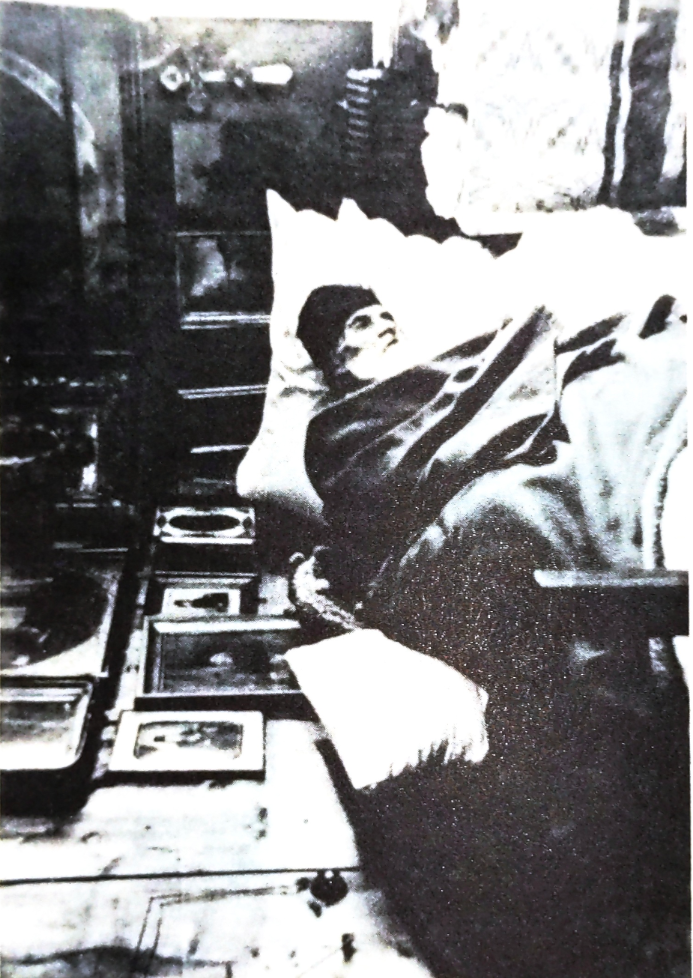
\includegraphics[width=4.25in]{./Images/Elder_Joseph_Bed.png}

	The Elder Joseph shortly before his repose
\end{center}
\vspace*{\fill}\restoregeometry
\titleformat
	{\part} % command
	[display] % shape
	{\bfseries\Large} % format
	{
		\begin{center}
		\thepart
		\end{center}
	}
	{0.5cm}
	{
		\vspace{-1.5cm}
		\begin{center}
			\color{red}
	} % before-code
	[
			\color{black}
			\vspace{1cm}
			\bfseries\normalsize		
			The poor offering of a spiritual son to the\\memory of an unforgettable Father\\
			\vspace{2cm}
			{
\includegraphics[height=5cm]{./Images/Part_Emblem.png}}
		\end{center}
	]
	
\part{The Life\\of the Optina Elder\\HIERO-SCHEMAMONK JOSEPH}

\newpage
\begin{center}
	
\includegraphics[width=\the\textwidth]{./Images/Chapter_Banner.png}\\
	\vspace{1.5cm}
\end{center}
\hugered{A}FTER THE REPOSE of Batiushka Fr. Joseph, I began to receive many letters from relatives, acquaintances, and persons completely unknown to me--all with one and the same request: to describe to them in greater detail the final moments and the burial of Batiushka, and to relate what was known to me of his biography. These letters became so many that, having answered two or three letters with haste, I suddenly felt utterly unable to satisfy everyone with my answers--a fresh wound is still too sensitive. The inevitable contact with recent sorrowful events through their recounting in my letters called forth memories too painful for my heart. The thought that was looming within me, to leave unanswered the letters which I had received, was quickly dispelled by pangs of conscience. I thought to substitute for the letters some short publications concerning the life and repose of Batiushka, but unfortunately, other than ``The Sermon at the Grave'' (in its printed form quite different from that in which it was spoken at Batiushka's burial), and a very brief article conveying nothing either to the heart or to the mind--apart from these nothing printed concerning Batiushka had appeared!

Whereupon, having taken a blessing at his dear little grave, I decided to relive once more in my soul the grievous loss, and by means of the printed word to answer the inquiries of all who had turned to me. By this I hoped, first of all, to satisfy their desire, which I understood so well, to know something of the life of the beloved Elder. And, secondly, I wished to honor with my own contribution, however small it might be, the dear memory of him by whose kindness and encouragement in the course of so many years I, the worst of his spiritual children, had profited.

Batiushka was born on November 2, 1837, in the village of Pokrov of the Starobelsk District of the Kharkov Province. His parents, Evfimy and Maria Litovkin, were very pious people who tried to raise their children in the fear of God. There were six children, three daughters and three sons, of whom Batiushka was the middle child.

Evfimy Litovkin was from a well-to-do peasant Cossack family. For a long time he had held the position of village-head and enjoyed the respect of all, Maria was from a family of the clergy. Both very much loved to help the poor, and often did this without the other's knowledge. They especially venerated Saint John the Almsgiver, in whose honor Batiushka had been named.

Batiushka's father secretly desired that some one of his children enter the monastic life, and the Lord fulfilled this desire in the person, firstly, of his daughter Alexandra, and later also in the person of Batiushka. (His daughter Alexandra entered the Borisovsk Women's Hermitage in the Kursk Province. She led an exalted spiritual life, even served as an Eldress, and reposed as a schema-nun with the name Leonida.) Batiushka loved to recall his childhood, and himself would relate how on feast days his mother would wake all the children for Matins, and after returning from church, between Matins and the Liturgy she would make Batiushka read an \textit{akathist} aloud, while she herself censed throughout the house. Batiushka would say, ``Ooh! She was strict! She was more like a man than a woman.''

Concerning his father Batiushka would say that he was, on the contrary, of a lenient character and was reluctant to punish the children. When Mother Leonida, at the beginning of her monastic life, was subjected to great temptations and thought of leaving the convent, her mother, who had just reposed, appeared to her during sleep and sternly reproved her, reminding her of her monastic vows.

When Mother Leonida told Batiushka Fr. Amvrosy about this, he said to her, ``Your mother is a saint!''

Batiushka's father reposed in 1841, and in 1848 his mother reposed from cholera. Batiushka himself related to me that she was the first in their village to die from this epidemic and the first to be buried in the farther cemetery.

Being left an orphan, Batiushka had to undergo and endure much that was grievous, first from his older brother and later from various masters for whom he worked. Moving from one city to another, and traveling the distance between them on foot, Batiushka endured both hunger and cold. How many times in the inclement autumn weather his feet were soaking wet and frostbitten, and he ate nothing for several days at a time.

Once, being exhausted by the long walk and by hunger, Batiushka entered a certain village; at the entrance to the village, two Cossack women were selling bread. One of them caught sight of the exhausted and scrawny young wayfarer; her sensitive heart was filled with pity, and turning to her friend, she said, ``The poor one! He's probably hungry; let's give him some bread!'' and with these words she gave Batiushka a hot soft roll. In relating this incident not so very long ago to one nun, Batiushka said that to the present time he remembers with thanksgiving those kind women and what they did for him. The compassionate Cossack women, to whose lot fell the good fortune of showing such a kindness to the future great Elder, did not even suspect that by this act of almsgiving they had perhaps entrusted themselves for eternity to his holy prayers for their salvation.

Batiushka found himself in Taganrog and in Rostov; he worked in the tavern of an Armenian in Nakhichevan, and finally wound up at the mill of a certain pious old miller who loved to attend the church services and to read spiritual books, and he never hindered Batiushka from doing the same. From childhood Batiushka loved church, and wherever he lived, on feast days he always tried to be at the Liturgy; hence, his life at the mill was much to his liking.

From there he thought to go to Kiev to venerate the saints of God who repose there, but on the way he stopped at the Borisovsk Hermitage to visit his sister. She persuaded him to go first to Optina and provided him with letters to Batiushka Fr. Amvrosy who had just then entered upon the struggle of eldership after the death of his guide, Batiushka Fr. Makary.

Batiushka Fr. Joseph went to Optina in 1861 on the first of March, ``On Evdokia'' (i.e., on Saint Evdokia's day), as Batiushka would often say. In accord with the counsel of the Elder, he remained at Optina where he was straightway received into the brotherhood of the skete and put to work in the skete kitchen where he remained until Trinity Day.\trans{The Sunday of Pentecost.}

On this day, which was to be significant for him, he was appointed as cell-attendant to the Elder Batiushka Fr. Amvrosy and from that time he spent thirty years inseparable from his great teacher and father.

Batiushka's pious attachment to Fr. Amvrosy was most moving. Batiushka always spoke of him with a smile of tender compunction, and when it happened that you would ask his help and holy prayers in some important matter, he would often advise, ``And you ask Batiushka, too!'' In his instructions also he loved to cite the words of his departed Elder.

Concerning Batiushka's life as cell-attendant for the Elder Amvrosy I know little, but I have heard from many that as a cell-attendant he was irreplaceable. Always distinguished by his extraordinary accuracy and precision in fulfilling his duties, Batiushka always related the Elder's answer word for word to those who made inquiries through him, for which cause the nuns who came to the Elder especially loved him, and if it was difficult to get to the Elder, infirm and burdened as he was by the multitudes of people, then they would summon Batiushka and through him receive the most precise answers. Likewise, many turned to Batiushka Fr. Amvrosy by writing letters which were presented to him by Batiushka Fr. Joseph, who faithfully conveyed Batiushka's answers to all the points of each letter.

Batiushka was always distinguished for his reserve and silence in dealing with visitors, and unless he found it absolutely necessary, he would rarely go out to the people in the hut. In 1884, Batiushka was ordained hieromonk, and from that time on Batiushka Fr. Amvrosy began to send the nuns to him for confession.

When Batiushka was still a hierodeacon, Fr. Amvrosy blessed several nuns to turn to him in order to profit by his counsels. One of them related that in order to verify what had told her by Batiushka Fr. Joseph, she afterward asked the Elder concerning the same matter, whereupon Fr. Amvrosy told her exactly the same thing as had Batiushka. In this manner, Fr. Amvrosy was preparing Batiushka to succeed him as Elder.

In 1888, Batiushka fell dangerously ill with typhoid; he was tonsured into the schema and he prepared for death. Once, when it was especially difficult for him, he sent the cell-attendant who was looking after him to Batiushka Fr. Amvrosy with a request to allow him to depart in peace. When the cell-attendant related this message to Batiushka Fr. Amvrosy, the Elder said, ``Go to his cell and say nothing to him, but say to yourself: 'Holy, Holy, Holy, Lord of Sabaoth; heaven and earth are full of Thy glory.''' The cell-attendant returned to the infirmary, entered Batiushka's cell, and fulfilled what had been commanded by the Elder. As soon as he had pronounced the last word, Batiushka, who was lying behind a screen, rang and asked for tea. He drank three cups, and from that day on he began slowly to recover. Batiushka himself related this to me.

I have heard from many that during this illness the Heavenly Queen had appeared to Batiushka, but on account of his humility Batiushka concealed this. A certain nun who had been speaking with Batiushka Fr. Amvrosy concerning the Mother of God had said, ``Surely the Heavenly Queen was very beautiful,'' to which Batiushka Fr. Amvrosy had said to her, ``Why don't you go and ask Fr. Joseph what she was like in old age?'' The nun went to Batiushka with this question, but he declined to answer.

In the period of his independent eldership, Batiushka Fr. Joseph, as long as his strength held out, received and confessed everyone, not refusing a single person. He himself would read the confession booklet for those who were illiterate. Once, in the first week of Great Lent, I was startled at seeing the multitude of people who had come for confession, who had filled both the men's and the women's huts to overflowing. How could weak little Batiushka hear everyone's confession completely? Such a mass of people--it was totally beyond comprehension! One can only explain it as the grace of eldership.

In the first week of the Great Fast almost everyone at Optina without exception was preparing to confess and to receive Holy Communion: the brethren of the monastery as well as those of the skete, the nuns at the livestock compound, and everyone living in the monastery. At that time they all confessed to Batiushka, and this did not include the Shamordino sisters and the pilgrims who had come, the flow of which is especially great during this week.

It would happen that by prior arrangement with Batiushka you would go confess after Matins, about six in the morning, and Batiushka would already have been hearing confessions for a long time, sitting on his little bed in the reception room with a pillow behind his back.

How simple and yet how sublime was this confession in its mystical nature! You would read the booklet for confession and tell the sins which you had written down in order to remember them, and it would seem you were all set. However, in actuality, this was far from the case. While you were recounting your failings, Batiushka in a half-whisper would slowly say the Jesus Prayer, and at the same time you would clearly feel that at each prayer, Batiushka's prayerful sigh was ascending to the Lord. From this, such peace would be felt in the soul of the sinner who had just been cleansed, such spiritual joy, that only he who has even once been deemed worthy to confess to the holy Elder is able to understand completely. Then he would read the prayer of forgiveness.

With what humility Batiushka would read the words of this prayer! This humility did not even escape the nine-year-old spiritual son of Batiushka who had confessed to him from the time he was six. On his way home one time after confession he said to me with such delight, ``That Batiushka! When he reads the prayer of forgiveness and says, 'And I the unworthy...' he says these words with such feeling, as if in truth he were unworthy!''

Humility was a distinctive characteristic of Batiushka's soul, and he tried to teach this virtue to his spiritual children. Often his entire instruction consisted of two admonitions: ``Humble yourself! Be patient!'' And if you said, ``Batiushka, I don't know how to be humble!'' Batiushka would answer, ``Reproach yourself!'' (i.e., for not knowing how to be humble). And this new instruction implied what he had said before, ``Humble yourself!'' If you were to ask Batiushka to speak a word of profit, it was rare that you would hear anything else; almost always one and the same: ``Humility, and patience, and deliverance from... here Batiushka would name a passion.

One time, when I was lamenting my lack of correction before Batiushka, I chanced to touch upon this lack of correction in another person. With a gentle reproach he said to this, ``The saints considered themselves worse than all, yet we are better than all!''

In all things Batiushka made use only of that which was most essential, and he did not bless others to have anything beyond what was necessary. Before Batiushka's namesday one of his spiritual daughters asked for a blessing to sew him a new cassock for the occasion. Batiushka said, ``What for? After all, I already have one. And it's sinful to have more than you need.''

Another time, I asked for a blessing to request that the floors in my rooms be painted and the walls whitewashed. Batiushka asked, ``What? Is it so dirty that it's impossible to live there?'' I said that one could live there, of course, but that the floors were worn down. Batiushka said, ``That’s vainglory!'' Batiushka did not even once fix up his own cell in which the Elder Fr. Amvrosy had struggled for more than thirty years and in which he himself had lived for another twenty years, although it needed it, since with the passage of time the ceiling had become sooty. One might rightly say of the furnishings of this little cell, sanctified by the fifty years of ascetic struggles of the two great Elders, that they are of such simplicity that just to look at them brings one to compunction.

Batiushka was very sympathetic to people's needs and sorrows. In answer to a letter sent to me from a certain acquaintance who had lost two children from diphtheria, Batiushka said a few words of consolation and then added, ``Whatever you say to comfort them, still it's not easy to lose two children!'' So much concern and understanding of this grief was conveyed in Batiushka's voice that I was amazed at how Batiushka could sympathize with him, he being a stranger to the worldly joys of a family!

Every day at noon, the poor would gather in crowds on the porch of the hut and the cell-attendant on duty would give them all alms, and to those whose parish priests had given them a note attesting to their inability to work, or concerning a particular need of the petitioner, an even greater amount would be given. Last year at the command of the superiors, the distribution of alms was carried out twice a week in order to avoid the continuous presence of poor people in the monastery and the frequent incidents of robbery which followed in consequence of this. When I chanced to tell Batiushka of one attempted robbery by a poor girl, Batiushka became pensive and, with a voice filled with sorrow, said, ``Ah, poverty!''

At Christmas and Pascha, Batiushka would receive whole stacks of letters and postcards with requests for assistance on the feast. Batiushka answered each of them with a short greeting for the feast, a wish for peace and a blessing, and included a contribution of money. Once, when his secretary was ill, Batiushka entrusted me with addressing the envelopes of my own replies to these letters, and for the addresses he gave me a large packet of postcards which he had received. I drew Batiushka's attention to the fact that many letters were written by one and the same hand. Batiushka, laughing cheerfully, said, ``Yes, they are all written by the same hand!'' Then he added affectionately and submissively, ``Well, God be with them. They are the poor!''

On the twelve Great Feasts, Batiushka served the Liturgy in the monastery, taking part in the late concelebrated Liturgy. With what joy you would await the solemn moment when, having taken off his vestments after the completion of the Liturgy, the radiant Batiushka would appear from the door of the left side of the church, smiling, radiant with an other-worldly and graced-filled joy from mystical communion with his beloved Lord! Monks and nuns and lay people from every calling and position surrounded the holy Elder in a dense crowd, trying to receive his blessing, to greet him for the feast, to give him a small \textit{prosphora} which had been offered for his health, and to be deemed worthy to be entrusted with the pleasant task of carrying Batiushka's \textit{mantia} back to the skete.

A multitude of hands stretched out for it, but this good fortune most often fell to the lot of a certain pious old woman, T. G. A., who lived at Optina--a woman of prayer and an ascetic, who later reposed in the schema. She, having seized the precious burden, breathing heavily from joy and also from a weak heart, hurried at a run along the straight path in order to arrive at the porch of the hut before Batiushka. Meanwhile, Batiushka, giving his blessing left and right, with difficulty made his way through the crowd of people to the carriage awaiting him at the gates of the church wall, accompanied always by the moving exclamations of the crowd, ``Dear Batiushka!'' ``The dear little saint of God!'' ``Our own dear Father!''

Batiushka served for the last time on the feast of the Dormition in 1905, and from the sixteenth of August he began to complain of weakness which did not leave him all autumn, and which grew worse before it finally let up. On the ninth of October, the eve of the memory of Batiushka Fr. Amvrosy, Batiushka felt so ill that he was unable to receive visitors and to confess the many Shamordino sisters preparing to take Holy Communion on the day of Batiushka Fr. Amvrosy's repose. But some two days later, he again began to receive visitors in spite of his weakness.

On the eve of the twenty-fourth of October, Batiushka became so weak from over-exhaustion that he almost died; they gave him Holy Unction that night and gave him to partake of the Holy Mysteries. The doctor who was called on the following day diagnosed chronic exhaustion due to his terrible anemia, but consoled us with the words, ``Batiushka has the heart of a young man.'' He prescribed complete rest for the course of a prolonged period of time and an improvement in his diet.

From this time on, Batiushka was unable to hear the confessions of such a multitude of people and he entrusted the Shamordino sisters to another spiritual father. He continued, however, to confess the brethren himself for yet another half a year. In April of 1906, Batiushka fell ill a second time with acute influenza, and when on the ninth day of his illness his temperature fell, he grew so weak that arrangements were made to allow him to bid farewell to the brethren and any others who so wished. The doctor from Kozelsk who came in the evening ordered that this parting be discontinued, saying that although Batiushka was weak, yet he had a good heart, and if he were allowed complete rest, and if he were given some food to strengthen him (Batiushka had not tasted any food for eight days), then there was yet hope for his recovery.

The parting was discontinued, the hut locked up, and Batiushka began, albeit slowly, to recover. Only in a month's time, on the twenty-eighth of May, did Batiushka come out for the first time to give a blessing to the people in the hut. This joyous occasion will never be forgotten! When Batiushka, emaciated, but happy and cheerful, illumined with his wondrous smile, appeared in the doorway, supporting himself with a cane, all understood in a moment that clearly he was in truth risen from the dead, and what a feeling of gratitude toward the Lord overflowed the hearts of those present at the sight of this evident mercy of God.

The Lord had had mercy on us once again: yet again and for the last time, He had preserved the Elder's life which was precious to all. It was in February of 1909 that the third critical illness overtook Batiushka. It was so serious and painful that a doctor was summoned from Moscow. This time the doctor from Moscow marveled at the good condition of Batiushka's heart despite his advanced years. Batiushka himself later told me that this was because, from his youth, he had never drunk wine and had never taken any medicines, except homeopathic ones.

After each of these grievous illnesses Batiushka would say, ``You see? I should have died, but the sickness left in answer to their prayers!''

After his illness in 1906, on account of his weakness Batiushka could no longer carry out his duties as skete Superior, which was a position he had occupied for twelve years, enjoying the pious love of the skete brethren. He resigned from it, as also from his duties as spiritual father, and would confess only a very limited number of disciples. In these last five years of his life, Batiushka became very weak. Often he had to discontinue the reception of visitors for several days at a time, and sometimes for an even longer period of time; the reception of visitors very much exhausted him.

Toward the end, beginning with the new year of 1911, Batiushka grew especially weak, and for the whole of February he received almost no one. S.V. Perlov's repose, followed by that of Matushka Abbess Catherine and the sorrowful conditions at Shamordino resulting from these two losses, all the more shook Batiushka's health. Batiushka would never complain of any pains, but often said that he felt an extraordinary weakness. In spite of this, Batiushka forced himself to go out to the reception room, and during the passage through the corridor from his cell, he would hold onto the wall with his hand. Having conversed with two or three people, he would have to go back to his cell and lie down since he felt dizzy and was completely exhausted. To the cell-attendant's request that he give himself some rest and not receive visitors, Batiushka answered, ``It will be on my conscience if I do not receive them,'' and having taken a short rest, he rang and asked, ``Well, who else is there?''

Lying in his cell in the intervals between his going out to the reception room, Batiushka continuously fingered his prayer-rope and said the Jesus Prayer in a whisper. In order to avoid being deceived in the number of prayer-ropes which he had said, Batiushka would keep track of them with olive pits; one could always see on the small table at the head of his bed a little box with these pits.

Batiushka had always been very temperate in his eating, and from December on he could not even eat his customary scant fare, for due to the weakening of his entire system his stomach had also grown weak, and Batiushka began to experience pain in the pit of his stomach even after fish soup.

Batiushka's unchanging daily fare consisted of \textit{shchi} (cabbage soup), this being made from fresh cabbage or from sauerkraut, water, and a very small amount of sunflower oil. This was made without mushrooms, which Batiushka's stomach could in no wise tolerate. With the \textit{shchi} they would give him fish soup or oatmeal gruel\trans{Literally, ``Hercules soup.''} made with water, and on non-fast days he had two soft-boiled eggs, of which Batiushka ate only the yolks. For dinner on non-fast days, they boiled milk for Batiushka, which he had with a piece of white bread, and on fast days they made watery rice \textit{kasha} (porridge) with almond milk. Such it was day after day, year after year, without change, without the slightest variation! Whenever anyone advised Batiushka to try some sort of nourishing food, Batiushka would try it and say, ``Somehow it doesn't suit me,'' and he would return to his former customary diet.

On the third day of Pascha, the twelfth of April, Batiushka fell ill with the illness from which he died. It began with acute vomiting and then an increase in his temperature to 102.4° F. Batiushka utterly refused to summon the doctor or to take any medicine, in spite of the persistent requests of all his spiritual children. Nevertheless, the doctor was called for at the request of the Shamordino benefactress, A. Y. Perlovaya, who had gone to the Fr. Archimandrite with her request, and out of humility, as if taking it as an obedience, Batiushka agreed to receive the doctor. He arrived on the seventh day of the illness, diagnosed malaria, and found that Batiushka's heart was very weak, and therefore that there was little hope for his recovery.

Batiushka remained ill for four weeks. His temperature would rise and then fall, only to rise and fall again. Batiushka was tormented by thirst; the inside of his mouth had completely dried up because of the fever, and Batiushka often asked for something to drink, but then he would drink only water. Sometimes he would tell the cell-attendant to add a few drops of homeopathic medicine to the water.

Batiushka received Holy Communion daily.

On the twentieth of April, Batiushka desired to bid farewell to the brethren, and he gave a blessing to send word to Shamordino that the sisters be given leave to come.

There began a sad and moving spectacle which continued for several days in a row. The sisters in groups of fifteen or twenty, one after the other, entered Batiushka's cell, prostrated themselves to the ground, and silently kissed the dear hand with which he blessed them, and scarcely able to restrain their weeping, they left his cell. Batiushka looked upon all with his eyes, now filled with sorrow and suffering, and appeared to recognize each one. In alternation with the sisters, there were also allowed to enter all the lay visitors at Optina who wished to bid farewell to the departing Elder. After each group of sisters, short intervals of half an hour to an hour were made, depending on how Batiushka was feeling. When Batiushka was asked to stop the bidding of farewell for a longer period of time, Batiushka did not agree and he hastened in order that everyone be allowed to come the sooner. On two occasions during this time, Batiushka's clairvoyance was unexpectedly revealed. On the twenty-third of April, at five o'clock in the evening, the skete Fr. Superior asked Batiushka if he wouldn't prefer to stop the sisters from coming. Batiushka answered, ``They want to come; if they do not, they will be grieved!'' and he gave a blessing for a telegram to be sent to the Mother Superior at Belev so that she would allow her sisters to come to Optina in groups. On the very same day and hour at Belev, a certain nun who was devoted to Batiushka asked the Mother Superior if she could go to Optina to bid farewell to the Elder, but Matushka answered that she had not as yet received any instruction about allowing the sisters to come, and she refused to let her go. At ten o'clock in the evening, Batiushka's telegram was received, and on the following morning that nun went to Optina on the early train with the first group of sisters who had received permission to come. When she went in to Batiushka, he recognized her, stared at her, and giving his blessing, said, ``Matryona.''\trans{``Matryona'' is the diminutive form of ``Matrona.''} The other instance was the following: On the twenty-fourth of April, at about four o'clock in the afternoon, Batiushka asked, ``Are there nuns from Sevsk here?'' The doctor's assistant who was on duty that day went out into the hut and asked if there were any nuns from Sevsk, since Batiushka was asking for them. There were none, but in an hour three nuns from Sevsk came to Optina. Batiushka had foreseen their arrival.

With each passing day, Batiushka was failing noticeably; his dear face became all the more strained, his nose became drawn, and his little eyes sank deeper and deeper. His weakness so increased on the last two days that Batiushka did not have enough strength to cough up the phlegm which tormented him terribly in the mornings, especially on the morning of his repose, and Batiushka, groaning, made incredible exertions to be freed of it, after which he would feel extreme fatigue. At the offer of the cell-attendant that he drink a little hot tea, in order to wet his throat and alleviate the discharge of the phlegm, Batiushka replied in exhaustion, ``What do I need tea for now?'' At eight o'clock in the morning, Batiushka took Holy Communion for the last time, and after Communion he said to those near him, ``Pray that the Lord release my soul from my body.'' At about two o'clock in the afternoon, Batiushka began suffering from a terrible chill. Batiushka raised himself up a little on his bed but at the same moment told the cell-attendant who was with him to lay him down again, but the cell-attendant could in no way do this: Batiushka had become cold and stiff; his back would not bend, and his little hands and feet and his whole body shivered from the terrible chill. This quickly turned to fever, however. His members straightened out, became soft, and Batiushka could be laid down and covered up. After this, Batiushka lay peacefully until his repose; at about five o'clock he said quietly, ``Icon,'' expressing his desire that an icon be placed near him. They brought the icon of the Mother of God with which Fr. Archimandrite Isaaky had blessed Batiushka, put it opposite Batiushka, and later transferred it to the table by his pillow and lit a candle before it.

From that time on, Batiushka began to grow extremely weak; his little eyes would no longer open, and Batiushka said nothing. At eight o'clock, they began to read for Batiushka the Prayers at the Departing of the Soul, and gathered the brethren and the people in charge. After the prayers, they let us in to say farewell. Batiushka lay on his back; his head was propped up high; his little eyes were closed; his face was bright with an expression of complete rest; his half-opened mouth drew in air at every breath with difficulty. Batiushka had on a white flannel shirt and his \textit{paraman};\footnote{See Glossary, p. 298.} his legs up to the waist were covered with the same grey cassock which Batiushka had customarily worn throughout his life. On his chest lay a shroud with relics of the holy Great Martyr Barbara; in his right hand was a small white wooden cross. I made a prostration and carefully kissed his dear little hand several times, in my mind bidding farewell to Batiushka who, without a doubt, was now departing, and going aside to the table, gazed for a long time at his dear face, as those who had come after me were saying farewell. His little face reflected tranquillity, and there was no trace in it of the earlier expression of suffering. When all had bidden farewell, we were told to leave. Afterward the cell-attendant Fr. Z., and Fr. D. of the hospital, who were present at Batiushka's repose, told me that Batiushka had had an extremely peaceful repose; there was neither fear, nor any alarming movements of his limbs. As soon as Batiushka had turned his dear head to the right side for a moment, he took a look, again turned away, and closed his little eyes.

Batiushka's breathing became shallower, and finally, he frowned slightly and swallowed something, after which his breathing stopped, and Batiushka's holy soul departed its earthly dwelling, belabored with the ascetic struggles of fifty years. This was at a quarter to eleven in the evening. Batiushka reposed with his little eyes half-open; Fr. Z. closed them with his own hands.

Two \textit{pannikhidas} were immediately served, after which they prepared Batiushka, clothed him in the schema, and laid him again on the bed on which he had reposed.

\textit{Pannikhidas} were served right up until morning. At about six in the morning, they placed Batiushka in the coffin and brought it out to the skete church for the Liturgy.

At 10:30 in the morning, after the late Liturgy at the monastery, the funeral toll sounded in the skete and the procession moved out of the monastery along the path to the skete. After the celebration of the \textit{pannikhida} served by all the clergy, they began to carry him out. This bearing out of Batiushka with the sad sounds of the tolling of the bells reminded one of the procession with the Lord's shroud on Great Friday. The white vestments of the clergy, the marvellous, sunny weather, and the great crowd of people gave this bearing out an aspect of joy and triumph. They carried Batiushka around the old church of the skete in honor of Saint John the Forerunner and brought it out along the straight path, past his cell, through the \label{holy-gates}Holy Gates into the monastery, which were not yet reached when the procession was met with the tolling of the monastery bells. They brought Batiushka into the Church of Saint Mary of Egypt, at first before the main altar, and all the clergy together participated in the solemn \textit{pannihkida} which was immediately served. After this, continuous \textit{pannikhidas} were begun due to the zeal of the hieromonks, and they were served continuously all that day and every day following until Batiushka's body was given over to the earth, and even then one \textit{pannikhida} followed another.

For me, this was a genuine consolation; it was even something of a joy to stand at Batiushka's grave listening to the sound of the prayers being offered for his righteous soul. The chanters all the while took turns, first our monks, then those of the skete, then the Shamordino sisters, then those of Belev. All the time people were placing small crosses, icons, belts, prayer ropes against Batiushka's body; on the day of the burial, when Batiushka had already been brought into the church, Batiushka's coffin was literally covered over with these things, which their owners recovered with great faith and piety. I was deeply moved by a poor little boy who placed on Batiushka's little hand a small copper cross on a pink paper ribbon, and then piously made the sign of the Cross and kissed Batiushka's little hand. On each of these days, at the request of the nuns and of those who revered Batiushka, the hieromonks lifted up the cloth and revealed Batiushka's dear face. Batiushka was as one alive, so comely, radiant, peaceful, only very, very thin. On the eleventh of May, the third day after his repose, when the deceased are usually given over to the earth, I and several others noticed that Batiushka's dear face had become darker since the morning, but on the twelfth of May it again became bright and more radiant than before. During all those four days, not even the slightest odor could be sensed from Batiushka's body. A small sign of corruption showed before the burial only on his hand, at the place where we had touched him with our sinful lips when we kissed him, and that the size of a three-kopeck copper coin; above that spot, however, under the schema his hand was completely white. It is remarkable that his little hand was soft and warm, much warmer than when he was ill, and hieromonk Fr. D., having put a second pillow under Batiushka's dear head so that his face would be higher, said that all of Batiushka's body was soft and not stiff, as is usually the case with the bodies of the deceased. On the eleventh of May, there was performed in the church a solemn vigil for the deceased, after which they closed the monastery until three in the morning, and we had to leave.

From three in the morning, \textit{pannikhidas} were again begun until the early Liturgy, which was celebrated right there in the church in the side chapel of Saint Nicholas. During all that time, until the late Liturgy, and even during it, the people did not cease to come up to kiss Batiushka. At the end of the late Liturgy, which had been magnificently served by three Archimandrites and a large number of hieromonks and parish priests, the proctor, Fr. Theodot, gave a sermon on the reposed Batiushka. This sermon, in which the basic traits of dear Batiushka's character were so faithfully expressed, was infused with such warmth, such sincere love for the reposed, that it warmed the sorrowing hearts of those present and filled them with a feeling of joy.

I do not know which of the services was the most solemn and majestic, but all in general reminded one more of the ``uncovering'' of holy relics, than the ``covering'' forever of our dear Batiushka from the loving gaze of his spiritual children. Many, coming away from the grave, expressed aloud this very impression. In the crowd one heard several times the compunctionate words, ``Holy relics!''

There were several instances of miracles which took place at Batiushka's grave. One of them I recall as especially worthy of credence. A certain peasant woman had for some time been suffering from some unknown disease which defied diagnosis, for which she had spent much for treatments, but received no benefit. As soon as she kissed Batiushka's little hand, she began to scream and struggle. After Batiushka's burial, she and two companions passed by Batiushka's grave on their way to Fr. Anatoly, and I myself saw how, as they approached the grave, she suddenly began to be obstinate and to quietly cry out, ``I won't go! I'm afraid of him, afraid!'' Her companions took her by the arm and tried to move her from the spot but she wouldn't budge; then they dragged her with difficulty to the grave and threw her down on the fresh mound of earth. The woman immediately grew quiet, and having lain there a little, got up and crossed herself. Praying for a while at the grave, she continued on her way in peace. In the evening, I again saw how she went up to the grave in complete tranquillity, prayed and thanked Batiushka aloud, and then, turning to me and to the two nuns who were there also, told us of her former terrible illness and grief, and ended her account with the words, ``But Batiushka here disclosed my illness.''

Two other instances happened on account of the belts which were brought from Batiushka's grave on the very day of his burial to two sick women, and they received alleviation from their sufferings as soon as they had put them on.\footnote{These instances were recorded and submitted to Shamordino for inclusion in the detailed life of Batiushka Joseph which is being compiled there.}

The Lord glorified Batiushka with the gift of healing even during his lifetime. How many instances there were wherein, at the touch of Batiushka's hand to the ailing place or by his making over it the sign of the Cross, and frequently at one word of his alone, ``Help, O Lord!'' headaches and toothaches as well as other human infirmities subsided.

How much more was this true in the case of spiritual turbulence and sinful states of soul! A person tempest-tossed by them had only to stand before Batiushka, to feel upon himself his meek prolonged glance, or an affectionate strike of his hand on the head, when all that was raging in the soul immediately disappeared, and you would be so filled with such peace, such joy, that you could only wonder whither the oppression of sin which had hitherto exhausted you had fled and gone. And you would clearly feel at that moment that this oppression of sin is not an inherent characteristic of the human soul, just as physical illness is not a property of the body, but something alien, foreign, being from without and concealing itself instantly at the first rays of God's grace.

Before his repose, the Elder Fr. Leonid said to many, ``If I receive God's mercy, my body will become and will remain warm.'' And Batiushka Fr. Amvrosy said, ``When I die, then for glorification on earth, my body will decay.'' And, in truth, Batiushka Fr. Amvrosy did decompose quickly.\trans{The sweet fragrance that comes forth from the holy relics of the saints--and oftentimes, from the remains of the newly-reposed--is considered an indication of sanctity, inasmuch as the saints and all who are pleasing to God have become Christ-like and their lives and prayers have become as it were a whole-burnt offering and fragrant incense offered unto God (cf. Ps. 140:2; Eph. 5:2; Rev. 5:8). In connection with the Elder Amvrosy's prediction, see John Dunlop's \textit{Staretz Amvrosy}, p. 119, where it is pointed out that although ``a heavy death-like odor'' was quickly sensed after his repose, as the Elder Amvrosy had himself foretold, yet this diminished with each passing day, so that by the third day, despite the stifling heat in the church, ``a pleasant smell like that of fresh honey began to come forth from the body.''}

Batiushka Fr. Joseph's humble reserve made him inaccessible to the understanding of many people, and therefore not everyone valued his grace-filled qualities. Not infrequently, one heard such words as, ``What's wrong? He doesn't say anything!'' or, ``He speaks so little and never foretells anything!''

The words cited above concerning the causes of incorruption were spoken by the great luminaries of Optina eldership, chosen by God Himself as mediators between Him and sinful people. They spoke only the truth and one would be in error to disbelieve their words. From these accounts, one cannot but be confident that Batiushka Fr. Joseph, having partaken of earthly glory, has received after death a greater glorification, in Heaven and on earth! In Heaven, his most pure soul has been glorified by receiving ``the crown of goodness from the hand of the Lord,'' and on earth his much-laboring ascetic body, which patiently endured so much, has been glorified by incorruption and has become a well-spring of mercies for those who flee to him.

From childhood, Batiushka's whole life was passed in the midst of sorrow and privation which he endured to an amazing degree without complaint. They did not leave him even at the end of his life. During his last four years, Batiushka had to endure great troubles. To bypass this in silence would be a great omission in the biography of Batiushka, since it was precisely in this that there was revealed all the greatness of his spirit, all his truly evangelical meekness with which Batiushka met the grievous offences brought against him.

The words of the Saviour, ``Learn of Me, for I am meek and lowly in heart,''\footnote{Matt. 11:29.} could very well serve as an epitaph for the entire life of Batiushka.

Truly the Lord Himself, by His own example and teaching, has encouraged us to imitate Himself, and Batiushka was an exact fulfiller of the law of Christ. Wherefore, I shall not err, I think, if I end my poor lines concerning him with the words: Come unto him, to his holy grave, all ye that labor and are heavy-laden; sigh unto the Lord that He grant rest to his righteous soul; make known to him, as to one living, your sorrows; and truly ye shall find rest for your souls, even that rest and peace which so abundantly was poured out during his lifetime on all who with faith came unto him.


\addcontentsline{toc}{chapter}{APPENDIX A\\The Cell Rule Of Five Hundred Of The Optina Monastery}
\chapter*{The Cell Rule Of Five Hundred\\Of The Optina Monastery\footnote{This Cell Rule is taken from \textit{The Monastic Cell Rule} (in Russian), reprinted by the Convent of the Vladimir Mother of God in San Francisco (San Francisco, 1977), pp. 23-27.}\markboth{Appendix A}{}}

\label{cell-rule}\hugered{I}n addition to the church services: the Liturgy, Matins, and Vespers with Compline, which all of the brethren of the monastery are obliged to attend, many of them daily read in their cells: One chapter from the Gospel in order, beginning first with the Gospel of Matthew, to the last chapter of the Gospel of John, and two chapters from the Epistle, likewise in order, beginning with the Acts of the holy Apostles and ending with the last chapter of the Apocalypse of Saint John the Theologian. The last seven chapters of the Apocalypse are read one a day. In this way the last chapter is read on exactly the same day as the last chapter of the Gospel of John.\footnote{There are 89 chapters in the 4 Gospels, 171 chapters in the remaining books of the New Testament. With the 7 concluding chapters of the Apocalypse being read one a day, there would be 89 readings, corresponding to the chapters of the Gospels. One would thus begin a new cycle every 90th day. -TRANS.} Then, after the completion of the reading of the whole New Testament, in this manner they begin again from the first chapters a new cycle of reading in precisely the same order. From the Psalter they read one \textit{kathisma} a day, beginning with the first and ending with the last.\footnote{There are 20 kathismata in the Psalter. -TRANS.} In addition to this, they perform the so-called Cell Rule of Five Hundred in the following order:

After the customary three prostrations performed at the commencement of every rule of prayer, both in church and in one's cell, with the prayers: (1) \textbf{God, be merciful to me a sinner.} (2) \textbf{God be gracious\footnote{The Slavonic word \textit{ochisti} is often translated “cleanse,” because the word in Slavonic has the fundamental meaning of “cleanse" or "purify.” An extended meaning is the cleansing of sins, which includes meanings of “to forgive," "to show mercy,” “to be gracious.” This last rendering accords with the Greek \textit{hilastheti}. –TRANS.} unto my sins and have mercy on me.} (3) \textbf{O Thou Who hast fashioned me, Lord, have mercy. I have sinned beyond measure, O Lord, forgive me,} in one's cell a fourth prostration is added together with the prayer: \textbf{My Lady, Most Holy Theotokos, save me a sinner.} Then the following prayers are said:

\begin{center}
Through the prayers of our holy Fathers, Lord Jesus\\Christ our God, have mercy on us. Amen.

Glory to Thee, our God, glory to Thee.
\end{center}

Heavenly King, O Comforter, the Spirit of truth, Who art everywhere present and fillest all things, O Treasury of every good and Bestower of life: Come and dwell in us, and cleanse us from every stain, and save, O Good One, our souls.

\begin{hangparas}{.25in}{1}
Holy God, Holy Mighty, Holy Immortal, have mercy on us (3).

Glory to the Father, and to the Son, and to the Holy Spirit, both now and ever, and unto the ages of ages. Amen.
\end{hangparas}

All Holy Trinity, have mercy on us. Lord, be gracious unto our sins. Master, pardon our iniquities. Holy One, visit and heal our infirmities for Thy name's sake.

\begin{center}
Lord, have mercy (3).
\end{center}

\begin{hangparas}{.25in}{1}
Glory to the Father, and to the Son, and to the Holy Spirit, both now and ever, and unto the ages of ages. Amen.
\end{hangparas}

Our Father, which art in the Heavens, hallowed be Thy name. Thy Kingdom come. Thy will be done, on earth as it is in Heaven. Give us this day our daily bread. And forgive us our debts, as we forgive our debtors. And lead us not into temptation, but deliver us from the evil one.

\begin{hangparas}{.25in}{1}
Through the prayers of our holy Fathers, Lord Jesus Christ our God, have mercy on us. Amen.

Lord, have mercy (12). Glory to the Father, and to the Son, and to the Holy Spirit, both now and ever, and unto the ages of ages. Amen.

O come, let us worship God our King.

O come, let us worship and fall down before Christ our King and God.

O come, let us worship and fall down before Him, Christ the King and our God.
\end{hangparas}

\begin{center}
\vspace{1cm}
Psalm 50
\end{center}

\begin{hangparas}{.25in}{1}
Have mercy on me, O God, according to Thy great mercy; and according to the multitude of Thy compassions blot out my transgression.

Wash me thoroughly from mine iniquity, and cleanse me from my sin.

For I know mine iniquity, and my sin is ever before me. Against Thee only have I sinned and done this evil before Thee, that Thou mightest be justified in Thy

words, and prevail when Thou art judged.

For behold, I was conceived in iniquities, and in sins did my mother bear me.

For behold, Thou hast loved truth; the hidden and secret things of Thy wisdom hast Thou made manifest unto me.

Thou shalt sprinkle me with hyssop, and I shall be made clean; Thou shalt wash me, and I shall be made whiter than snow.

Thou shalt make me to hear joy and gladness; the bones that be humbled, they shall rejoice.

Turn Thy face away from my sins, and blot out all mine iniquities.

Create in me a clean heart, O God, and renew a right spirit within me.

Cast me not away from Thy presence, and take not Thy Holy Spirit from me.

Restore unto me the joy of Thy salvation, and with Thy governing Spirit establish me.

I shall teach transgressors Thy ways, and the ungodly shall turn back unto Thee.

Deliver me from blood-guiltiness, O God, Thou God of my salvation; my tongue shall rejoice in Thy righteousness.

O Lord, Thou shalt open my lips, and my mouth shall declare Thy praise.

For if Thou hadst desired sacrifice, I had given it; with whole-burnt offerings Thou shalt not be pleased.

A sacrifice unto God is a broken spirit; a heart that is broken and humbled God will not despise.

Do good, O Lord, in Thy good pleasure unto Sion, and let the walls of Jerusalem be builded.

Then shalt Thou be pleased with a sacrifice of righteousness, with oblation and whole-burnt offerings. Then shall they offer bullocks upon Thine altar.
\end{hangparas}

\begin{center}
	\vspace{1cm}
	\textit{The Symbol of Faith}
\end{center}

\begin{hangparas}{.25in}{1}
I believe in one God, the Father Almighty, Maker of heaven and earth, and of all things visible and invisible.

And in one Lord Jesus Christ, the Son of God, the Only-begotten, begotten of the Father before all ages; Light of Light, true God of true God; begotten, not made; being of one essence with the Father; by Whom all things were made;

Who for us men, and for our salvation, came down from the Heavens, and was incarnate of the Holy Spirit and the Virgin Mary, and became man;

And was crucified for us under Pontius Pilate, suffered and was buried;

And arose again on the third day according to the Scriptures;

And ascended into the Heavens, and sitteth at the right hand of the Father;

And shall come again, with glory, to judge both the living and the dead; Whose kingdom shall have no end.

And in the Holy Spirit, the Lord, the Giver of life; Who proceedeth from the Father; Who with the Father and the Son together is worshipped and glorified; Who spake by the prophets.

In One, Holy, Catholic, and Apostolic Church. I confess one baptism for the remission of sins. I look for the resurrection of the dead, And the life of the ages to come. Amen.
\end{hangparas}

Then one hundred prayers: \textbf{Lord Jesus Christ, Son of God, have mercy on me a sinner}, with full prostrations for the first ten prayers, full bows for the next twenty prayers, and on the last, that is, the hundredth prayer, again a full prostration.

After this, the following Prayer to the Most Holy Theotokos:\footnote{This prayer is found at the end of the Morning Prayers.}

\begin{adjustwidth}{1cm}{1cm}
My Most Holy Lady Theotokos, by thy holy and all-powerful entreaties dispel from me, thy humble, wretched servant, despondency, forgetfulness, folly, carelessness, and all impure, evil, and blasphemous thoughts out of my wretched heart and my darkened mind. And quench the flame of my passions, for I am poor and wretched, and deliver me from my many cruel memories and deeds, and free me from all evil actions: for blessed art thou by all generations, and glorified is thy most honourable name unto the ages of ages. Amen.
\end{adjustwidth}

At the end of this prayer a full prostration.

Then again one hundred Jesus Prayers in the same order as before with ten full prostrations and twenty full bows. On the last Jesus Prayer a full prostration and again the same prayer: \textbf{My Most Holy Lady Theotokos}, with a full prostration.

The third group of one hundred likewise as the first and second.

The fourth group of one hundred consists of prayers to the Most Holy Theotokos: \textbf{My Most Holy Lady Theotokos, save me a sinner.} In this group of one hundred the first ten prayers are likewise made with full prostrations and the following twenty with full bows, the remaining without bows. The last and hundredth prayer is made with a full prostration, after which with a full prostration the prayer: \textbf{My Most Holy Lady Theotokos.}

Then fifty prayers: \textbf{O holy Angel of God, my guardian, pray to God for me a sinner.} On the first five prayers, full prostrations; on the following ten, full bows; the remaining thirty-four, without bows. Only on the last prayer a full prostration and again the prayer: \textbf{My Most Holy Lady Theotokos}, with a full prostration.

Then fifty prayers: \textbf{All Saints, pray to God for me a sinner.} On the first five prayers, full prostrations; on the following ten, full bows; the remaining thirty-four, without bows. Again the last prayer with a full prostration, after which is said the prayer: \textbf{My Most Holy Lady Theotokos}, with a full prostration. Then:

\begin{adjustwidth}{1cm}{1cm}
It is truly meet to call thee blessed, the Theotokos, the ever-blessed and all-immaculate and Mother of our God. More honourable than the Cherubim, and beyond compare more glorious than the Seraphim, thee who without corruption gavest birth to God the Word, the very Theotokos, thee do we magnify.
\end{adjustwidth}

At the end of this prayer a full prostration.

After this: \textbf{Glory to Thee, Christ God, our Hope, glory be to Thee. Glory. Both now. Lord, have mercy} (3) and \textbf{Through the prayers of our holy Fathers, Lord Jesus Christ our God, have mercy on us. Amen.}

On weekdays all of the above-mentioned bows and prostrations are performed. On the days of Pentecost,\trans{The “days of Pentecost" extend from Pascha to the beginning of the Fast of the Holy Apostles.} on days when there is the Polyeleos, on Forefeasts and for the duration of the Feasts, on days when the Great Doxology is chanted at Matins and in the church services full prostrations are dispensed with, in like manner in one's cell the full prostrations are replaced with full bows, as is also the case on all days throughout the year when there is a Vigil. On the last two days of Passion Week, for all of Bright Week, and from the twenty-fourth of December until the seventh of January, this cell rule is completely dispensed with, as is likewise the case on all Sundays throughout the year, even if the all-night Vigil has not been performed, but only Vespers and Matins, as is done in winter.

Any change in the composition of this cell rule, as well as deduction from it or addition to it, is left to the will and blessing of the Elder or Spiritual Father of the individual.
\titleformat
	{\chapter} % command
	[display] % shape
	{\bfseries\Large} % format
	{
		\vspace{-1cm}
		%Story No. \ \thechapter
	} % label
	{0cm} % sep
	{
		\vspace{-2cm}
		\begin{center}
		{
\includegraphics[width=\the\textwidth]{./Images/Chapter_Banner.png}\\
		\vspace{1.5cm}}
%		\color{red}
	} % before-code
	[
		\small\vspace*{.5cm}
			An answer to a letter received from a Russian Orthodox woman abroad, married to a Protestant, on the occasion of Count Leo Tolstoy's excommunication.\footnote{From the periodical \textit{Edifying Readings}, Moscow, No. 3, 1901.}
		\end{center}
	] % after-code

\addcontentsline{toc}{chapter}{APPENDIX B\\May Orthodox Christians Pray For Non-Orthodox Christians, And If So, How May They Pray For Them?}
\chapter*{May Orthodox Christians Pray For Non-Orthodox Christians, And If So, How May They Pray For Them?\markboth{Appendix B}{}}
\chformat

\hugered{A}LL OF US who are children of the One, Holy, Catholic, Apostolic, Ecumenical Church ought not to be guided by our own reasonings in questions which arise concerning the doctrine of our Faith, since these reasonings may be erroneous. Rather, in such instances we must apply the canons which give us guidance. These canons are contained primarily in a book called \textit{The Rudder}. This is a collection of the canons of the holy Apostles, the holy Ecumenical and Local Councils and those of several of the holy Fathers.

At the end of this book, in the chapter, ``Concerning the Apostasy of Rome--how she fell away from the Orthodox Faith and from the Holy Eastern Church,'' the Pope of Rome together with his followers, who wrongly call themselves catholics, are termed heretics. Concerning the other Protestant Christian confessions there is nothing to be said, inasmuch as they have departed even further from Orthodoxy.\trans{The section referred to here is not included in the Greek edition of the \textit{Rudder} (or in the English translation, which was made from the Greek edition). It is evident that it was included in the Russian edition because of the widespread efforts of the \textit{Unia} in the western regions of Russia and the Ukraine.}

In the same book, \textit{The Rudder}, in the tenth chapter, in the sixth canon of the local Council of Laodicea, the Holy Church pronounces this judgment on heretics in general: ``Heretics should not be allowed to enter the House of God, so long as they persist in their heresy.'' And in the thirty-third canon of the same Council of Laodicea it is stated: ``It is not permitted to pray with heretics and schismatics,'' that is, those who are separated from the Catholic Church.

But here we have a question: What is the view of the holy Fathers of our Orthodox Church concerning heresy? In the \textit{Patericon} of Bishop Ignaty Brianchaninov it is related concerning the righteous Agathon that certain brethren visited him on one occasion and wished to test his humility and patience. They upbraided him for being proud, a slanderer, and for leading a depraved life. The Elder acknowledged all these faults in himself and begged his visitors with tears to pray for him. When they called him a heretic, however, the Elder said that he was in no way a heretic. When the brethren asked him why the accusation of heresy alarmed him, he replied: ``Because heresy is estrangement from God. The heretic is separated from the living and true God and is a communicant with the devil and his angels. He that is separated from Christ (i.e., through the false teaching concerning Christ which he confesses) no longer has God, Whom he could entreat concerning his sins, and in all respects he has perished.''\trans{This important distinction--between sin and heresy--is found throughout all patristic literature. Sin is a \textit{transgression} of the Gospel's teachings. Heresy is an \textit{alteration} of those teachings.}

And if this were not so, that is, if heresies or false teachings as the results of free thinking did not have such a pernicious significance in the Holy Church of Christ, then the holy Apostle Paul would not have written the first Christians such warnings: ``Brethren, beware lest any man spoil you through philosophy and vain deceit, according to the tradition of men, according to the rudiments of the world, and not according to Christ'' (Col. 2:8). And again, ``There be some that trouble you, desiring to pervert the gospel of Christ. But though we, or an angel from heaven, preach any other gospel unto you than that which we have preached unto you, let him be anathema'' (Gal. 1:7-8).

However, our Orthodox Church, in accordance with the love for man which characterizes her, permits prayer for those who have cut themselves off from her, that is, for heretics, as can be seen in the same book, \textit{The Rudder}, in Chapter 15, canon 66 of the local Council of Carthage.\trans{In connection with this, canon 75 of the same Council also addresses this question.} \textit{But prayers in what regard? Prayers that they leave their delusion and come to the knowledge of the truth.}

And in another book, \textit{The Orthodox Confession of the Catholic and Apostolic Eastern Church}, in the first part of the book at the end of the answer to the ninety-second question, it is also permitted to pray ``for heretics and schismatics, that they be converted to the Orthodox Faith before the end of their lives.''

Thus does the Orthodox Church act. For example, in the Prayers for Commemoration of the Living and the Dead (at the end of the \textit{Horologion Psalter}) we pray, ``Illumine with the light of Thy knowledge apostates from the Orthodox Faith, and those blinded by pernicious heresies, and unite them to Thy Holy, Apostolic, Catholic Church.''

Now we shall bring forth several of our own considerations. From the quotations cited above it is clear that our Orthodox Church allows prayer for heretics only while they are yet alive, and not for those who have died, and that this prayer is only for their conversion to the Orthodox Faith. When, however, we may add, a heretic, by the prayers of the Holy Church, is converted to the Orthodox Faith, then the prayer which the Church makes for him takes on a completely different form, that is, it is \textit{for the salvation of his soul}.

But how does a person achieve salvation? One of the chief conditions for the attainment to salvation is repentance. We see examples of this in the holy Gospel. The publican was justified by means of repentance (Luke 18:10-14). The prodigal son returned to the Father through repentance (Luke 15:11-32). The wise thief who was crucified with the Lord Jesus Christ entered Paradise, likewise through repentance (Luke 23:40-43). Furthermore, the Lord said concerning Himself that He came to earth in order to call sinners to repentance (Matt. 9:13). All people are in need of repentance. ``For all have sinned,'' as the Apostle says, ``and are bereft of the glory of God'' (Rom. 3:23). But even if the non-Orthodox or heretic were to desire to offer repentance before an Orthodox priest, his repentance for his sins would be ineffective. We read in \textit{The Orthodox Confession}, in Part 1, Question 113: ``What must we observe in the mystery of repentance? Answer: First of all, we must observe that the penitent is a Christian of the Orthodox and Catholic Faith, for \textit{repentance without the True Faith is not repentance and is not received by God.}''

But all of this is spoken concerning living Christians who believe incorrectly or concerning heretics. What may be said concerning the souls which have departed from this life?

Although in the \textit{Extended Christian Catechism of the Orthodox Catholic Eastern Church}, in the eleventh article, it is stated that prayers offered for the souls of the dead are able to help them to attain to the blessed resurrection, especially when these prayers are united to the offering of the Unbloody Sacrifice of the Body and Blood of Christ, yet this is said concerning the souls of Orthodox Christians, and furthermore, of those who have reposed in faith. How can there be hope of salvation for the soul of one who, while believing wrongly, died in his errors without offering sincere repentance for them before the Lord? And how and for what should one pray as regards such a soul? To pray for his salvation (``With the saints grant rest'' is impossible, because in his life the heterodox did not renounce his errors and did not offer sincere repentance for them before the Lord. It is already too late to pray for the soul's turning to repentance, because the soul after its departure from the body cannot repent, since the future life is not a time for repentance but for recompense.

Furthermore, one should consider: Why should the Orthodox Church compose special ``Rites'' for the uniting of Roman Catholics and Protestants to the Orthodox Faith, if even without this one could pray for the salvation of their souls? However, our Holy Church unfailingly requires of every heterodox person desiring to be in communion with her that he publicly, before the entire Church, renounce his errors and receive pure Christian doctrine. Moreover, if it were possible to offer prayers in church for the salvation of the souls of heterodox who have reposed or at least for the alleviation of their lot beyond the grave, then without fail the Orthodox Church in her divine services would employ special litanies or petitions for them. However, there is no such thing in any of our church services. On the contrary, on the First Sunday of the Great Fast, in celebrating the Triumph of Orthodoxy, our Holy Church pronounces anathema, that is, separation from unity with herself, on all heretics and apostates from Orthodoxy, which would include the Latins or Roman Catholics and Protestants. How then, we ask, would the Church at one and the same time anathematize and pray for them?

In confirmation of what has been said, we here bring forth the words of our ever-memorable hierarch, the reposed Metropolitan Philaret of Moscow. He says: ``It is one thing to pray that non-Orthodox churches be united to the Orthodox Church in a broad structure of prayers, which embrace the whole world, and it is another to commemorate non-Orthodox in the diptychs (the synodicons of books of commemoration) during the Mystery of the Eucharist. The heterodox, by their very heterodoxy, have separated themselves from the communion of the Mysteries of the Orthodox Church. In consequence of this, they are not commemorated during the Mystery of the Eucharist and are \textit{excluded from the diptychs}.''\footnote{\textit{Notes concerning the life and era of the Hierarch Philaret, Metr. of Moscow}, by N. V. Sushkov, 1868, Suppl. p. 162.}

We note here that the words ``excluded from the diptychs'' lead us to conclude that the names of non-Orthodox Christians ought not to be commemorated at all in any Orthodox church service. For truly, how can they be commemorated when they are excluded from the diptychs?

One may object: That is a very strict judgment to pass. But what are we to do? We cannot, after all, force the Lord to mercy with prayer. For our God is ``a jealous God'' (Exod. 20:5); ``Righteous is the Lord, and He hath loved righteousness'' (Ps. 10:7). There have been occasions when He Himself forbade prayer for certain people. Thus, He said to the Prophet Jeremias concerning his people: ``Pray not for these people, neither entreat that they be shown mercy, and do not pray or approach Me concerning them, for I shall not hear thee'' (Jer. 7:16). This command of the Lord pertains to people yet alive and who, consequently, are still able to repent. But the prophet did not dare to disobey the word of the Lord, nor justify his prayer for them as a sign of love for mankind.

However, in speaking of this, we here have in mind only public prayers made in Church for the non-Orthodox, which, if the Orthodox Church were in fact to allow, she would inevitably cause very great harm and an abyss of evil to Orthodoxy. Let us think for example: Are many Orthodox Christians firm in the faith which they confess? Do not the greater portion of them have something of a weak faith, like a tiny spark which might be extinguished at any moment? And if such people were to hear in Orthodox churches the commemoration for the health or repose of Roman Catholics and Protestants, would they not quickly come to the conclusion that it must be that \textit{it is all the same no matter what you believe?} And by this there would be even more and more frequent apostasy from the Orthodox Church, if not formally, then at least in spirit. And this would be the greatest woe. The person thus led astray would not even notice that he is Orthodox in name only, while in fact he does not believe correctly, or even does not believe at all.

Likewise, the Christians of other confessions, seeing that the Orthodox Church prays for them, must of necessity come to the same conclusion concerning the equality of all faiths. This may even dissuade from union with the Orthodox Church the heterodox who would desire this. They will say, ``After all, the Orthodox pray for us, even without this.''

Yet, there are some who make a stir about this, saying that all people, no matter what faith they confess, will be saved, and that the Lord did not show us which faith we ought to confess. These are the false reveries of men. That not all will be saved is evident from the holy Gospel. In depicting the Dread Judgment the Lord decisively divides all people into two camps and places some on His right, and leads them into the Kingdom of Heaven, the others on His left, and sends them ``into the eternal fire, prepared for the devil and his angels'' (Matt. 25:31-46). And those who inherit the Kingdom of Heaven will be the smaller part; even from among the Orthodox it will be only those who live in an Orthodox manner. This is also evident from the words of the Lord Himself: ``Many are called, but few are chosen'' (Matt. 20:16). Concerning the second statement, that is, that the Lord has not shown us which faith we ought to confess, we must say that this is slander against God. For is it not for this cause that the Son of God came to earth, in order to teach people a clear and exact doctrine concerning how they ought to believe, and to arrange their life according to that faith? Therefore He said: ``Think not that I am come to destroy the law'' of Moses, ``but to fulfil'' it (Matt. 5:17). And furthermore, He spoke concerning Himself: ``I am the way, the truth and the life'' (John 14:6). And His teaching is called ``the words of eternal life'' (John 6:68). Therefore, He called all to Himself, saying ``If any man thirst, let him come unto Me, and drink'' (John 7:37). And again, ``Come unto Me all ye that labour and are heavy laden,'' and the rest (Matt. 11:28, 29). And after the Resurrection, in sending His disciples to preach, the Lord commanded them to teach all nations to observe all that was commanded by Him (Matt. 28:20). The Apostles set forth in writing in the holy Gospel and in their Epistles all that was commanded by the Lord, the true doctrine concerning the faith and how one ought to live. The holy Fathers and the teachers of the Church of Christ who came after them explained in detail all this doctrine concerning the faith and how one ought to live, as contained in the Holy Scripture, in all fullness and purity, without any admixture of incorrect human opinions and reasonings. And in the beginning, the Church of Christ was one and the same throughout the entire world. Only from the ninth century on did the Popes of Rome of their own self-will begin to add to the true teaching of Christ their own false reasoning from which the Roman Church became separated from the Orthodox Eastern Church. And te more time progressed, the more were errors added in the Roman Church until finally certain Roman Catholics dissatisfied with her fell away from her and formed their own Protestant churches which departed even further from Orthodoxy.

Concerning the importance of obedience to the Church of Christ, the Lord Himself said in the holy Gospel: ``if anyone refuse to hear the church, let him be unto thee as the heathen man and the publican'' (cf. Matt. 18:17).

Let us, however, return to our main topic. What is the significance of the fact that the Orthodox Christians do not ask Roman Catholics and Protestants to pray for them and for their deceased? On the contrary, it is the latter who not infrequently ask the Orthodox to serve \textit{pannikihidas} for their relatives, etc. What is the reason for this? Evidently, it is the poverty of the inner spiritual content of the Western heterodox Christian churches. The soul of the Roman Catholic or Protestant, thirsting for salvation, cannot find in his own church satisfaction for his highest spiritual needs. Therefore he turns to the Orthodox Church, to which alone belongs ``all the power of the Divinity which is unto life and godliness'' (cf. II Peter 1:3).

This is confirmed in very deed. Not infrequently, heterodox who have sincerely united themselves to the Orthodox Church, soon after their union and communion of the Divine Mysteries of the Body and Blood of Christ, fell in their souls an inexplicable spiritual consolation of which formerly, prior to their union to the Orthodox Church, they had no understanding. Something which can further serve as proof of the impoverishment of the Western churches is the fact that their defenders always assert their false rationalities with passion and bitterness against our Holy Orthodox Church. But in Holy Scripture it is said concerning God, ``In peace is His dwelling'' (Ps. 75:3). This means that where there is peace and love there only is there God. Where there is bitterness and lack of peace, however, there the grace of God cannot be, and the Lord does not take pleasure in embittered hearts.

However, in speaking of the strictness of our Orthodox Church concerning the commemoration of Christians who believe incorrectly, we do not mean to say that our Holy Churchcommands us, her children, not to pray for them in any way at all. She only prohibits us to pray in a self-willed fashion, that is, praying as we wish and in whatever manner might come into our heads. Our Mother the Orthodox Church teaches us that everything we do, even prayer itself, should be done ``properly and according to order'' (I Cor. 14:40). And we do pray in all our church services for all nations of diverse peoples and for the whole world, more often than not without our knowing and understanding this. We pray exactly as our Lord Jesus Christ taught His Apostles to pray in the prayer He taught them, ``Thy will be done on earth as it is in Heaven!'' This all-embracing petition gathers within itself all our needs and the needs of all our brothers, even though they be non-Orthodox. In it we entreat the All-good Lord even for the souls of the departed non-Orthodox Christians, that He may accomplish with them that which is pleasing to His holy will. For the Lord knows immeasurably better than we to whom to show mercy and what mercy to show. And thus, Orthodox Christian, whoever you may be, layman or priest of God, if during some church services there comes upon you the zeal to pray for some Carl or Edward who is close to you, then during the Lord's Prayer, sigh to the Lord on his behalf and say, ``May Thy holy will be done in him, O Lord!'' and limit yourself to this prayer. For thus have you been taught to pray by the Lord Himself. And believe that this prayer of yours made in such a way ill be a thousand times more pleasing to the Lord and more profitable to your soul than all your self-willed commemorations in church.

All of the thoughts which we have expressed above, and which are, as anyone can see, founded on Sacred Scripture and the Tradition of the holy Fathers, naturally lead to the conclusion that to pray with the common prayers of the church for Orthodox Christians and for non-Orthodox Christians on an equal basis, that is, to commemorate their names in church in the same way as the names of Orthodox Christians are commemorated, is not in accord with the teaching and ordinaces of our One, Holy, Catholic, Apostolic, Ecumenical Church. Thus do we speak, and thus do we act. And this not at all out of hatred toward those Christians who believe wrongly, nor because we do not wish them well but because our self-composed or self-willed prayer for them will not be pleasing to God, will be without benefit for their souls, and will be accounted as sin for those who pray thus for them. A clear example of this may be seen in the life of Saul, the king of Israel. He had to all appearances done a good deed when he turned to God with prayers and offerings of sacrifices before beginning his war with the Philistines. But inasmuch as he acted in this case on his own will, without waiting for Samuel the prophet of God, as had been commanded him, he not only did not draw to himself the good pleasure and blessing of God, but even earned God's wrath and punishment. Let us add here that self-will in every matter is a sin and even among men an intolerable fault. There has come about the saying, ``Let the Tsar be sick that your own will may prevail.'' Yet, we see that the Tsar punishes those who do not submit to the imperial laws. Why? Because he who does his own will causes harm to himself, to his family, and to the society in which he lives, as well as to the government and the Church. In a word, the man who does his own will is an unacceptable person. Those who do their own will do not themselves like those who do not submit to them, and if they have the opportunity they punish them. But we all want to live and pray, each one as he sees fit.

Now let us say a few words about private prayer. In our Orthodox Church there is scarcely more than one example of how the private prayer of a saint of God aided the souls of deceased heterodox, even of pagans. Saint Macarius of Egypt tells the following concerning himself: ``Once, while going through the desert, I found the skull of a certain dead man lying on the ground. When I struck the skull with my palm staff, it spake to me. I asked it, 'Who are thou?' The skull answered me, 'I was the chief priest of the idols and the pagans who dwelt in this place, and thou art Macarius the Spirit-bearer. When thou takest pity upon those suffering in torment and beginnest to pray for them, they feel a certain consolation.' The Elder asked him 'What is the consolation, and what the torments?' The skull said to him 'As far as the heaven is above the earth, so much is there fire beneath us, and we stand from head to foot in the midst of the fire. None of us can see another's face, for the face of each of us sees the back of the other. But when thou prayest for us, then each of us sees in part the face of the other. Behold, this is our consolation!' The Elder began to weep and said, 'Unhappy the day on which this man was born!' The Elder further inquired, 'Is there not a yet more grievous torment?' The skull answered him, 'Beneath us there is a yet more horrible torment.' The Elder asked, 'And who is to be found there?' And the skull replied, 'As ones who knew not God, we are shown a measure of mercy, but those who knew God and who turned away from Him [to be sure, because of false reasonings in matters of faith and a depraved life] they are beneath us.' After this the Elder took the skull and buried it in the earth.''\footnote{\textit{Memorable Accounts Concerning the Asceticism of the Holy and Blessed Fathers}, Moscow, 1845.}

From this account of the blessed Father we see, first of all, that his prayer for the pagan suffering in the flames was not public prayer in church, but private prayer. It was the prayer of a solitary hermit praying in the secret chamber of his heart. For if he himself had not told others about this prayer, it would not have been made known to anyone. For this cause this prayer can serve in part as an inspiration for us Orthodox Christians to pray for the non-Orthodox, living and dead, in our private prayers at home. But it is only an inspiration and in no way an example. For the saint did not tell us how he prayed for the heathen; he did not teach us, because this prayer cannot serve as an example for us, since Saint Macarius was a great saint of God who had acquired great boldness before the Lord. Shall we who wallow in an abyss of sins take example from such a man of prayer? In one thing only can it serve for us as an example, namely in that the Saint Macarius did not pray for the heathen with prayers of his own invention, but as the Spirit of God Who dwelt in his pure heart inspired him. And not only did He inspire him but He enjoined him to pray for the whole world, for all men, living and dead, as is customary and natural for the loving hearts of all of God's saints. As the holy Apostle Paul wrote to the Corinthians, ``our heart is enlarged: ye are not constricted in us'' (II Cor. 6:11-12).

So we may now allow that it is possible for Orthodox Christians to pray for non-Orthodox Christians, both living and dead, in their private prayers at home. but together with this we call to mind again and again that we ought not to pray in a self-willed manner, not as we wish and as it comes into our head (lest instead of the good pleasure of God, we draw upon ourselves His wrath), but according to the direction of persons experienced in the spiritual life.

There was a case in the life of the Optina Elder Leonid (in the schema Lev) who reposed in 1841. The father of Paul Tambovtsev, one of his disciples had an unfortunate and violent death--by suicide. The loving son was deeply grieved by this news and poured out his sorrow before the Elder. ``The unhappy end of my father is a difficult cross for me, and I now am on a cross whose pains will go with me to the grave. Imagining to myself the terrible eternity of sinners, in which there is no repentance, I am tormented by the picture of the eternal torments which away my father, who died without repentance. Tell me, Father, how may I comfort myself in this present grief?'' The Elder replied, ``Entrust both yourself and the lot of your father to the all-wise, omnipotent will of the Lord. Do not seek miracles of the Most High. Strive by humble-mindedness to strengthen yourself within the bounds of tempered sorrow. Pray to the Most-good Creator, thus fulfilling the duty of love and the obligation of a son.'' Question: ``But in what manner can one pray for such people?'' Answer:``In the spirit of virtuous and wise men, pray thus: '\textit{Seek out, O Lord, the lost soul of my father; if it is possible, have mercy! Unsearchable are Thy judgments. Account not my prayer as sin. But may Thy holy will be done!}' Pray imply, without questioning, entrusting your heart to the right hand of the Most High. Of course, it was not the will of God that your father have so grievous an end, but now it is completely in the will of Him Who is able to cast both soul and body into the fiery furnace, of Him Who both humbles and exalts, puts to death and brings to life, leads down to Hades and leads up therefrom. And He is so compassionate, almighty, and filled with love that the good qualities of all those born of earth are nothing before His supreme goodness. Therefore you ought not to sorrow beyond measure. You say, 'I love my father, and so I grieve inconsolably.' That is right. But God loved and loves him incomparably more than you. And so, it remains for you to entrust the eternal lot of your father to the goodness and compassion of God, \textit{Who, if He is well-pleased to show mercy, then who can oppose Him?}\footnote{From the first supplement of the biography of the Optina Elder Leonid, in the schema Lev.}'

This private prayer set forth here, for use at home or in one's cell, and taught to his disciple by the Elder Leonid, who was experienced in the spiritual life, is able to serve for an Orthodox Christian as an example or model of prayer for some non-Orthodox person who is close to him. One can pray in the following manner, for example, ``\textit{Have mercy, O Lord, if it is possible, on the soul of Thy servant} (name), \textit{departed to eternal life in separation from Thy Holy Orthodox Church! Unsearchable are Thy judgments. Account not this my prayer as sin. But may Thy holy will be done!}''

We do not know, and it has not been revealed to anyone, how much profit such a prayer brings the soul of the deceased non-Orthodox Christian. But experience has shown that it tempers the burning sorrow of the heart felt by the one praying for the soul of the person close to him, even though he died outside of Orthodoxy.

In conclusion we shall say: Let not our hearts be troubled, and let us not fear the austerity of the rules of our Holy Orthodox Church! Rather, let us all the more ``take courage; take courage, O ye people of God!'' Let this not lead us to despair of our salvation. On the contrary, let is arouse our souls to contrite, humble repentance of our sins before the Lord, while the doors of His compassion are not yet shut upon us. For, according to the word of the Psalmist, ``a heart that is broken and humbled God will not despise'' (Ps. 50:17). And the more humble, the more self-abasing our prayer, the more hopeful and successful it will be.

\hspace*{\fill}HIEROMONK JOSEPH
\bigpicgeometry
\thispagestyle{empty}
\vspace*{\fill}
\newsavebox{\stmary}
\begin{figure}[ht]
  \centering
  \label{saint-mary}
  \savebox{\stmary}{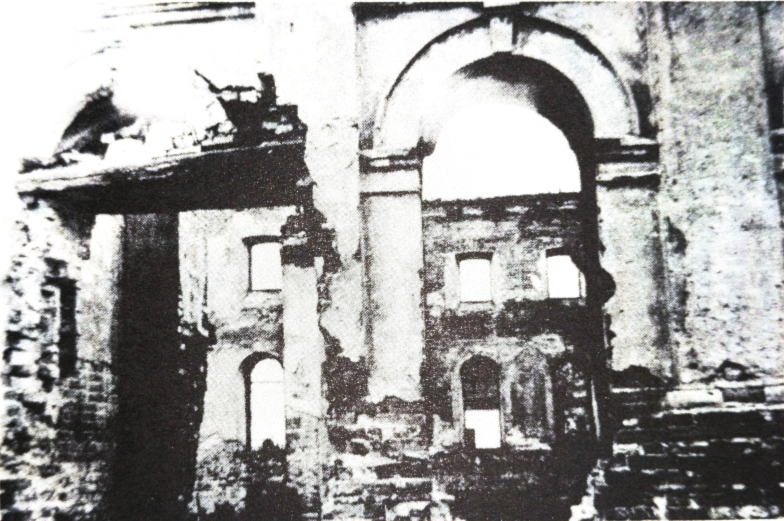
\includegraphics[width=7in]{Images/Saint_Mary_Church.png}}% Image to be included}
  \rotatebox{90}{% Rotate 90 CCW
    \begin{minipage}{\wd\stmary}
      \usebox{\stmary}
      \caption{Optina, the Church of St. Mary of Egypt --1978}
    \end{minipage}}
\end{figure}
\vspace*{\fill}\restoregeometry

\addcontentsline{toc}{chapter}{Glossary}
\chapter*{Glossary\markboth{Glossary}{}}

\begin{hangparas}{.25in}{1}
	\label{akathist}
	\gloss{akathist}{A series of hymns consisting of thirteen kontakia (short hymns), each followed by a refrain, and the first twelve followed also by an \textit{oikos} (pl. textit{oikoi}) (an intoned or chanted hymn).}
	
	\label{hegumen}
	\gloss{hegumen}{An abbot, a superior of a monastic establishment.}
	
	\label{hierodeacon}
	\gloss{hierodeacon}{A monk who has been ordained to the diaconate.}
	
	\label{hieromonk}
	\gloss{hieromonk}{A monk who has been ordained to the priesthood.}
	
	\label{hiero-schemamonk}
	\gloss{hiero-schemamonk}{A schemamonk (see below) who has been ordained to the priesthood.}
	
	\label{litya}
	\gloss{litya}{(Gk. \textit{liti}) Literally, ''Entreaty.'' A special service of supplication chanted during Great Vespers, usually in the narthex of the church.}
	
	\label{mantia}
	\gloss{mantia}{(Gk. \textit{mandias}) The outer garment of a monk, a wide garment, very long, and without sleeves, worn as a cape over his other monastic garments. This is given at the tonsure of a rassophor monk into the lesser schema, at which one pronounces vows and becomes a monk proper. Hence, to be tonsured into the mantia is to become a full-fledged monk.}
	
	\label{moleben}
	\gloss{moleben}{A special service of prayers of thanksgiving and petition offered on the occasion of some special occurrence in the life of an individual or of the nation. A \textit{moleben} may be requested at a time of special need or at a time of special thanksgiving. Somewhat equivalent to the \textit{Paraclesis}.}
	
	\label{nabedrennik}
	\gloss{nabedrennik}{A rectangular article of the priest's vestments, suspended by a shoulder strap, worn at the side hanging down from the waist. This article is bestowed by a bishop as an ecclesiastical dignity. It is not to be confused with the diamond shaped \textit{palitsa}, which may be given subsequently. This latter corresponds to the Greek \textit{epigonation}.}
	
	\label{pannikhida}
	\gloss{pannikhida}{A special service of prayers offered on behalf of the faithful who have reposed. At the service a dish of boiled wheat or rice with honey is set forth. A \textit{pannikhida} may be offered in conjunction with the Divine Liturgy or may form a separate service. This may be offered in church or at the grave of the reposed.}
	
	\label{paraman}
	\gloss{paraman}{The name derives from the Greek \textit{paramandias} meaning ``something besides, or added to the mantia.'' This is a square of material on which is depicted the Cross of Christ with the lance and reed and the inscription. ``I wear upon my body the wounds of my Lord.'' By means of cords or ribbons tied to each corner it is fastened around the shoulders and waist of the monk. This is given to monastics at the tonsure into the mantia.}
	
	\label{Philokalia}
	\gloss{Philokalia}{A compilation of exalted texts on prayer and the spiritual life which span from the fourth to the fifteenth centuries, compiled by SS. Macarios of Corinth and Nicodemos of the Holy Mountain, first printed in 1792. An abridged translation into Russian, the \textit{Dobrotolyubie}, by St. Paissy Velichkovsky, appeared in 1793. In the Elder Joseph's own days the edition of Theofan the Recluse appeared, considerably longer than the original, some 3,000 pages in all.}
	
	\label{prosphora}
	\gloss{prosphora}{The specially-prepared bread stamped with the Eucharistic Seal which is brought by the faithful to church to be used at the preparation of the Holy Eucharist. The faithful submit with the prosphora names of the living and the reposed to be commemorated at the preparation. The priest, having commemorated the names and having removed portions, placing them on the holy paten, returns the remainder of the prosphora to the one who submitted it. Prosphora so used may also be kept and distributed afterwards as a blessing from the Divine Liturgy.}
	
	\label{rassophor}
	\gloss{rassophor}{The name derives from the rassa, the robe with wide sleeves, and means ``wearer of the rassa.'' A rassophor monk has been tonsured into the monastic estate, but as yet has pronounced no vows.}
	
	\label{schema}
	\gloss{schema}{A piece of material decorated with many crosses and inscriptions, also called the \textit{analavon}, worn by monks tonsured into the highest state of monastics.}
	
	\label{schemamonk}
	\gloss{schemamonk}{The highest state of monastics, a monk tonsured into the great schema takes vows of complete renunciation of the world. In place of the \textit{paraman} he wears the \textit{analavon}, or schema, which is ornamented with many crosses and worn suspended from the shoulders.}
	
	\label{Typicon}
	\gloss{Typicon}{The book that contains the rule or order for the daily offices chanted in church. In the monastic context, it signifies also the Rule adhered to by a monastic community.}
\end{hangparas}

\bigpicgeometry
\vspace*{\fill}
\thispagestyle{empty}
\newsavebox{\map}
\begin{figure}[ht]
\center
  \savebox{\map}{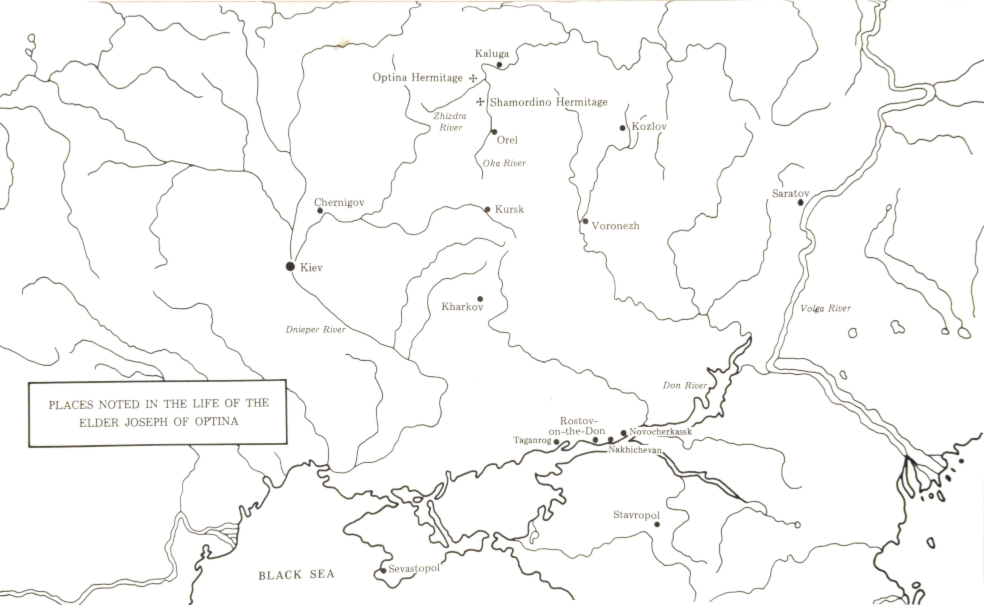
\includegraphics[width=8.5in]{Images/Optina_Map.png}}% Image to be included}
  \rotatebox{90}{% Rotate 90 CCW
    \begin{minipage}{\wd\map}
      \usebox{\map}
    \end{minipage}}
\end{figure}
\vspace*{\fill}\restoregeometry
\end{document}
